\documentclass[12pt]{caltech_thesis}
\usepackage[hyphens]{url}
\usepackage{graphicx}
\usepackage{hyperref}
\usepackage{minted}
\usepackage{listings}
\usepackage{pdflscape}
\usepackage{booktabs}
\usepackage{mathtools}
\usepackage{stackengine}
\usepackage{gensymb}

% Better Times fonts
\usepackage[utf8]{inputenc}
\usepackage{newtxtext,newtxmath}
\usepackage[T1]{fontenc}
\usepackage{microtype}
% Math fonts
\usepackage{amsmath}
\usepackage{amsfonts}
\usepackage{bm}
% Optimization defintions
\usepackage{optidef}
% Units
\usepackage[group-minimum-digits=4,per-mode=fraction]{siunitx}
% Crazy vector graphics
\usepackage{tikz}
\usepackage{pgfplots}
\usepackage[siunitx, american]{circuitikz}
% Various utils
\usepackage[version=4]{mhchem}
\usepackage[super]{nth}
\usepackage{algorithmic}
\usepackage{algorithm}
\usepackage{threeparttable}
\usepackage[subpreambles]{standalone}
\usepackage[hang,flushmargin]{footmisc}
\usepackage[caption=false]{subfig}

% Bib backend
\usepackage[
    bibstyle=ieee,
    citestyle=numeric,
    isbn=false,
    doi=false,
    sorting=none,
    url=false,
    defernumbers=true,
    bibencoding=utf8,
    backend=biber,
    style=ieee
]{biblatex}
\addbibresource{main.bib}
\addbibresource{mypubs.bib}
\addbibresource{grex.bib}

% SI setup
\sisetup{separate-uncertainty=true, detect-all=true, output-complex-root=\ensuremath{\mathrm{j}}}
\DeclareSIUnit{\belmilliwatt}{Bm}
\DeclareSIUnit{\dBm}{\deci\belmilliwatt}
\DeclareSIUnit{\ounce}{oz}

% Tikz/pgf setup
\pgfplotsset{compat=1.18}
\usepgfplotslibrary{units}
\usepgfplotslibrary{fillbetween}
\usepgfplotslibrary{smithchart}
\usepgfplotslibrary{colormaps}
\pgfplotsset{table/search path={figures/data}}
\usetikzlibrary{positioning, shapes, arrows, arrows.meta, graphs, shapes.geometric, math}
\tikzset{>=latex} % Better arrow tips
\tikzset{
    value/.style = {rectangle, draw, fill=black!5, thick, minimum width=0.5cm,
                        minimum height = 0.5cm,align=center},
    computation/.style = {circle, draw, thick,align=center}
}

\usemintedstyle{xcode}
\newlength\longest

% Configure hyperref
\hypersetup{
  hidelinks,
  colorlinks=true,
  allcolors=black,
  pdfstartview=Fit,
  breaklinks=true
}

% My commands
\newcommand{\R}{\mathbb{R}}
\newcommand{\C}{\mathbb{C}}
\newcommand{\nuvec}{\bm{\nu}}
\newcommand{\xvec}{\bm{X}}
\newcommand{\sopt}{S_{\text{opt}}}
\newcommand{\GS}{\Gamma_{\text{S}}}
\newcommand{\GSp}{\Gamma_{\text{S}}^\prime}
\newcommand{\GL}{\Gamma_{\text{L}}}
\newcommand{\GLp}{\Gamma_{\text{L}}^\prime}
\newcommand{\GIn}{\Gamma_{\text{In}}}
\newcommand{\GOut}{\Gamma_{\text{Out}}}
\newcommand{\GOpt}{\Gamma_{\text{Opt}}}
\newcommand{\GA}{\Gamma_{\text{A}}}
\newcommand{\GB}{\Gamma_{\text{B}}}
\newcommand{\FMin}{F_{\text{Min}}}
\newcommand{\LN}{L\ce{N2}}

\newcommand{\fixme}[1]{\textcolor{red}{#1}}
\newcommand{\urlfootnote}[1]{\footnote{\raggedright\url{#1}}}

% Results as they get updated from more experiments
\newcommand{\newnoise}{\qty{11.53 \pm 0.42}{\K} }
\newcommand{\oldnoise}{\qty{12.48 \pm 0.42}{\K} }
\newcommand{\improvement}{\qty{0.95 \pm 0.59}{\K} }

% Better looking Re
\renewcommand{\Re}{\operatorname{Re}}

\renewcommand{\chapterautorefname}{Chapter}

\begin{document}

\title{Low Noise at Low Cost for \\ Large Radio Astronomy Arrays}
\author{Kiran Arik Shila}

\degreeaward{Doctor of Philosophy}         
\university{California Institute of Technology}  
\address{Pasadena, California}                   
\unilogo{figures/caltech.png}       
\copyyear{2025}
\defenddate{May 15, 2025}

\orcid{0000-0003-4652-7038}

\rightsstatement{Some rights reserved. This thesis is distributed under a Creative Commons Attribution-NonCommercial-ShareAlike License}

\maketitle[logo]

\clearpage
\null\vfill
\settowidth\longest{\large\itshape I come with empty hands and the desire to unbuild walls;}
\begin{center}
    \parbox{\longest}{%
  \raggedright{\large\itshape%
        I come with empty hands and the desire to unbuild walls\par\bigskip
  }   
  \raggedleft\tiny\MakeUppercase{Ursula K. Le Guin \\  The Dispossessed}\par%
}
\end{center}
\vfill\vfill
\clearpage

\begin{acknowledgements} 	 
    In the winter of 2018, I found myself at a crossroads in my career.
    I was finishing my Bachelor’s degree, had completed several internships and contracting jobs, and had done a bit of research at school.
    However, I was unsure about my next steps—whether to pursue something more academic, whether to focus on hardware or software, or even what I truly wanted to work on.
    Around that time, I was shown a posting for a summer job at Caltech, working with Sandy Weinreb on radio astronomy.
    I knew almost nothing about the field, but I seemed to have the “hands-on” radio experience Sandy was looking for, so I emailed him.
    Less than five minutes later—close to midnight in California—I received a reply asking if I could FaceTime him.
    We ended up talking for over two hours.
    That summer, I worked with Sandy and the team on hardware that would become part of the DSA-10 radio telescope, and I had more fun than I ever could have imagined.
    I would like to first and foremost thank Sandy for introducing me to this field and for providing invaluable mentorship over these years, forever altering the trajectory of my career.

    A few years later, after completing my Master’s degree, I was accepted to return to Caltech to pursue a PhD.
    Unfortunately, this was in the fall of 2020, at the height of the COVID-19 pandemic.
    As a result, I had to complete my first year of studies online, remotely from Florida—one of the most challenging educational experiences of my life.
    However, many of us quickly found a sense of community online with others around the world who were going through the same thing.
    Through this, I connected with the people who have since become some of my closest friends.
    Thank you to David, Elijah, Emma, Hannah, Ian, Isaac, Kyle, Nick, Quinn, Rhiannon, Sarah, Saren, Sasha, Steven, Talya, and Yoonsoo for including me in the world’s smartest clown car.

    Upon returning to Caltech, I was introduced to Professors Gregg Hallinan, Vikram Ravi, and Shri Kulkarni from the Astronomy department, all of whom provided invaluable guidance and support.
    I would like to thank Gregg, my advisor, who kept me focused on making an impact on our project's scientific goals.
    He also encouraged (and funded!) my travel to conferences around the world, where I met many collaborators who continue to inspire me.
    Vikram was instrumental in helping me bridge the gap between my engineering background and the world of astronomy.
    Shri proposed and funded my first project—the Galactic Radio Explorer (GReX)—and appointed me as the project engineer, for which I am deeply grateful.

    I would also like to especially acknowledge Steve Padin.
    One day in early 2022, I received a knock on my office door, and Steve introduced himself with the words, "I heard you need help."
    Since then, Steve has spent countless hours in the lab with me—checking my work, keeping me on track, and working through problems alongside me.
    He has been a key advisor, particularly on all aspects of engineering, always offering his time and support whenever I needed it.
    I truly do not know if I would have been able to complete this degree without him, and for that, I am sincerely grateful.
    
    Thank you to Liam Connor, who worked as project scientist for GReX.
    All the hours working on code and in the car driving back and forth to OVRO chatting about anything and everything is time I wouldn't trade for anything.

    I'd like to thank Schmidt Sciences for funding DSA-2000 and by extension my degree.

    Thank you to James, Mark, Francois, Katie, Vinand, Jonas, Dave, Charlie, and everyone else at OVRO and the DSA-2000 team.

    Thank you to David Hodge and Courtney Keeler for all the help in the lab.

    Thank you to Jack, Jonathan, Mitch, Morag, Dan, Kathryn, and the rest of the CASPER collaboration.

    Thank you to Glenn Price, Barb Caitlin, Scott Babcock, and the rest of the folks from Caltech's performing and visual arts for the incredible time with the Wind and Symphonic Orchestra, Percussion Ensemble, and Jazz big band and improv group.
    You all gave me a much-needed artistic outlet and a way to engage with LA's musical community.

    Thank you to my committee, Professors Gregg Hallinan, Vikram Ravi, Steve Padin, Katie Bouman, Ali Hajimiri, and Alireza Marandi for helping me through candidacy and the final steps of my degree.

    Finally, I'd like to thank my wonderful partner Ivy and our cat, Rocket, for moving across the country to support me in this crazy degree.
    Lastly, to my mother, who gave me love, support, and strength through this wild ride.
    I love you all.
\end{acknowledgements}

\begin{abstract}
   The 2020s is the decade of survey instruments in astronomy.
   Radio astronomy is no exception, with Caltech's proposed DSA-2000 being the most powerful radio interferometer in the world, costing much less than competing instruments.
   Key to this achievement are two core breakthroughs, a completely ambient-temperature receiver and a ``radio camera'' backend that images the sky in real time.
   DSA-2000 will have record-breaking survey speed and sensitivity, enabled by these two key breakthroughs, giving astronomers all over the world open access to exquisite all-sky maps to enable the discovery of billions of new radio sources, precise timing of pulsars, and localization of fast radio bursts.
   The array will produce enough data to keep astronomers busy for a century.

   In this thesis, we discuss the development of one of the key breakthroughs, the ambient-temperature receiver.
   Specifically, we focus on the design, testing, and implementation of the wideband, ambient-temperature low noise amplifier.
   We cover the design from analytic first principles through precision measurement of its performance.
   We follow this with a discussion of the design and implementation of the analog signal path, including a high performance, analog over fiber backhaul link.
   Finally, we discuss the Galactic Radio Explorer (GReX) instrument, designed as a global experiment probing the brightest radio transients in the local universe.
\end{abstract}

\begin{publishedcontent}[iknowwhattodo]
\nocite{shilaRapidDesignLNASubmitted}
\nocite{shilaGReXInstrumentOverviewSubmitted}
\end{publishedcontent}

\tableofcontents
\listoffigures
\listoftables

\mainmatter

\chapter{Introduction} \label{ch:intro}
\begin{refsection}
% This chapter is pretty flowery, but so am I *shrug*
\section{The Decade for Surveys}

One would be hard-pressed to find a better time to be working in astronomy than at this moment.
Amazing new instruments are coming online that are pushing the boundaries of what can be observed, giving astronomers a deluge of data to explore and new secrets of the universe to unlock.
For engineers, every new instrument starts as a question, “What is possible?”
Every year the answer changes as technology progresses, giving astronomers more compute power, more sensitivity, and lower costs.

This decade is especially exciting with the deployment of a slew of powerful new instruments.
Specifically, we are seeing an emphasis on survey instruments, mapping out the sky across the entire EM spectrum.
These types of experiments are not proposal-based where one would request to look at some interesting object, instead relying on the community at large to explore the data, searching for patterns, outliers, and really anything interesting.
This is well-motivated, as most major discoveries in astronomy were serendipitous.
Having such a large volume of data across parameter space enables discovery of the unexpected, assuming we are prepared~\cite{norrisDiscoveringUnexpectedAstronomical2017}.
Additionally, surveys democratize science by enabling everyone to explore the rich datasets, instead of allowing only a select few whose proposals were accepted to have access to high-quality data.
All this is to say that surveys are a key tool in modern astronomy and are consistently ranked among the highest priority in science funding~\cite{nationalacademiesofsciencesPathwaysDiscoveryAstronomy2023}.

In the optical, the Vera Rubin Observatory in Chile will soon conduct a massive all-sky survey~\cite{biancoOptimizationObservingCadence2021}, with a projected first light in July 2025.
The recently launched SPHEREx satellite~\cite{crillSPHERExNASAsNearinfrared2020} will survey the near infrared and will be starting its survey soon.
In the radio, the VLA Sky Survey (VLASS)~\cite{lacyKarlJanskyVery2020} is ongoing, imaging the whole sky visible to the VLA in New Mexico.
This experiment builds off the success of previous VLA-based surveys\footnote{Which are some of the most scientifically successful experiments that the VLA has performed}, further improving sensitivity and resolution.
While continuing to be successful, the speed at which VLASS images the sky is comparatively very slow.
Rubin images \qty{10}{deg^2} every \qty{15}{\s} or \qty{2400}{deg^2/hr} (during the nighttime).
SPHEREx will survey the entire sky once every six months, or a speed of \qty{5}{deg^2/hr}.
Finally, VLASS operates at about \qty{0.01}{deg^2/hr}, while splitting time between the survey and other planned observations.
Even though VLASS (and previous radio surveys) are very successful, they are being executed on instruments poorly optimized for surveys.

This is where the Deep Synoptic Array 2000 (DSA-2000)~\cite{hallinanDSA2000RadioSurvey2019} comes in.
Rather than using existing radio telescopes to survey the sky, we propose a bespoke survey instrument to match the scale and cadence of surveys from other wavelengths.
This will result in a massive legacy dataset that will be transformative in radio astronomy and produce enough data to keep astronomers busy for decades to come.

\section{Designing A Survey Instrument}

In the design of a survey instrument, the key metric is the speed at which we can create images of the sky.
The faster we can make high-sensitivity maps, the faster we can get these maps in the hands of astronomers to do science.
We can quantify this measure via survey speed, defined as the time required to map one patch of sky down to some fixed noise level
\begin{equation}
        \text{SS}~(\text{deg}^2/\text{hr}) \approx 1.217\eta_a\Delta_\nu\left[\frac{\lambda S_\nu N D}{T_\text{Sys}}\right]^2
\end{equation}
This equation for the survey speed of reflector-based radio telescope arrays (derived in \autoref{sec:survey_speed}), depends on the number of antennas $N$, the system noise temperature $T_\text{Sys}$, the diameter of the dishes $D$, the aperture efficiency of the dishes $\eta_a$, the observation wavelength $\lambda$, the integration bandwidth $\Delta_\nu$, and the desired $1\sigma$ flux density $S_\nu$ in Jy.
In essence, this metric combines the sensitivity of the instrument with how much of the sky it can see.
One could also just ask about that sensitivity, given by
\begin{equation}
    S_\nu~(\mu\text{Jy @ 1 hr}) \approx 1852\frac{T_\text{Sys}}{\eta_aD^2N\sqrt{\Delta_{\nu\text{(GHz)}}}}
\end{equation}
which gives the RMS noise in $\mu$Jy in one hour of integration.
The ideal instrument would have a minimal noise and a large collecting area, which corresponds to a high survey speed.

\begin{figure}[ht!]
    \centering
    \includestandalone[mode=buildnew]{figures/dsa2000_compare}
    \caption{Comparison of radio telescopes at \qty{1.4}{\GHz} in survey speed and sensitivity}
    \label{fig:dsa2000_compare}
\end{figure}

Using these metrics, we can compare the planned DSA-2000 performance against other planned and deployed instruments.
DSA-2000 will be composed of 2000, \qty{5}{\m} dishes operating at an aperture efficiency of about \num{0.7}, observing from \SIrange{0.7}{2}{\GHz} with a system noise temperature of about \qty{25}{\K}.
For this comparison, we will look at DSA-110~\cite{raviDSA110OverviewFirst2023}, ASKAP~\cite{hotanAustralianSquareKilometre2021}, MeerKAT~\cite{jonasMeerKATRadioTelescope2018a}, CHORD~\cite{vanderlindeCanadianHydrogenObservatory2019}, 
VLA~\cite{VLAObservationalStatus}, and ngVLA~\cite{NgVLAPerformanceEstimates}, shown in \autoref{fig:dsa2000_compare}.
With these results, we can see that the DSA-2000 outperforms all instruments in this band in survey speed, with only ngVLA having higher sensitivity.
This is not too surprising as the ngVLA is a multi-billion dollar project with large, cryogenically cooled receivers.
If we quantify the science output of these instruments as proportional to their survey speed\footnote{A somewhat dubious claim, but good enough for this exercise}, and then try to predict science per dollar, we see a very different story.

The construction costs for a radio telescope array can be broken down into two major chunks: the processing hardware and the antennas themselves.
For an $N$-antenna array, the cost of the compute scales with $N^2$.
We will ignore operation cost and everything else just so we can get a grasp on the design-space.
To keep costs low, it would seem that we would want to keep $N$ low, but our survey speed \textit{increases} by $N^2$, so these are certainly at odds.
Currently, compute is relatively inexpensive for the kind of processing we need to do, at least compared to the cost of the antenna hardware itself.
Our current estimates for DSA-2000 put the cost of the compute (again ignoring power, installation, operations, etc.) at around \$20M for 2000 antennas.
The antennas cost about \$30k each, for a total of \$60M before trenching, installation, etc.
Compare this to  ngVLA's much larger, cryogenically cooled antennas, which cost about \$7M each.

% \begin{figure}[ht!]
%     \centering
%     \includestandalone[mode=buildnew]{figures/ss_per_dollar}
%     \caption[Survey speed for fixed budget]{Survey speed for a fixed budget of \$100M}
%     \label{fig:ss_per_dollar}
% \end{figure}

% Designing a sensitive antenna can be expensive, so an important question is how to spend your money.
% If you designed an expensive, cryogenic receiver like the ngVLA, you will certainly win in sensitivity.
% However, at some point, one could imagine that many cheap antennas might beat the expensive solution at scale.
% Again, assuming a fixed compute cost scaling, the price per antenna (and the sensitivity of each antenna) is really what matters.
% We can better visualize this by looking at the sensitivity of a few instruments, given a fixed budget of \$100M, shown in \autoref{fig:ss_per_dollar}.

% In \autoref{fig:ss_per_dollar}, we include a point for DSA-10~\cite{koczDSA10PrototypeArray2019}, a last-generation pathfinder instrument.
% DSA-10 had a system temperature of around \qty{60}{\K}, but was relatively inexpensive to build.
% DSA-110 was a progression on this design, with massive improvements in the LNA~\cite{weinrebLowNoiseAmplifier2021} reducing the system noise to \qty{25}{\K}.
% Finally, we see DSA-2000 at the top of the plot.
% DSA-2000's antennas are pricier, which reduces the number that one could build with a fixed budget, but the tradeoff still improved survey speed per dollar.
% For comparison, we include 15 ngVLA antennas, which is about what you could build with this fixed budget.

Matching the ngVLA, we could add cryogenics to cool the DSA-2000 receiver to \qty{20}{\K}, which would cost about \$100k per antenna~\cite{daddarioAdvancedCryocoolersNext2017}.
Simulations predict this will reduce our system noise temperature by \qty{7}{\K} to \qty{18}{\K}, as cooling only impacts the feed and LNA and there are still other sources of noise (the sky, spillover noise, etc. See \autoref{fig:tsys_contributions}).
If each antenna costs around \$30k, we quadruple the cost of each antenna, while not even doubling the survey speed.% (\qty{32}{deg^2/hr} to \qty{63}{deg^2/hr}).

All of this leads to the conclusion that if you can build a high-performance, cheap antenna, build lots of them!
And the key to an inexpensive antenna is not using cryogenics.
As survey speed scales with $T_\text{Sys}^{-2}$, any reduction in system noise will dramatically increase the science per dollar of the instrument.
The strong impact of reducing noise then motivates the work in this thesis, where reducing the system noise by even \qty{1}{\K} would save about \$1M in cost to maintain survey speed.
Of all the contributions to $T_\text{Sys}$, currently the LNA is the largest (as shown in \autoref{fig:tsys_contributions}) which suggests where to spend effort to maximize the impact on the science.

\begin{figure}[ht!]
    \centering
    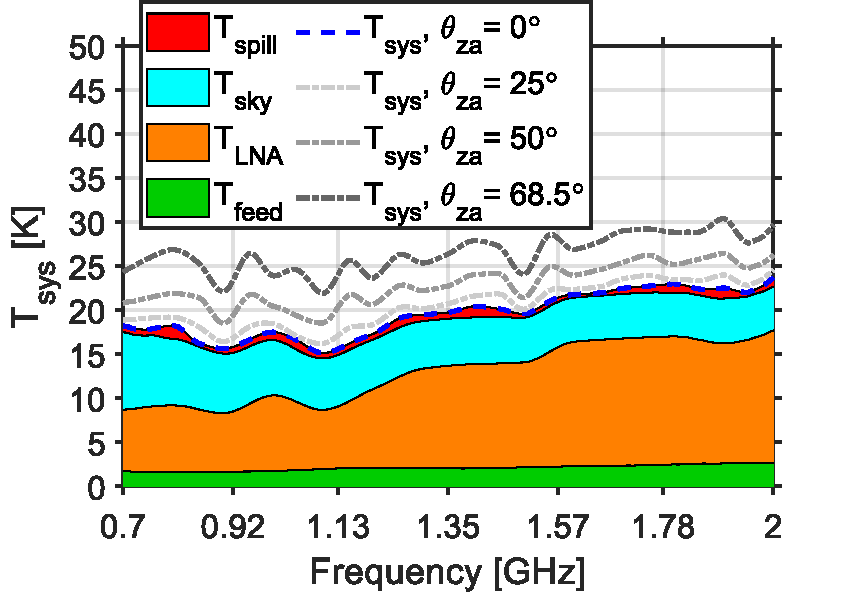
\includegraphics[width=0.8\textwidth]{figures/DSA2000_Tsys.pdf}
    \caption[DSA-2000 system noise temperature contributions]{DSA-2000 system noise temperature contributions. Reproduced from~\cite{flygareWidebandLowLossFeed2024} with permission from J. Flygare.}
    \label{fig:tsys_contributions}
\end{figure}

If it is so obvious to build a large $N$ telescope, a reasonable question would be, “why haven't people done this before?”
To answer this, we need to discuss a bit more about radio telescope interferometers.

Radio telescopes were historically built using a single, large aperture.
A large collecting area increases sensitivity and resolution, but the cost of building a large reflector with diameter $D$ is $\propto D^{2.5-2.7}$~\cite{belleScalingRelationshipTelescope2004}.
Additionally, there are practical upper limits on the size of a reflector one could build, with the largest single-dish antenna being the FAST telescope in China at \qty{500}{\m} in diameter, with a \qty{300}{\m} effective aperture.
At a typical observation frequency of \qty{1.4}{\GHz}, the diffraction-limited resolution of FAST is \qty{3}{arcmin}.
Compare this with a modest optical observatory such as Keck, with a \qty{10}{\m} mirror, where they achieve an angular resolution of better than \qty{0.05}{arcsec}.

To overcome this resolution shortcoming, the concept of radio interferometry was developed by Ruby Payne-Scott and Joseph Pawsey in the 1940s.
They used the interference pattern produced by combining radio signals reflecting off the ocean with a receiver on top of a cliff to pinpoint emission from sunspots.
This essentially provided them with the angular resolution of a telescope the size of the distance from their antenna to the image of their antenna in the ocean.
This concept was further developed by Martin Ryle and Antony Hewish in the 50s, where they used Earth's rotation to synthesize a massive equivalent aperture.
This technique is so powerful, it was part of Ryle and Hewish's Nobel Prize in Physics in 1974\footnote{Which, notably, did not include Jocelyn Bell who actually discovered the first pulsar to which the Prize was attributed}.
Modern aperture synthesis uses a combination of spatially distributed antennas and Earth rotation to synthesize a single massive telescope.
Very long baseline interferometry (VLBI) has receivers all over the world to synthesize an Earth-sized telescope, used to create the first images of a black hole~\cite{eventhorizontelescopecollaborationFirstM87Event2019}.

The radio interferometer imaging procedure starts with the coherent combination of the time-averaged product of signals from pairs of antennas.
As the signal from the sky is essentially incoherent noise, this result is a statistical correlation product between antennas.
The surprising result is that there exists a relationship between the collection of all these correlation products (known as visibilities) and the image of the sky.
This relationship is known as the van Cittert-Zernike theorem\footnote{Using a small angle approximation, which results in the Fourier relationship} and states
\begin{equation}
    V(\mathbf{r}_1,\mathbf{r}_2) \approx \iint_{-\infty}^{\infty}I(l,m)e^{-2\pi j(ul+vm)}dldm = \mathcal{F}\{I(l,m)\}
\end{equation}
where $V(\mathbf{r}_1,\mathbf{r}_2)$ is the visibility or mutual spatial coherence function given by the time average product of the received signal (electric field) from the pair of antennas at two points in space ($\mathbf{r}_1$ and $\mathbf{r}_2$)
\begin{equation}
    V(\mathbf{r}_1,\mathbf{r}_2) = \langle E(\mathbf{r}_1)E(\mathbf{r}_2)^*\rangle
\end{equation}
and $u$ and $v$ are the spatial differences between the two points\footnote{Ignoring changes in height $z$, which is something you might want to consider~\cite{cornwellProjectionNewAlgorithm}}
\begin{equation}
    \mathbf{r}_1 - \mathbf{r}_2 = \mathbf{u} = (x_1-x_2, y_1 - y_2) = (u,v)
\end{equation}
and $I(l,m)$ is the intensity distribution (image) of the sky in a direction-cosine reference frame.
All of this is to say that the inverse Fourier transform of the visibilities gives us the image of the sky!
%
\begin{figure}[ht!]
    \centering
    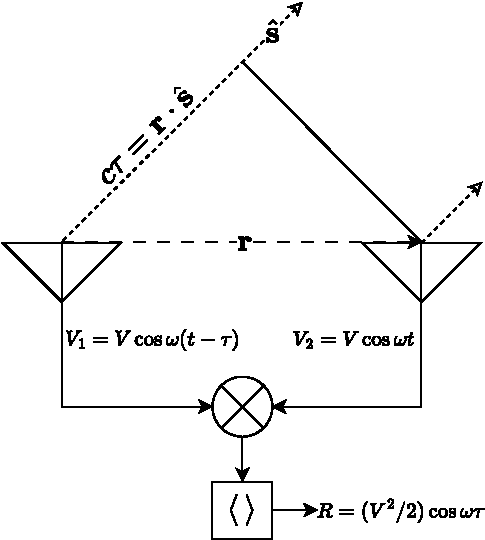
\includegraphics[width=0.5\textwidth]{figures/radio_interferometer.pdf}
    \caption{Diagram of a radio interferometer}
    \label{fig:interferometer_diagram}
\end{figure}

A problem then arises from the fact that we have not continuously sampled all the points in $u$ and $v$ as we have a discrete number of antennas and therefore a finite number of visibilities.
Not only that, but there is a maximum distance that we can separate antennas.
Combining these two shortcomings, we essentially image the sky through a diffraction-limited, shattered mirror.
This imaging procedure is shown in \autoref{fig:radio_imaging} as Fourier pairs, where a sparse sampling of the Fourier-domain of the true image of the sky results in the measured, dirty image.
The dirty image itself is not usable for science, so we must attempt to recover the true image algorithmically.
However, due to the sparse sampling of the $uv$ plane, this is an ill-posed inverse problem and does not have a simple solution.
Various optimization-based strategies are used for this, perhaps the most popular being an iterative blind deconvolution algorithm called CLEAN~\cite{hogbomApertureSynthesisNonRegular1974}.

\begin{figure}[ht!]%
    \centering
    \setlength{\tabcolsep}{1pt} % spacing between columns
    %\renewcommand{\arraystretch}{1} % spacing between rows
    \begin{tabular}{ccccc}
        \captionsetup{position=top}
        \subfloat[True Image]{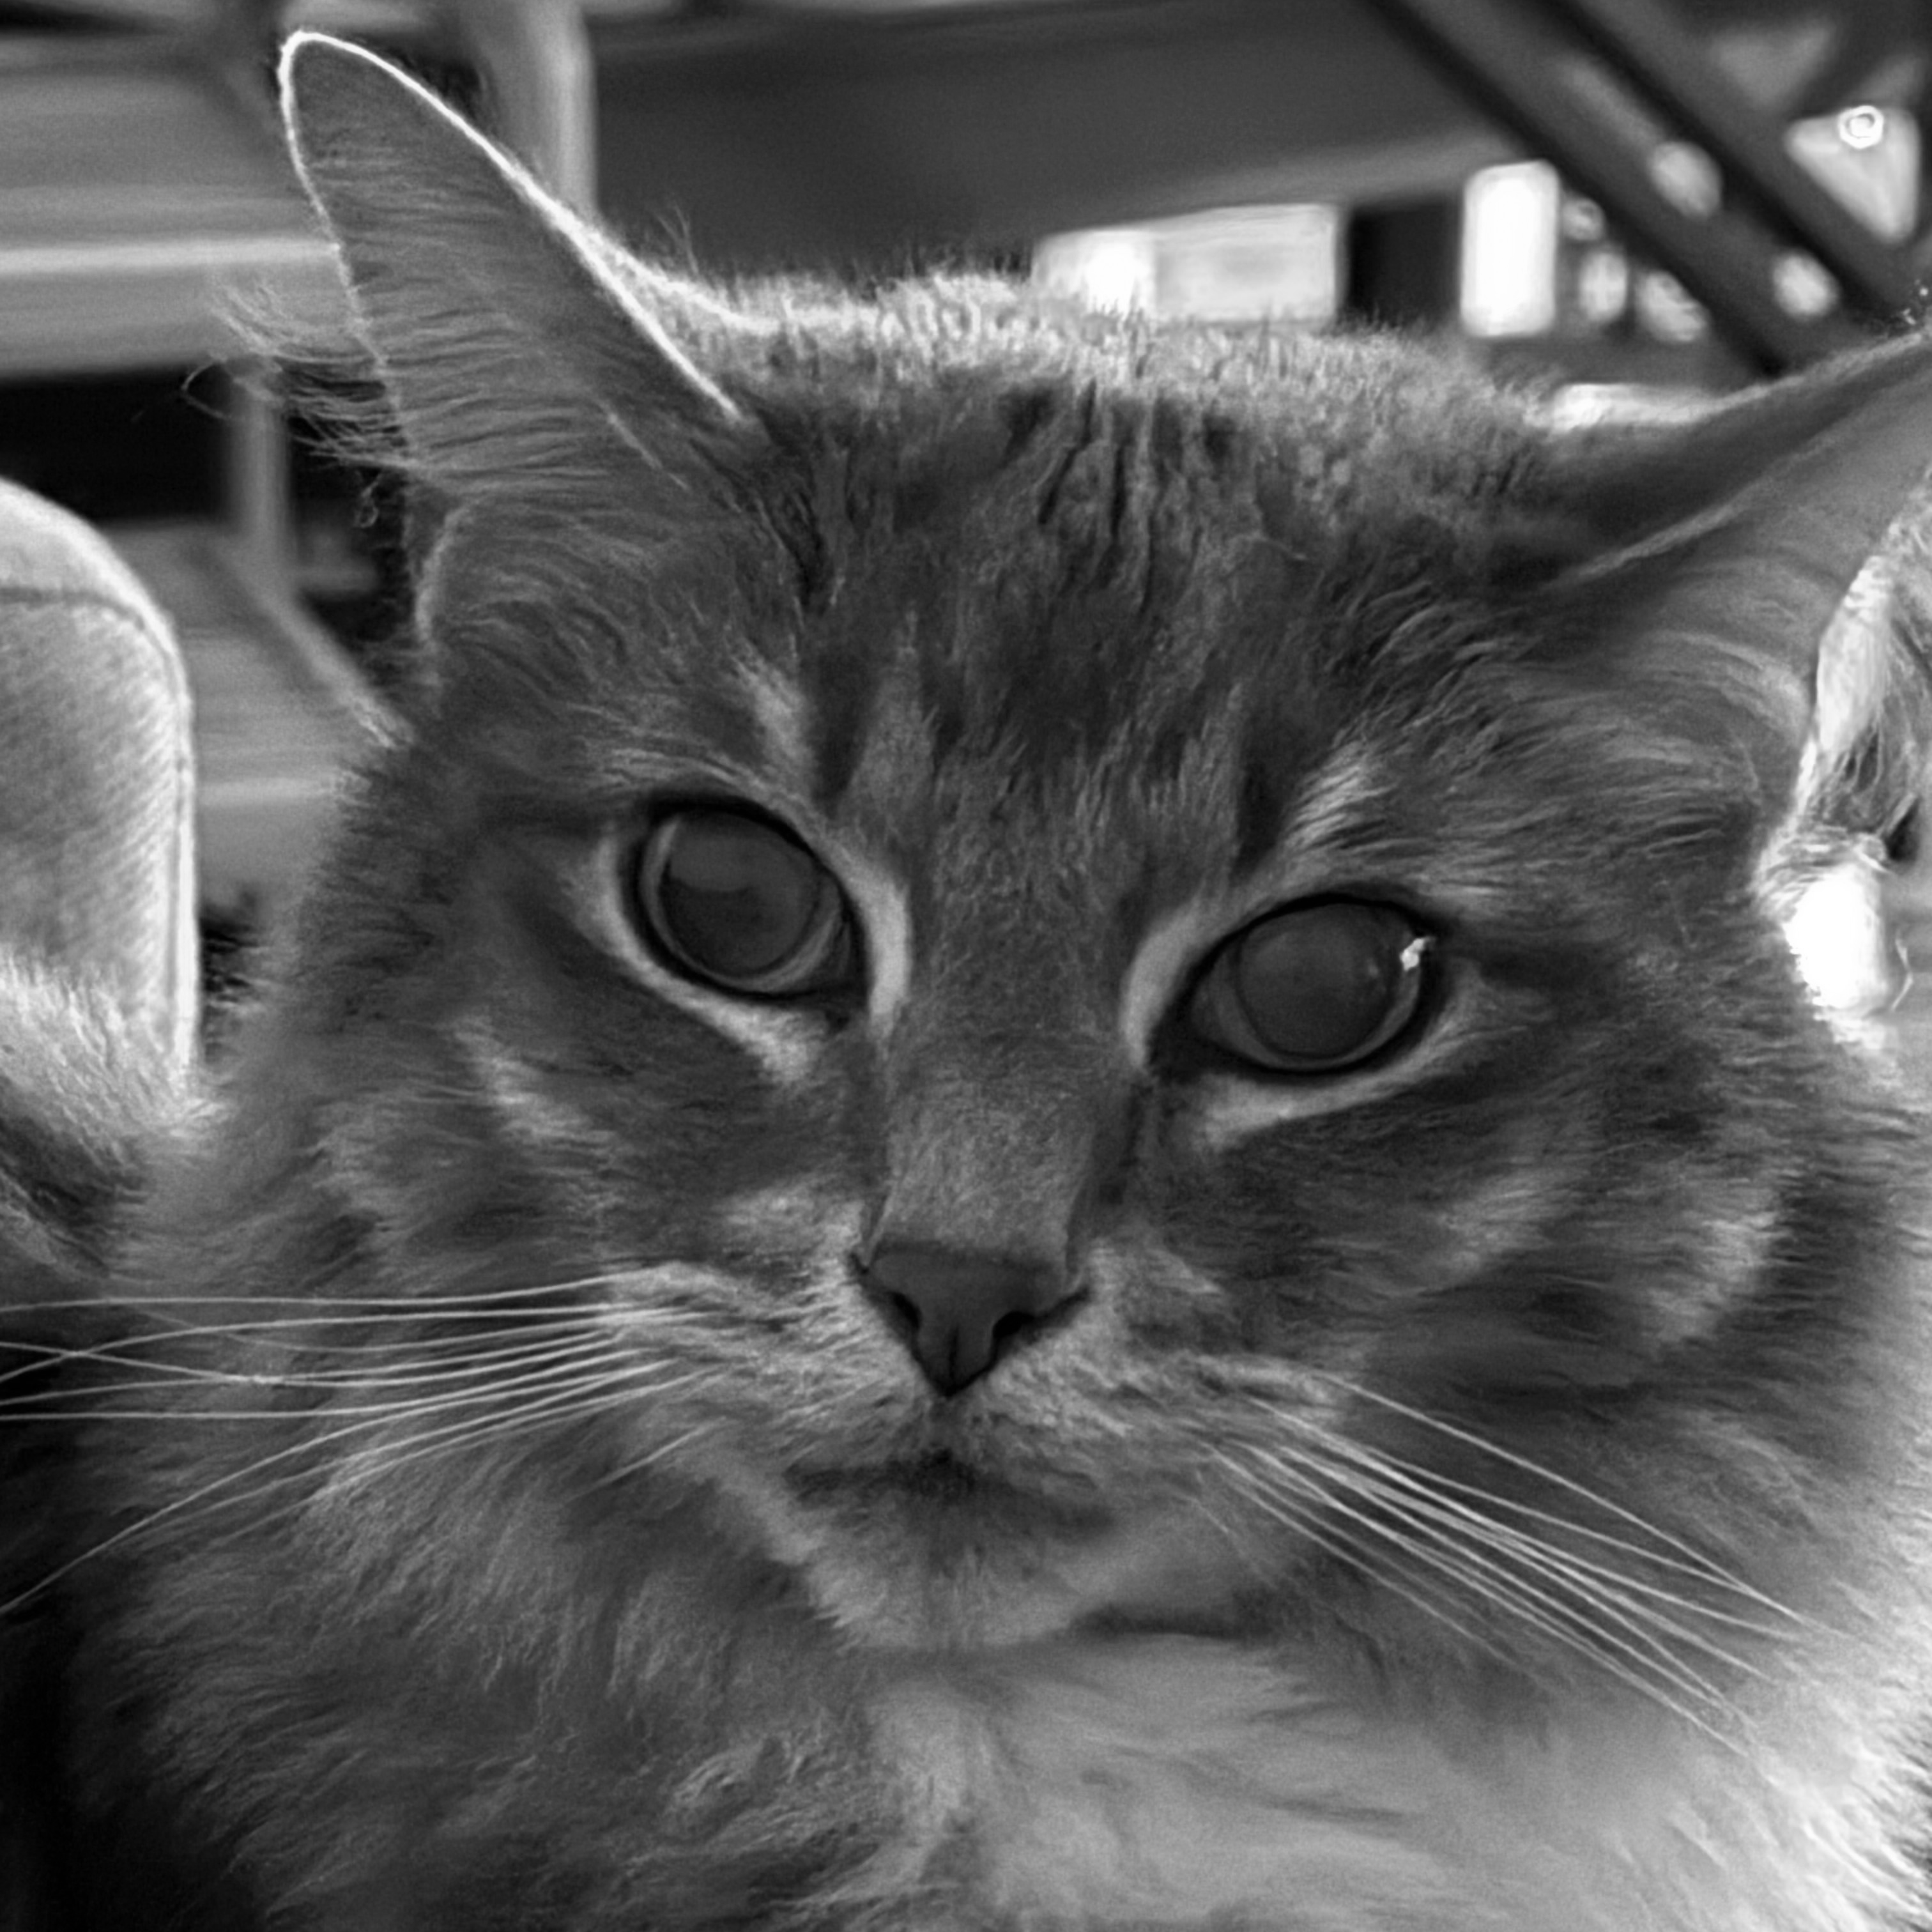
\includegraphics[height=4cm]{figures/rocket.png}} &
        \raisebox{-2.2cm}{$\scalebox{1.5}{$\circledast$}$} &
        \captionsetup{position=top}
        \subfloat[Point-Spread Function]{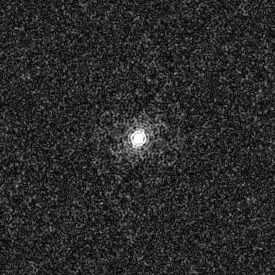
\includegraphics[height=4cm]{figures/psf.png}} &
        \raisebox{-2.2cm}{$\scalebox{1.5}{$=$}$} &
        \captionsetup{position=top}
        \subfloat[Dirty Image]{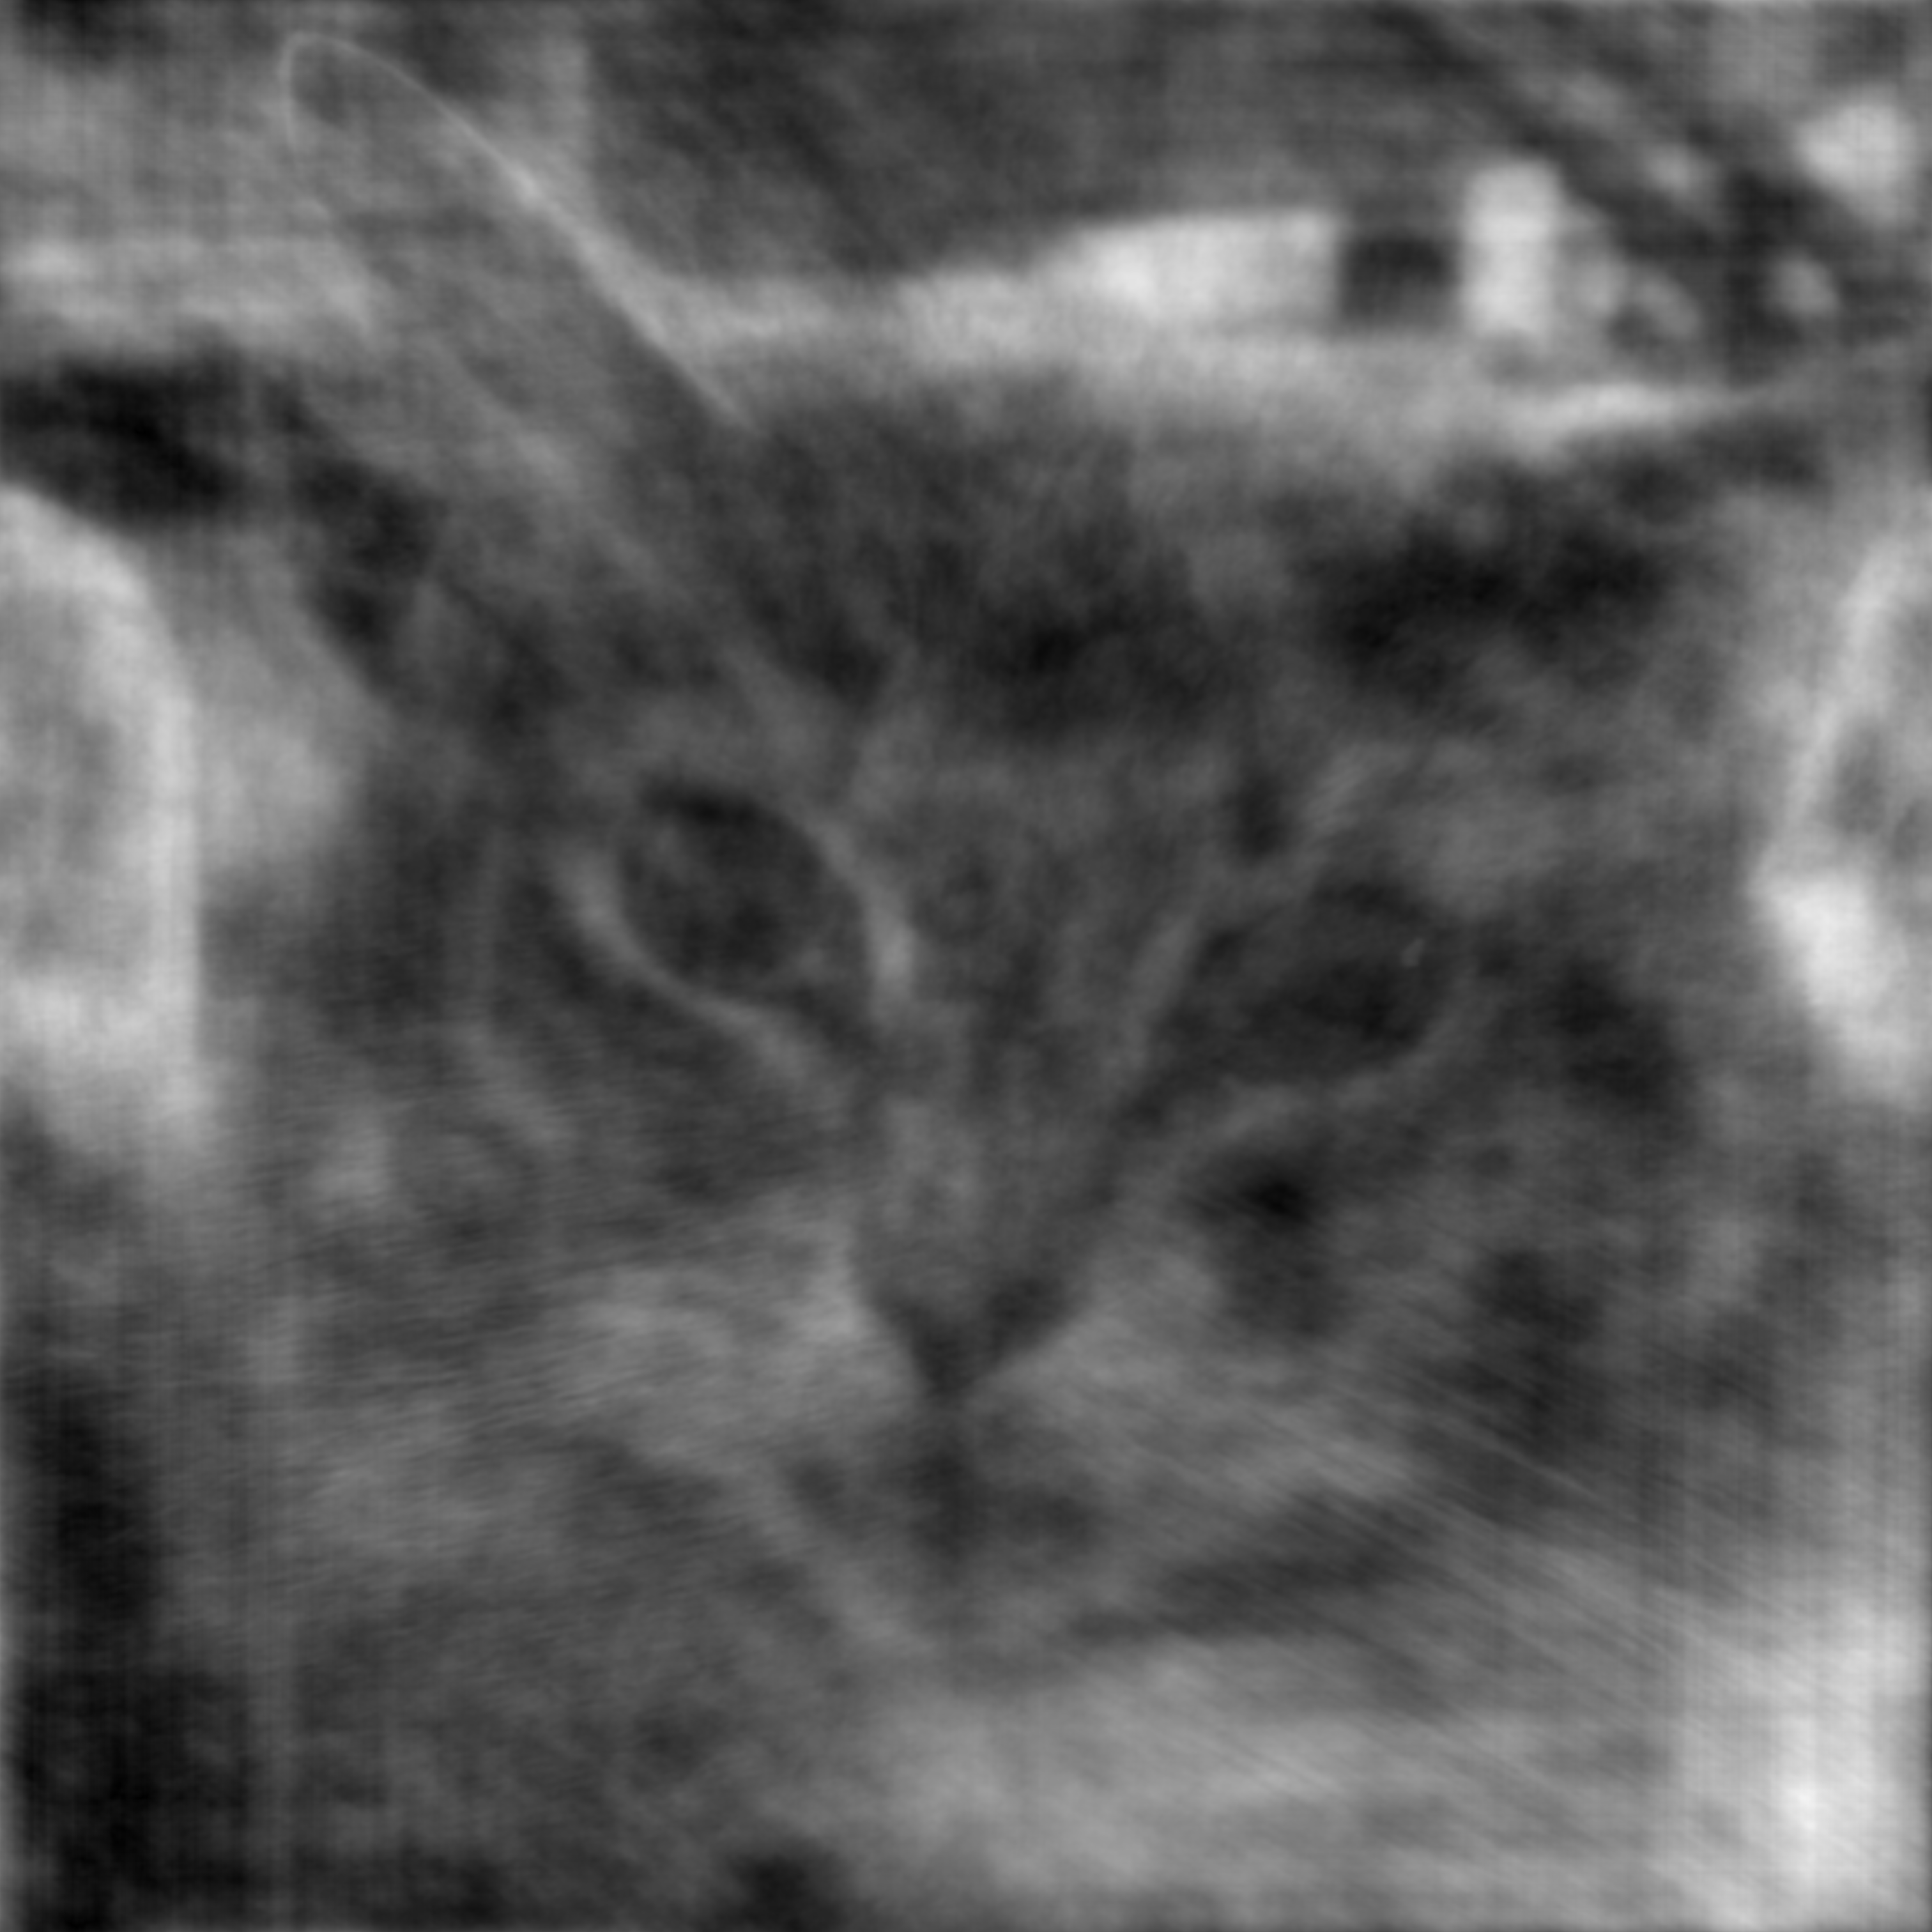
\includegraphics[height=4cm]{figures/dirty_image.png}} \\
        
        \multicolumn{5}{c}{\scalebox{1.5}{$\uparrow\mathcal{F}\downarrow$}} \\

        \subfloat[True Visibilities]{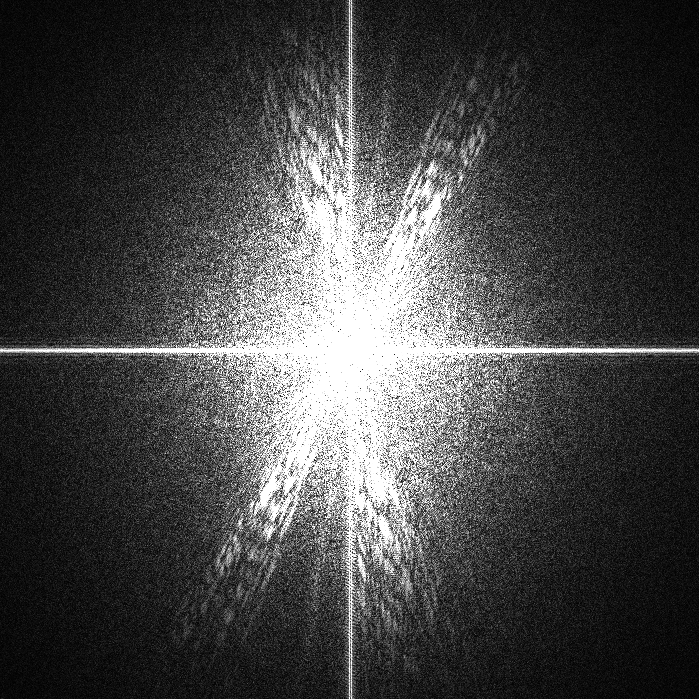
\includegraphics[height=4cm]{figures/true_response.png}} &
        \raisebox{1.84cm}{$\scalebox{1.5}{$\times$}$} &
        \subfloat[Sampling Function]{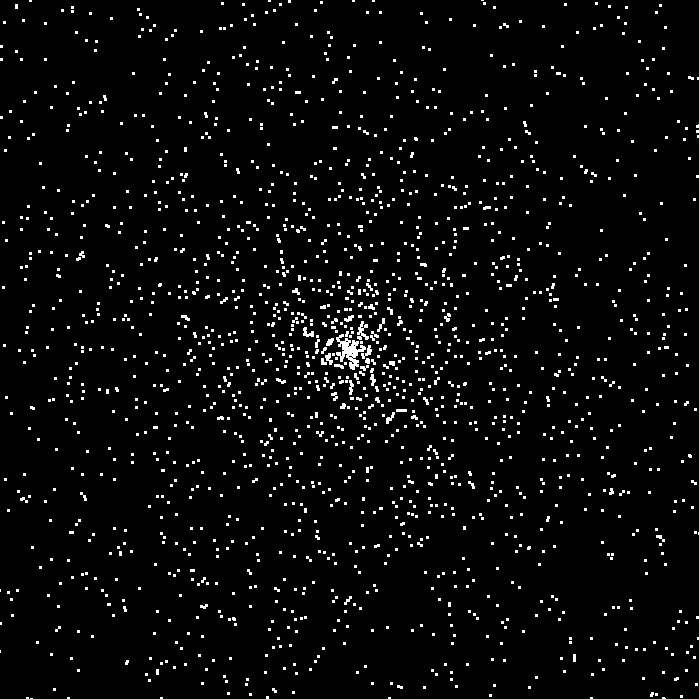
\includegraphics[height=4cm]{figures/sample_fun.png}} &
        \raisebox{1.84cm}{$\scalebox{1.5}{$=$}$} &
        \subfloat[Sampled Visibilities]{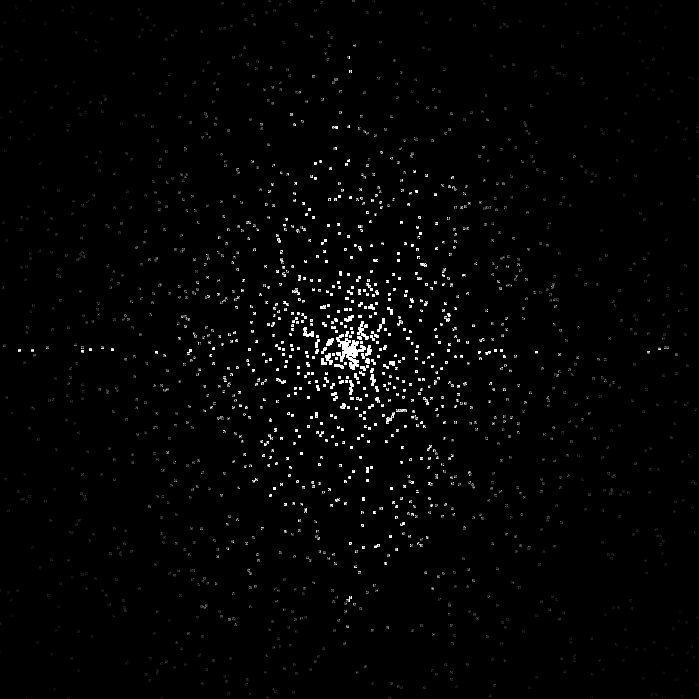
\includegraphics[height=4cm]{figures/sampled_response.png}} \\
    \end{tabular}
    \caption{Radio interferometer Fourier pairs}
    \label{fig:radio_imaging}%
\end{figure}

As we increase the number of antennas and the area they cover, we fill out the $uv$ plane more and more, resulting in a better image.
In the same manner as survey speed, this encourages us to build a telescope with bigger $N$.
However, the tradition in radio astronomy is to distribute the raw visibilities as the data product.
In sparse arrays like the Very Large Array, or the Event Horizon Telescope, the scientist performing the analysis might want full control over how the image is formed from the sparse data, making their own assumptions on how to interpret them.
For DSA-2000, let us assume we observe \num{16000} frequency channels every \num{10} seconds.
If there are \num{2000} dual-polarized antennas and each visibility is an 8+8-bit complex number, that works out to a visibility data rate of \num{25.6} GB per second.
Over a year at this rate, we would accumulate \num{0.8} exabytes of data\footnote{Or eight times the storage capacity of Data from Star Trek: The Next Generation}.
The entirety of the Internet Archive\footnote{\url{https://archive.org/}} stores around \num{100} petabytes of data for real-time, global access at a cost of \$2.5M per month.
At our data rate, that works out to \$300M per year, more than the construction cost of the array, just in storage!
Not only that, but this rate would keep increasing as we accumulate more and more data as we continue to survey the sky.
This cost is one of the primary reasons people have not built large arrays.

But here is the trick; at some point as $N$ increases, the $uv$ plane becomes complete enough where a simple inverse Fourier transform of the sampled visibilities results in a dirty image that requires little to no ``cleaning''.
Therefore, we could build a deterministic pipeline to capture images of the sky in real time and store those images instead of the raw visibilities, saving many orders of magnitude in storage costs.
This is what we call the ``Radio Camera'' concept and is the enabling feature of the DSA-2000, breaking the cost curve in storage for large $N$ arrays.
The low-pass filtering effect due to the maximum separation of antennas is still in play, resulting in less sharp final images.
This can be improved slightly through standard image post-processing such as sharpening algorithms or ML-based super resolution approaches~\cite{connorDeepRadiointerferometricImaging2022}.

\section{Thesis Outline}

Given the motivation to build an inexpensive, high-performance receiver, this thesis covers my work in squeezing out every drop of performance across the analog signal path for DSA-2000 to maximize sensitivity and survey speed, increasing our science impact per dollar.
The thesis is broken into two major sections, my work on the DSA-2000 and my work on the Galactic Radio Explorer (GReX), a separate, smaller experiment.
These are two distinct projects and are presented out of order chronologically, with DSA-2000 content presented first, representing the bulk of my work.
GReX acted as my introduction to the field of radio astronomy, starting early in my degree at Caltech.
It was intended to be a pathfinder instrument for DSA-2000, but changed in scope as the project progressed.

The novel contributions of this thesis are:
\begin{itemize}
    \item Development of an ambient-temperature low noise amplifier matching network using advanced algorithmic techniques (DSA-2000)
    \item Experiments with feed impedance to LNA noise matching and chip-scale Peltier micro-cooling (DSA-2000)
    \item Development of a low-cost, rapidly deployable radio telescope (GReX)
\end{itemize}

We start in \autoref{ch:lna_opt} with an overview of analytic formalisms surrounding low noise amplifier design and optimization.
Having a collection of closed-form results that encompass the various performance metrics for an LNA are required for designing an optimization framework.
\autoref{ch:lna} is a reproduction of an article that discusses the design of an improved room-temperature low noise amplifier for the DSA-2000, using the formalisms built in the previous chapter, and is my primary contribution.
\autoref{ch:asp} discusses the complete analog signal path for DSA-2000, including the analysis, design, and implementation of a high-performance RF over fiber link and further enhancements to the LNA such as solid-state cooling and antenna impedance co-optimization.
We finish with \autoref{ch:grex}, a reproduction of an article that describes the GReX instrument and new upper limits on galactic FRB populations.

\begin{figure}[h!]
    \centering
    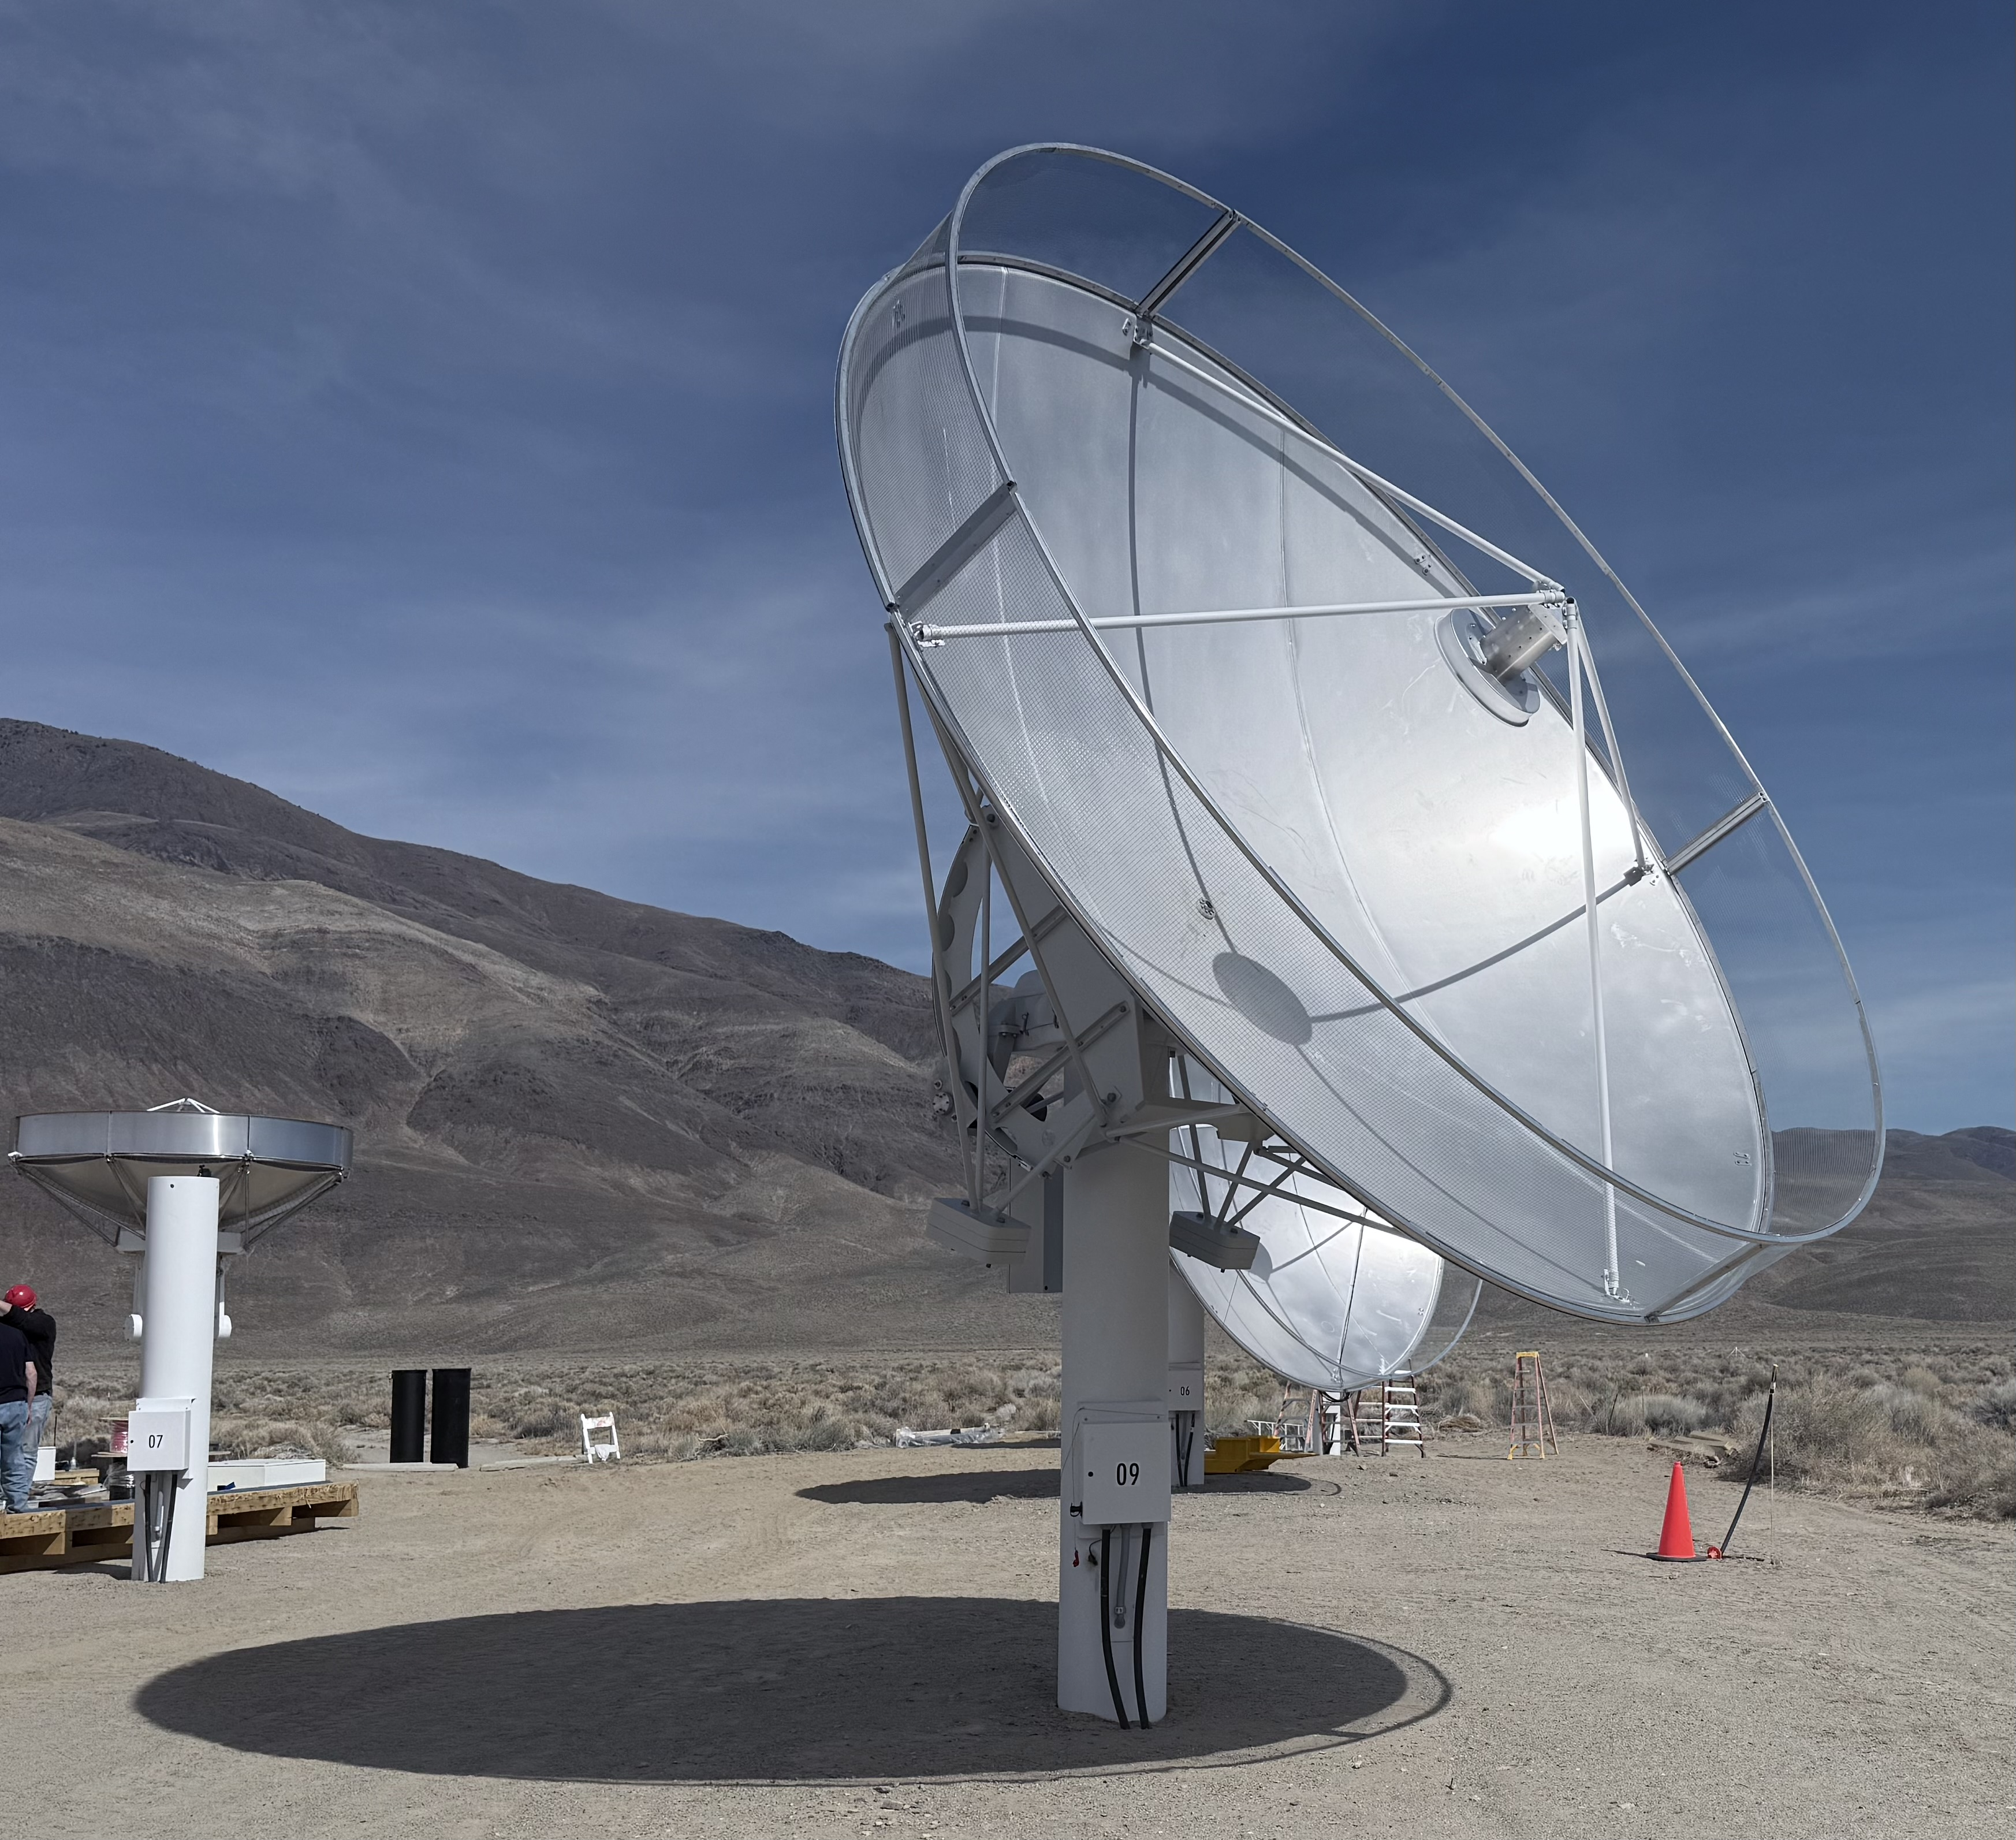
\includegraphics[width=\textwidth]{figures/test_array.jpg}
    \caption{DSA-2000 Test Array under construction at OVRO}
    \label{fig:test_array}
\end{figure}
\printbibliography[heading=subbibliography]
\end{refsection}

\chapter{Optimization of Low Noise Amplifiers} \label{ch:lna_opt}
\begin{refsection}
In this chapter, we discuss the analytic formalisms around the design of low noise amplifiers and applications in optimization-based design.
Too often, engineers quickly reach for the optimizer in the circuit simulator to achieve some desired result.
Without a sense of fundamental limits and a grasp on the trade-space, this can quickly lead to frustration when desired goals are not met.
All the trade-offs that we make when designing amplifiers are sourced from analytic expressions.
To design for a given point in the trade-space, we typically need to solve a nonlinear, constrained minimization problem.
For many of these optimization problems, the objective function is surprisingly convex\footnote{Where there is exactly one local minima, versus non-convex mathematical optimization which is generally NP-Hard}, with some having an exact, analytic solution.
We can use these solutions along with appropriate numerical optimization to quickly visualize the design space for a given device and make informed decisions during amplifier design.
This analytic background then provides motivation and bounds for building more complex amplifier optimization problems.

\section{Noise Theory Background}

No discussion around LNAs would be complete without an overview of noise in microwave circuits.
Rather than give full derivations, which can be found in many excellent textbooks, we will focus on the important results.

\subsection{Sources of Noise}

Johnson-Nyquist noise~\cite{nyquistThermalAgitationElectric1928} describes that a resistor at physical temperature $T$ produces a noise power proportional to its temperature due to the physical agitation of carriers inside the conductor.
For temperature $T$ and Boltzmann's constant $k_B$, the power spectral density of the noisy resistor is
%
\begin{equation}
    S_\text{Nyquist}~(W/\text{Hz}) = k_BT
    \label{eq:nyquist_noise}
\end{equation}
%
This noise power is approximately white, with the power spectral density falling off at high frequencies following Planck's law.
This approximation that $S_\text{Planck} \approx S_\text{Nyquist}$ is adequate up through terahertz frequencies at room temperature.
This noise is present in all electronics and can be the limiting factor in sensitivity at microwave frequencies.
As all sources of thermal noise are uncorrelated, there is little we can do to reduce it apart from physical cooling, motivating the use of cryogenics in applications such as radio telescopes and quantum computers.

Shot noise, described by Schottky in 1918~\cite{schottkyUberSpontaneStromschwankungen1918}, arises from random fluctuations in electric current due to the discretization of charge.
In DC conditions, if one were to observe each carrier individually pass through a conductor, the exact arrival time of the next carrier is uncertain and follows a Poissonian process.
We can compute the average velocity of the carriers, and this fluctuation in the actual count of carriers per unit time is the shot noise.
This process is also white, and given a current of $I$ and electron charge $q$, shot noise has a power spectral density of
\begin{equation}
    S_\text{Shot}~(A^2/\text{Hz}) = 2qI
    \label{eq:shot_nosie}
\end{equation}

Other sources of noise include $1/f$ noise which combines many mechanisms with a $1/f$ power spectral density and quantum noise which describes the minimum noise from a physical linear amplifier.
For microwave circuits, these sources of noise are usually dwarfed by thermal and shot noise.
The one exception here is for oscillators, however, as upconversion of $1/f$ noise can result in phase noise.

\subsection{Noise in Two Port Networks}

\begin{figure}[ht!]%
    \centering
    \subfloat{\includestandalone[mode=buildnew]{figures/noisy_abcd.tex}}%
    \quad%
    \subfloat{\includestandalone[mode=buildnew]{figures/noiseless_abcd.tex}}%
    \caption{Equivalent noise representations of ABCD networks}%
    \label{fig:noise_equiv_abcd}%
\end{figure}

Given a linear two port network with a collection of internal noise generators, Rothe and Dahlke show us in \cite{rotheTheoryNoisyFourpoles1956} that we can represent this circuit as a noiseless two port network with external, correlated noise generators.
\autoref{fig:noise_equiv_abcd} shows the equivalent circuits in an ABCD (cascade) network form, with the noise current and voltage sources at the input.
These sources are correlated by some complex correlation coefficient, $\rho$.
Given the magnitude of these noise sources and the correlation coefficient, one can draw a few conclusions about the behavior under varied source terminations.
For example, if the sources were perfectly correlated, we could present a source admittance $Y_S$ that will generate a noise voltage from $i_n$ to perfectly destructively interfere with $v_n$, resulting in zero noise.
As we have seen earlier, there are many uncorrelated noise processes in real circuits, so in reality this correlation in the input-referred noise generators is some nonzero, less than unity, quantity.
This, however, still implies that there exists a source impedance that minimizes the input-referred noise.

The noise dependence on the source admittance is the primary result that enables the development of low noise microwave amplifiers.
Just as we can design matching networks to power match devices, we can design matching networks to present the optimal source that minimizes noise.

\section{Noise Circles and Constraint Equations}

The noise figure of a two-port amplifier~\cite{gonzalezMicrowaveTransistorAmplifiers1997} is
%
\begin{equation}
    F = \FMin + \frac{4r_n|\GS - \GOpt|^2}{(1-|\GS|^2)|1+\GOpt|^2}
    \label{eq:noise_f}
\end{equation}
%
where $\FMin$ is the minimum achievable noise temperature, $r_n$ is the so-called noise equivalent resistance representing how quickly the noise changes as $\GS$ moves from $\GOpt$, normalized to the characteristic impedance $Z_0$, $\GOpt$ is the source reflection coefficient that achieves $\FMin$ and $\GS$ is the true source reflection coefficient.
These three numbers, $\FMin$, $r_n$, and $\GOpt$, form the noise parameters of an amplifier and fully characterize the noise behavior of the device under any source impedance condition.
If we were to attempt to solve this equation for $\GS$ such that we achieve a desired noise figure $F$, we start by separating the $\GS$ components from the rest of the equation
%
\begin{equation}
    \frac{|\GS-\GOpt|^2}{1 - |\GS|^2} = \frac{F - \FMin}{4r_n}|1 + \GOpt|^2
\end{equation}
%
As the right side of this equation is constant, we can write
%
\begin{equation}
    N = \frac{\Delta F}{4r_n}|1 + \GOpt|^2
    \label{eq:noise_N}
\end{equation}
%
where $\Delta F$ is the desired noise penalty (in noise figure) from $\FMin$.
Interestingly, the solution to this in $\GS$ is a circle on the complex plane with center
%
\begin{equation}
    C_F = \frac{\GOpt}{1 + N}
\end{equation}
%
and radius
\begin{equation}
    R_F = \frac{\sqrt{N^2+N(1-|\GOpt|^2)}}{1 + N}
\end{equation}
%
So, for a given set of noise parameters and desired noise (greater than or equal to the device's minimum noise), we can draw a circle on the Smith chart of equal noise.
If we were to design a matching network to build an amplifier for this noise, we have an infinite number of impedances to choose from.

As engineering is all about tradeoffs, we need to start introducing additional constraints apart from noise.
If we did not, one would rightly ask, "Why not simply match to $\GOpt$?"
Primarily, the answer to this arises from the unfortunate reality that $\GOpt$ is distinct from the actual conjugate input reflection coefficient of the device, $\GIn^*$.
This implies that as you attempt to match a device for optimum noise, you do not optimally deliver power to it.
In other words, the optimum noise impedance has a reflection or gain penalty.

In system design, these various performance metrics describe the trade-space.
One can pick high gain or low reflection, but have bad noise performance, or vice versa.
As Friis tells us in the cascaded noise equation~\cite{pozarMicrowaveEngineering2012}
%
\begin{equation}
    F_\text{Total} = F_1 + \frac{F_2 - 1}{G_{A_1}} + \frac{F_3 - 1}{G_{A_1}G_{A_2}} \dots + \frac{F_N-1}{\prod_{i=1}^{N-1}G_{A_i}}
\end{equation}
%
where $G_{A_i}$ is the available gain of the ith amplifier, we must maximize the gain of the early stages to reduce the noise impact of noise contributors further down the signal chain.
Again, part of the system design work is evaluating all these tradeoffs.

Traditionally, the exploration into these tradeoffs is rather brute-force.
However, a more disciplined approach can be taken.
We can formulate exact solutions for optimum noise under constraints, allowing us to explore theoretical limits given a device's intrinsic behavior and informing engineering decisions made in design.

\subsection{Optimum Noise Under Constraints}

Suppose we want to design an LNA with a given reflection coefficient or equivalent VSWR.
The amplifier we want will have minimum noise with VSWR being constant.
Given that:
%
\begin{equation}
\text{VSWR} = \frac{1+|\GA|}{1 - |\GA|}
\end{equation}
%
and
\begin{equation}
    |\GA| = \left|\frac{\GIn - \GS^*}{1 - \GIn \GS}\right|
    \label{eq:mga}
\end{equation}
%
where
%
\begin{equation}
    \GIn = S_{11} + \frac{S_{12}S_{21}\GL}{1-S_{22}\GL}
    \label{eq:gamma_in}
\end{equation}
%
we could write this problem as a mathematical minimization equation via
%
\begin{mini}
	{\GS}{F(\GS)}
	{}{}
	\addConstraint{|\GA|}{\leq|\GA|_\text{Max}}
    \label{eq:noise_mini}
\end{mini}
%
As written, this is a constrained, nonlinear optimization problem.
These kinds of problems are characteristically difficult to solve and are usually non-convex.
In this case, however, there is an exact solution.

In the previous section, we mentioned that constant noise induces circles in the $\GS$ plane.
The same is true for constant VSWR.
For a given $|\GA|$, we can draw the circle with center
%
\begin{equation}
    C_V = \frac{\GIn^*(1-|\GA|^2)}{1 - |\GA\GIn|^2}
\end{equation}
and radius
%
\begin{equation}
    R_V = \frac{\left||\GA||1-|\GIn|^2\right|}{\left|1-|\GA\GIn|^2\right|}
\end{equation}
%
Points inside this circle have strictly lower reflection, so we know a solution to \autoref{eq:noise_mini} must lie on this circle or inside it.
If we consider the case where $\GOpt$ is not inside the constant VSWR circle, we can fully constrain the optimum solution to lie on this circle.
This is where we apply the noise circle formalism from before.
As the radius of this circle scales with $\Delta F$, we want to find the noise circle that just touches the constant VSWR circle.
We know this will have a solution, as we can keep increasing the radius until it touches the VSWR circle.
We also know that this will have exactly one solution, as any further intersections would arise from a larger circle with higher noise.
This is the geometric intuition for the convexity of \autoref{eq:noise_mini}.

Expressing this condition mathematically, we can state
%
\begin{equation}
    R + R_F = |C-C_F|
\end{equation}
%
or the sum of the two circles' radii equal the Euclidean distance between the centers of the two circles, given an arbitrary circle with center $C$ and radius $R$ and the noise circle stated above.
Solving this relation for $N$ (\autoref{eq:noise_N}) gives the quadratic result following~\cite{linkAnalyticalExpressionsSimplifying1995}
%
\begin{equation}
    N = \frac{-B\pm\sqrt{B^2-4AC}}{2A}
    \label{eq:min_n_touch}
\end{equation}
%
where
\begin{align*}
    c_1 &= |C|^2 - R^2 - 1 \\
    c_2 &= |\GOpt-C|^2 - R^2 \\
    A &= c_1^2 - 4R^2 \\
    B &= 2c_1c_2 + 4R(|\GOpt|^2 - 1) \\
    C &= c_2^2
\end{align*}
%
We can then take this result and plug it in to \autoref{eq:noise_N} to solve for $\Delta F$.
To disambiguate between the two solutions, we apply the constraint that $N$ must be positive, and if both solutions are positive, we take the smaller of the two.
From here, we can immediately compute a minimum theoretical noise under a VSWR constraint.

\subsection{Worked Examples}
To showcase these results, we will be investigating the \qty{400}{\nm} x \qty{200}{\um} gate, four-finger (4F50) transistor from Diramics~\cite{DiramicsPH2004F50} at a bias of $V_d$=\qty{0.5}{\V}, $I_d$=\qty{16}{\mA}, using the vendor-supplied model.
To begin investigating this device, we can look at its S and noise parameters, with no further circuitry.
This allows us to set the stage for input/output matching and feedback.

\begin{figure}[ht!]%
    \centering
    \subfloat{\includestandalone[mode=buildnew]{figures/4f50_s_gopt}}%
    \quad%
    \subfloat{\includestandalone[mode=buildnew]{figures/4f50_gain}}%
    \caption{{4F50 $S_{11}$, $S_{22}$, $S_{21}$, and $\GOpt$ from \SIrange{0.1}{10}{\GHz}}}%
    \label{fig:4f50_s_gopt}%
\end{figure}

We can start by analyzing this device at a single frequency point, \qty{1.5}{\GHz}.
If we wanted the optimum $\GS$ for this device under the constraint that $|\GA| \leq 0.9$, we find $\Delta F$ of \qty{0.012} or an $F$ of \qty{1.038} or \qty{11.1}{\K} of noise temperature.
Using this result, we can compute the center and radii of the two circles.
Then, with both centers and either radius, we can compute their osculation point using simple geometry
%
\begin{equation}
    \GS =  
    \begin{cases}
        C_F - R_F\frac{C-C_F}{|C-C_F|},& \text{if\enspace}|C-C_F|\leq R \text{\enspace and\enspace} R_F\leq R\\
        C_F + R_F\frac{C-C_F}{|C-C_F|},              & \text{otherwise}
    \end{cases}
\end{equation}
%

Plotted on the Smith chart, we can see the result is as expected, with the intersection of the two circles giving the optimum $\Gamma_S$
\begin{figure}[ht!]
    \centering
    \includestandalone[mode=buildnew]{figures/mga_opt}
    \caption{$|\GA|$=0.9 optimum noise solution at \qty{1.5}{\GHz}}
    \label{fig:mga_opt}
\end{figure}

We can now begin to explore some useful results.
First, we could compute the achievable noise given a range of VSWR constraints to quickly analyze the tradeoff between the two.
In \autoref{fig:nf_vs_mga}, we plot the achievable noise temperature in K under a reflection constraint sweeping $|\GA|$ from 0.1 to 0.95.
A value for $|\GA|$ higher than 0.95 places $\GOpt$ inside the VSWR circle, implying that for any constraint higher than 0.95 we would pick $\GS$ = $\GOpt$ and our noise would be $\FMin$.
%
\begin{figure}[ht!]
    \centering
    \includestandalone[mode=buildnew]{figures/nf_vs_mga}
    \caption{Optimum noise figure versus $|\GA|$ at \qty{1.5}{\GHz}}
    \label{fig:nf_vs_mga}
\end{figure}
%
This result alone tells us that we will have to make major sacrifices in reflection to achieve good noise performance.

Another result from \autoref{eq:min_n_touch} is the fact that this solution is agnostic to the constraining circle.
Instead of VSWR, we could use a different circle such as constant gain instead.
Specifically, we would look at circles of constant available gain, as those are drawn in the $\GS$ plane as is noise.

Recall that available gain is defined as
%
\begin{equation}
    G_A = \frac{P_\text{AVN}}{P_\text{AVS}} = \frac{\text{Power available from the network}}{\text{Power available from the source}}
\end{equation}
%
where
%
\begin{equation}
    G_A = \frac{1-|\GS|^2}{|1-S_{11}\GS|^2}\frac{|S_{21}|^2}{1-|\GOut|^2}
    \label{eq:available_gain}
\end{equation}
%
and
%
\begin{equation}
    \GOut = S_{22} + \frac{S_{12}S_{21}\GS}{1-S_{11}\GS}
    \label{eq:gamma_out}
\end{equation}
%
This function is only parameterized by $\GS$ and the device characteristics, operating under the assumption that the output is conjugate-matched.
In the same manner as $\GA$ and noise, we can solve for the values of $\GS$ that result in the same available gain.
If we define a normalized desired gain of
%
\begin{equation}
    g_a = \frac{G_a}{|S_{21}|^2}
\end{equation}
%
the center and radius of the circles for constant $g_a$ are
%
\begin{equation}
    C_a = \frac{g_a\left(S_{11}^*-S_{22}\Delta^*\right)}{1 + g_a\left(\left| S_{11}\right|^2 - |\Delta|^2\right)}
\end{equation}
%
and
%
\begin{equation}
    R_a = \frac{\sqrt{
    1-g_a\left(1-|S_{11}|^2-|S_{22}|^2 + |\Delta|^2\right) + g_a^2|S_{12}S_{21}|^2
    }}
    {1 + g_a\left(\left| S_{11}\right|^2 - |\Delta|^2\right)}
\end{equation}
%
where
%
\begin{align*}
    \Delta &=S_{11}S_{22} - S_{12}S_{21}
\end{align*}

Looking back at \autoref{fig:4f50_s_gopt}, at \qty{1.5}{\GHz}, we have a maximum stable gain (MSG) of about \qty{25}{\dB} and an $S_{21}$ (gain under \qty{50}{\ohm} conditions) or about \qty{20}{\dB} where
%
\begin{equation}
    MSG = \frac{|S_{21}|}{|S_{12}|}
    \label{eq:msg}
\end{equation}
%
If we draw the circle of constant available gain of \qty{20}{\dB} (which intersects the center of the Smith chart, as it is the value of $S_{21}$) and the intersecting minimum noise circle, we get the result shown in \autoref{fig:gain_noise_opt}.
Notably, $\GOpt$ is inside the constant gain circle, implying that $\GOpt$ results in a higher gain than the chosen value.
While usually we would want more gain, we will proceed with the $G_A=$\qty{20}{dB} solution for illustration purposes.

\begin{figure}[ht!]
    \centering
    \includestandalone[mode=buildnew]{figures/gain_noise_opt}
    \caption{\qty{20}{\dB} optimum noise solution at 1.5 GHz}
    \label{fig:gain_noise_opt}
\end{figure}

Looking at the relative positions of $S_{11}^*$ and the VSWR circles from \autoref{fig:mga_opt}, this $\GS$ solution will have suboptimal VSWR.
To be more precise, we can plug this $\GS$ into \autoref{eq:mga} and find that the $|\GA|$ for this solution is \num{0.986} with a noise temperature of \qty{13.2}{\K}.
From the other perspective, if we took the $\GS$ solution from \autoref{fig:mga_opt} with a $|\GA|$ = 0.9, we find the available gain using \autoref{eq:available_gain} has a high negative value, indicating this solution is unstable!
If we use the unilateral approximation here where $S_{12}$ = 0, we will find that the available gain for the $\GS$ solution under the $|\GA|$ = 0.9 constraint is \qty{28}{\dB}, \qty{2}{\dB} over the maximum stable gain.
In fact, if we compute $\GOut$ for this same $\GS$, we find a magnitude greater than unity, indicating oscillation.

\subsection{Stability and Degeneration}

Up to this point, we have failed to mention the impact of stability on the computed results.
As we intend to design an amplifier and not an oscillator, it is imperative that the magnitudes of our reflection coefficients are less than unity.
For a single gain element (transistor), one can use Rowlett's~\cite{rollettStabilityPowerGainInvariants1962} stability factor, K, to determine if the amplifier is stable.
%
\begin{equation}
    K = \frac{1-|S_{11}|^2-|S_{22}|^2 + |\Delta|^2}{2|S_{12}S_{21}|}
\end{equation}
%
When K is greater than unity and the magnitude of the determinant of the S matrix $|\Delta|$ is less than unity, the amplifier is unconditionally stable.
This considers potential matching on both the source and load side of the device.

While stability is critical, we can be a bit more lax than ``unconditional'' stability.
To expand on this, stability of every impedance over the load plane is not strictly required, as we will know precisely what the $\GL$ value will be (assuming we are conjugate matching).
On the input, we have a bit more to consider.
As shown earlier, we have a range of impedances that represent various trade-offs.
To make sure we are correctly comparing performance between options, those $\GS$ solutions must be stable.
Additionally, we have been operating under the assumption that this LNA will be attached to a \qty{50}{\ohm} source, which is not quite true.
If this were a product, one has no idea what source impedance the customer might try to attach the amplifier to.
For us in astronomy, the impedance of the feed antenna will attempt to match to \qty{50}{\ohm}, but will degrade out of band.
We need to ensure that over the range that the amplifier has gain (which is quite high for this high $f_t$ Diramics device), the presented source impedance does not cause the amplifier to oscillate.

Instead of evaluating unconditional stability, we can focus on the magnitude of the S parameters and the geometric stability factors~\cite{edwardsNewCriterionLinear1992}.
Specifically, we can look at $\mu^\prime$, which gives us the distance from the center of the Smith chart to the source-plane stability circle (the boundary of the impedance region that pushes the device into instability).
If this quantity is greater than unity, no impedance in the source plane will cause the amplifier to oscillate.
\begin{equation}
    \mu^\prime = \frac{1-|S_{22}|^2}{|S_{11}-S_{22}^*\Delta| + |S_{21}S_{12}|}
    \label{eq:mu_prime}
\end{equation}

There are many ways one could stabilize a potentially unstable amplifier.
Unfortunately, most of these methods degrade the amplifier's noise.
An alternative strategy is to use the common technique of inductive degeneration~\cite{lerouxDetailedStudyCommonSource2005}.
For the common-source amplifier we are investigating, this degeneration is realized as an inductor on the source terminal.
In implementation, this could be a transmission line, a bond wire, or a lumped component.

We can directly compute the modified S parameters of the transistor under degeneration.
The series-series feedback of the inductor attached to the source terminal is equivalent to the sum of the networks' Z parameters, shown in \autoref{fig:series_series}.
%
\begin{figure}[ht!]
    \centering
    \includestandalone[mode=buildnew]{figures/series_series}
    \caption{Series-Series feedback in Z parameters}
    \label{fig:series_series}
\end{figure}

Converting our S parameters to Z parameters with
%
\begin{equation}
    \mathbf{Z} = \frac{Z_0}{\Delta_s}
    \begin{bmatrix}
    (1+S_{11})(1-S_{22})+S_{12}S_{21} & 2S_{12} \\
    2S_{21} & (1-S_{11})(1+S_{22})+S_{12}S_{21}
    \end{bmatrix}
    \label{eq:s2z}
\end{equation}
%
where
%
\begin{equation*}
    \Delta_s = (1-S_{11})(1-S_{22})-S_{12}S_{21}
\end{equation*}
and
%
\begin{equation}
    \mathbf{S} = \frac{1}{\Delta_z}
    \begin{bmatrix}
    (Z_{11}-Z_0)(Z_{22}+Z_0)+Z_{12}Z_{21} & 2Z_0Z_{12} \\
    2Z_0Z_{21} & (Z_{11}+Z_0)(Z_{22}-Z_0)-Z_{12}Z_{21}
    \end{bmatrix}
    \label{eq:z2s}
\end{equation}
%
where
%
\begin{equation*}
    \Delta_z = (Z_{11}+Z_0)(Z_{22}+Z_0)-Z_{12}Z_{21}
\end{equation*}
%
we can take our device's S parameters, convert to Z parameters, add the Z parameters of the impedance of the feedback ($ZJ_2$ where $J_2$ is the 2x2 unit-matrix), and convert back to S parameters to evaluate the new S parameters and derived stability.
The S parameters of this construction are
%
\begin{equation}
    \mathbf{S}_\text{Degen} = \frac{1}{Z(S_{11}+S_{12}+S_{21}+S_{22}) - 2Z_0}\left(\begin{bmatrix}
        \Delta_A & \Delta_B \\
        \Delta_B & \Delta_A
    \end{bmatrix}
    +
    2Z_0\mathbf{S}
    \right)
    \label{eq:s_degen}
\end{equation}
%
where
%
\begin{align*}
    \Delta_A &= \Delta + S_{12}+S_{21} - 1 \\
    \Delta_B &= -\Delta + S_{11}+S_{22} - 1
\end{align*}

We could attempt to plug in \autoref{eq:s_degen} to \autoref{eq:mu_prime} and solve for the L that forces $\mu^\prime$ to unity, but we are unfortunately not guaranteed a solution.
A better approach is to plot $\mu^\prime$ across a range of inductances to explore the trade space.
However, the maximum gain of the modified amplifier also changes with degeneration, as expected for an amplifier under feedback.
These two metrics are plotted versus the degeneration inductance in \autoref{fig:L_msg_degen}.
%
\begin{figure}[ht!]%
    \centering
    \subfloat{\includestandalone[mode=buildnew]{figures/L_degen}}%
    \quad%
    \subfloat{\includestandalone[mode=buildnew]{figures/msg_degen}}%
    \caption{$\mu^\prime$ and MSG versus inductive degeneration for the 4F50 at \qty{1.5}{\GHz}}%
    \label{fig:L_msg_degen}%
\end{figure}

From these results, we can determine that to achieve an MSG of \qty{20}{\dB}, we can tolerate at most \qty{1.5}{\nH} of degeneration.
The $\mu^\prime$ metric tells us the distance of the source stability circle from the center of the Smith chart, so we can compare this value with the magnitude of the desired $\GS$ to evaluate conditional stability.
\qty{1.5}{\nH} is a reasonable value, as we will be wire bonding the source pad of the die transistor, and the rule of thumb is about \qty{1}{\nH} of inductance per \qty{1}{\mm} of bond wire length.

Next, we must evaluate the effect of the degeneration on the noise parameters.
Starting from the Hartmann and Strutt result~\cite{hartmannChangesFourNoise1973} which describes the changes in noise parameters under feedback, we can compute the ``noise parameter transformation matrix'' as
%
\begin{equation}
    n = \frac{1}{\Delta_n}\begin{bmatrix}
        \Delta_n &  Z_0Z(\Delta + S_{22}-S_{11}+2S_{21}-1) \\
        0 & 2S_{21}Z_0
    \end{bmatrix}
\end{equation}
%
where
%
\begin{equation*}
    \Delta_n = Z(S_{11}-1)(S_{22}-1) + S_{21}(2Z_0-S_{12}Z)
\end{equation*}
%
under the assumption of series feedback, as is the case for the degeneration inductance as shown earlier.
From here, we use the relations
%
\begin{align}
    R_n^\prime &= R_n|n_{11} + n_{12}Y_\text{Corr}|^2 + G_n|n_{12}|^2 \\
    G_n^\prime &= \frac{G_nR_n|n_{11}n_{22} - n_{12}n_{21}|^2}{R_n^\prime} \\
    Y_\text{Corr}^\prime &= \frac{R_n(n_{21} + n_{22}Y_\text{Corr})(n_{11}^*+n_{12}^*Y_\text{Corr}^*) + G_nn_{22}n_{12}^*}{R_n^\prime}
\end{align}
%
where $R_n$ is the same noise resistance, $G_n$ is the noise conductance, and $Y_\text{Corr}=G_\text{Corr}+jB_\text{Corr}$ is the correlation admittance, with the noise figure equation here being expressed as
%
\begin{equation}
    F = 1 + \frac{G_n}{G_s} + \frac{R_n}{G_s}|Y_S - Y_\text{Corr}|^2
\end{equation}
%
with $Y_S=G_S+jB_S$ being the source admittance.
This is a separate form of the noise equation from \autoref{eq:noise_f}, and we can convert between the two using results from \cite{heymannNoiseLinearTwoPorts2022} with
%
\begin{align}
    Y_\text{Opt} &= \sqrt{\frac{G_N}{R_N}+G_\text{Corr}^2} - jB_\text{Corr} \\
    \FMin &= 1 + 2R_N(G_\text{Corr} + G_\text{Opt})
\end{align}
%
and
%
\begin{align}
    Y_\text{Corr} &= \frac{\FMin - 1}{2R_N} - G_\text{Opt} - jB_\text{Opt} \\
    G_N &= R_N(G_\text{Opt}^2 - G_\text{Corr}^2)
\end{align}
%
With this result, we can recompute the noise behavior of the degenerated device.
With this small inductance, the resulting noise parameters do not change much.
\cite{hartmannChangesFourNoise1973} gives an approximation that under the conditions
\begin{equation}
    L_\text{Degen} \ll \frac{1}{\omega}\left| \frac{2S_{21}Z_0}{(1-S_{11})(1-S_{22})-S_{12}S_{21}} \right|
\end{equation}
and
\begin{equation}
    \Re\{n_{12}\} \ll \frac{R_n\Re\{Y_\text{Corr}\}}{R_n|Y_\text{Corr}|^2+G_n}
\end{equation}
the noise parameters are practically unchanged.
We will, however, not make this assumption.
The degenerated S parameters and $\GOpt$ are shown in \autoref{fig:4f50_s_gopt_mga_degen} along with the optimum noise $\GS$ under a \qty{20}{\dB} gain constraint, similar to \autoref{fig:gain_noise_opt}.
%
\begin{figure}[ht!]%
    \centering
    \subfloat{\includestandalone[mode=buildnew]{figures/4f50_s_and_gopt_degen}}%
    \subfloat{\includestandalone[mode=buildnew]{figures/mga_opt_degen}}%
    \caption{$S_{11}$, $S_{22}$, and $\GOpt$ from \SIrange{0.1}{10}{\GHz} and noise optimum $\GS$ at \qty{1.5}{\GHz} under \qty{1.5}{\nH} source degeneration}%
    \label{fig:4f50_s_gopt_mga_degen}%
\end{figure}

While this result looks similar to \autoref{fig:mga_opt}, this $\GS$ solution achieves a noise temperature of \qty{9.56}{\K} with a $|\GA|$ of only \num{0.195}, or an $|S_{11}|^2$ of \qty{-14.2}{\dB}, which is quite impressive for an LNA.

If this were a single-frequency design, we could design a simple matching network to conjugate-match the output and provide the $\GS$ solved here at the input.
Much to the chagrin of the RF engineer, customers and scientists demand bandwidth.
Next, we will explore how these design techniques apply to wideband design.

\section{Wideband Design Under Constraints}

Using the techniques established thus far, we can begin to evaluate the wideband behavior of the transistor under investigation.
To do so, we can solve either the VSWR or gain constrained problem, and plot the resulting noise, gain, and $S_{11}$ versus frequency.
For this section, we will focus on the same device and bias point, over the \SIrange{0.7}{2}{\GHz} range, matching the target band for the DSA-2000.

We will begin by choosing a desired gain constraint, $G_A$\qty{=20}{\dB}.
We then evaluate MSG over frequency and degeneration inductance to find what maximum degeneration value allows for an MSG greater than our desired $G_A$ across the band.
We are maximizing degeneration to result in a maximally stable amplifier.
The plot of MSG versus frequency and degeneration is shown in \autoref{fig:msg_freq_l}.
From this result, we can see that to achieve \qty{20}{\dB} of gain over our entire frequency range, we need an inductance of \qty{0.8}{\nH}, less than our \qty{1.5}{\nH} result from before.
%
\begin{figure}[ht!]
    \centering
     \includestandalone[mode=buildnew]{figures/msg_freq_l}
    \caption{MSG vs Degeneration vs Freq}
    \label{fig:msg_freq_l}
\end{figure}

With this degeneration value, we can solve for the optimum noise $\GS$ under a $G_A$\qty{=20}{\dB} constraint, and compute the remaining parameters such as the input and output return loss and noise.
%
\begin{figure}[ht!]
    \centering
     \includestandalone[mode=buildnew]{figures/_08nh_20db}
    \caption{Performance under \qty{0.8}{\nH} degeneration with a \qty{20}{\dB} gain constraint}
    \label{fig:_08nh_20db}
\end{figure}

In \autoref{fig:_08nh_20db}, we can see that from \SIrange{0.7}{1.75}{\GHz}, we can achieve higher gain than the requested value, with $\GS$ taking on $\GOpt$.
After this point, however, we sacrifice noise to maintain our gain requirement.
Additionally, looking at the input return loss (IRL) and output return loss (ORL), we see they are reasonable values, notably positive (in loss) indicating this implementation is stable, as we expect from the MSG curve.
However, at \qty{2}{\GHz} we are right at the limit of stable gain under the gain matching condition.
This may imply that small perturbations in the design will cause it to oscillate.
To build a more robust amplifier, we will want additional margin.
Furthermore, the noise gets significantly worse past \qty{1.75}{\GHz}.
\newpage

\begin{figure}[ht!]
    \centering
     \includestandalone[mode=buildnew]{figures/_08nh_18db}
    \caption{Performance under \qty{0.8}{\nH} degeneration with a \qty{18}{\dB} gain constraint}
    \label{fig:_08nh_18db}
\end{figure}

With the same degeneration value, we can look at a slightly loosened gain constraint of \qty{18}{\dB}.
Shown in \autoref{fig:_08nh_18db}, we see that we are meeting our gain requirement across the whole frequency range, implying the optimum $\GS$ is simply $\GOpt$.

For radio astronomy, we aren't particularly interested in the various return losses, rather gain and noise.
Noise, of course, gives the telescope sensitivity, while gain reduces the impact of the noise generators after the LNA.
We could look at the noise performance under return loss constraints, but we would see similar results as this exercise with gain.
As such, we can move our attention to the implementation of the network that performs the match to $\GOpt$.

\section{Wideband Nonuniform Line Matching}

From the result in \autoref{fig:_08nh_18db}, we know now we want to create a matching network directly for $\GOpt$, under \qty{0.8}{\nH} of inductive source degeneration.
Unfortunately, there is not an analytic way to design a matching network for an arbitrary impedance response with frequency.
There are many optimization approaches in the literature, perhaps the most popular being the ``Real Frequency Technique''~\cite{yarmanSimplifiedRealFrequency1982,carlinOptimumBroadbandMatching1981}.
In this approach, coefficients for a Laplace-domain polynomial are optimized, minimizing an error function between desired behavior and modelled in the least-squares sense.
Solving for these polynomials involves iterative root-finding, on top of the normal iterative gradient-descent optimization.
After we have found the optimum $N$th order polynomial, we still need to perform a synthesis step where we transform the result into lumped or distributed components.
Unfortunately, there is no guarantee during optimization that the resulting implementation is physical.
Additionally, the multistep iteration and finite-difference approximation of the gradient is slow and imprecise.

If we happened to know the topology of the matching network a priori, we could attempt to directly optimize it using the same least-squares approach.
For the case of this amplifier we are attempting to design, there are very few matching topologies which would be acceptable.
This primarily comes from the fact that $\FMin$ is so low, so any discrete components will be much too lossy and significantly impact our noise.
So, we are left with transmission line matching, either as cascaded stubs, cascaded steps, or some combination of the two.
One of the more interesting topologies to investigate is the nonuniform transmission line (NTL).
These lines vary their impedance continuously as a function of position.
NTLs have been widely studied in matching contexts, even for complex loads~\cite{xiaoImpedanceMatchingComplex2002}.

Here, we can attempt to use NTLs to match to $\GOpt$ over our wide bandwidth, formulated as a least-squares problem against $\GS$.
The difficulty, however, is parameterizing the NTL in a simple way that allows us to compute $\GS$.
A common approach is to discretize the line into many uniform sections and cascade their scattering behavior.
With many sections, this yields a good approximation to the smooth transmission line.

In optimization, we will use a gradient-descent approach, which will require the derivative of our cost function with respect to every input variable.
If we parameterize the NTL by $N$ lines of characteristic impedance $Z_i$, each with constant length of $\delta L$ across $M$ distinct frequencies $\nu$ and source reflection coefficient (before this input matching network) of $\GS$, we can write a cost function as
%
\begin{equation}
    E = \frac{1}{M}\sum_{i=1}^M \left| \Gamma_\text{Out}\left(\prod_{j=1}^N A(Z_j,\delta L, \nu_i),\Gamma_S\right) - \Gamma_{\text{Opt}_i} \right|^2
    \label{eq:tline_cost}
\end{equation}
%
where the final ABCD parameters can be converted to S parameters using the standard transformations~\cite{pozarMicrowaveEngineering2012}.
As all the expressions thus far are analytic, the gradient for $\delta E/\delta Z_j$ has an analytic form.
As $N$ increases, however, this expression will have exponentially more terms.
One could use the finite-difference method to compute this derivative, but this is inefficient and imprecise.
Instead, we will make use of automatic differentiation to compute the exact gradients.
There are significant performance implications here, which will be discussed in \autoref{ch:lna}.

One interesting note about the cost function in \autoref{eq:tline_cost} is that we will minimize geometric error to $\GOpt$, not noise.
The distance between $\GS$ and $\GOpt$ is proportional to noise, but the true relationship follows from \autoref{eq:noise_f}, which contains the same geometric error term of $|\GS - \GOpt|^2$, but is divided by $1-|\GS|^2$.
We could use the full noise equation in optimization, however this more simple geometric approximation yielded a satisfactory result.

Given a set of $\GOpt$ with frequency and a total length $L$, we can compute the optimum $Z_j$ versus linear distance profile.
In the current formulation, the total length of the line $L$ is not part of the optimization, so we must pick a few lengths to see the response surface.
From\cite{xiaoImpedanceMatchingComplex2002}, longer lines should yield better results, although we will be at odds with insertion loss in actual implementation.
We can start our investigation with length using slightly less than $\lambda/4$ at \qty{700}{\MHz}, as NTLs have been used for miniaturization of quarter wave lines before\cite{khalaj-amirhosseiniNonuniformTransmissionLines2008}.
In free space, we will start at \qty{80}{\mm} and test various lengths.
We will also constrain the characteristic impedances between \qty{45}{\ohm} and \qty{350}{\ohm} as that is the range of what is practically realizable in suspended microstrip.
The resulting profile and performance is shown in \autoref{fig:l80_lambda0}.
%
\begin{figure}[ht!]%
    \centering
    \subfloat{\includestandalone[mode=buildnew]{figures/l80_lambda0_profile}}%
    \quad%
    \subfloat{\includestandalone[mode=buildnew]{figures/l80_lambda0_t_g}}%
    \caption{Optimal impedance profile, noise, and gain for an \qty{80}{\mm} NTL}%
    \label{fig:l80_lambda0}%
\end{figure}

In \autoref{fig:l80_lambda0}, a few things are immediately apparent.
One, the line is notably not smooth at all, rather oscillating between the high and low impedance limits.
The noise match, however, is quite reasonable, with a band-average of \qty{7.99}{\K} compared to the band-average of $T_\text{Min}$ of \qty{7.64}{\K}.
Unfortunately, the sharp discontinuities break our working assumption of smoothness in the nonuniform lines.
These discontinuities can create EM effects not captured by the cascaded uniform section model.
For example, in microstrip, large step discontinuities such as these can drastically alter circuit behavior and must be accounted for~\cite{edwardsDiscontinuitiesMicrostrip2016}.
This behavior of optimizing discrete shapes in NTLs has been seen before~\cite{miazgaDiscreteShapeOptimization2008} and in the limit approximates an R-transformer~\cite{rosloniecDesignSteppedTransmission1994}.
We have a few options to account for this.
One, we could add in a circuit model of the discontinuity, although this would rely on knowing the transmission line implementation.
Second, we could add a constraint to the optimization to account for smoothness.
We will choose the latter here, as we want to make minimal assumptions about the transmission line topology.

In~\cite{miazgaNonuniformTransmissionLine2014}, one option to contend with the stepped behavior of NTL optimization is to add a constraint where every impedance step is no more than some preset limit.
For a \num{100}-section line, this adds a \num{99}-element constraint vector, with an associated highly sparse constraint Jacobian.
This adds a lot of complexity to the optimization problem and makes the performance significantly worse.
We propose an alternative of simply regularizing for total smoothness by adding a Lagrange multiplier to the sum of impedance deltas.
With this, the new cost function looks like
%
\begin{equation}
    E = \frac{1}{M}\sum_{i=1}^M \left| \Gamma_\text{Out}\left(\prod_{j=1}^N A(Z_j,\delta L, \nu_i),\Gamma_S\right) - \Gamma_{\text{Opt}_i} \right|^2 + \frac{\lambda}{M} \sum_{i=2}^{M}\left|Z_i-Z_{i-1}\right|^2
    \label{eq:tline_cost_reg}
\end{equation}
%
where $\lambda$ adjusts the strength of the regularization term.

For the same $M$=100, L=\qty{80}{\mm} problem, but now with regularization for $\lambda$=\num{0.005}, we get the result shown in \autoref{fig:l80_lambda005}.
While this result is certainly smooth, the gain and noise profiles are worse.
The average noise temperature is now \qty{8.53}{\K}, about half a Kelvin worse than the previous result and \qty{1}{\K} worse than the minimum noise.
Lowering $\lambda$ improves this, but of course, with sharper features in the impedance profile.

The performance of the smooth line allows us to conclude that we may be better served with a longer line.
This agrees with~\cite{xiaoImpedanceMatchingComplex2002}, in that the longer line is similar to more cascaded transformers.
Using the same $\lambda$=0.005 regularization, we can re-run the optimization for a few different lengths shown in \autoref{fig:l80_lambda005}, \autoref{fig:l100_lambda005}, and \autoref{fig:l120_lambda005}.
The noise is decreasing with increased length, with the \qty{120}{\mm} design achieving \qty{7.90}{\K}, a bit better than the \qty{80}{\mm} unregularized solution.

All these smooth solutions are realizable in suspended stripline/microstrip, but we have failed to account for the insertion loss of the matching network itself.
As the line grows in length, so does its loss and therefore noise.
As the resulting design achieves a noise of \qty{10}{\K}, even \qty{0.15}{\dB} of insertion loss will double the noise.
Additionally, the loss of the line is roughly proportional to its impedance, so the more high impedance section line we have, the worse the noise due to the smaller cross-sectional area and associated resistance per unit length.
The precise details of optimizing the line considering its loss is the subject of \autoref{ch:lna}.

\section{Summary}

Using closed form expressions, we can quickly analyze the trade space of an amplifier design for a given transistor and its noise parameters.
Using formulas for gain or VSWR constrains, we can find theoretical limits on noise, available gain, and stability.
We apply these relations to every point in frequency to expand our understanding of the circuit in a wideband sense.
Finally, with an appreciation of these limits, we can move to optimization to realize the desired $\GS$ versus frequency.
The presented solution was a nonuniform line implementation of the noise matching network, but one could use a myriad of other matching techniques depending on the optimal $\GS$ curve desired.

\newpage
\begin{figure}[ht!]%
    \centering
    \subfloat{\includestandalone[mode=buildnew]{figures/l80_lambda005_profile}}%
    \quad%
    \subfloat{\includestandalone[mode=buildnew]{figures/l80_lambda005_t_g}}%
    \caption{Impedance profile, noise, and gain for an \qty{80}{\mm} NTL, $\lambda$=0.005}%
    \label{fig:l80_lambda005}%

    \subfloat{\includestandalone[mode=buildnew]{figures/l100_lambda005_profile}}%
    \quad%
    \subfloat{\includestandalone[mode=buildnew]{figures/l100_lambda005_t_g}}%
    \caption{Impedance profile, noise, and gain for an \qty{100}{\mm} NTL, $\lambda$=0.005}%
    \label{fig:l100_lambda005}%

    \subfloat{\includestandalone[mode=buildnew]{figures/l120_lambda005_profile}}%
    \quad%
    \subfloat{\includestandalone[mode=buildnew]{figures/l120_lambda005_t_g}}%
    \caption{Impedance profile, noise, and gain for an \qty{120}{\mm} NTL, $\lambda$=0.005}%
    \label{fig:l120_lambda005}%
\end{figure}
\newpage
\printbibliography[heading=subbibliography]
\end{refsection}

\chapter{Computationally Efficient Design of an LNA Input Matching Network Using Automatic Differentiation} 
\label{ch:lna}
\publishedas{shilaRapidDesignLNASubmitted}
\begin{refsection}
In this chapter, we present a method for the design of an LNA input matching network using automatic differentiation (AD), a technique made popular by machine learning.
The input matching network consists of a non-uniform suspended stripline transformer, directly optimized with AD-provided gradients.
Compared to the standard approach of finite-differences, AD provides orders of magnitude faster optimization time for gradient-based solvers.
This dramatic speedup reduces the iteration time during design and enables the exploration of more complex geometries.
The LNA designed with this approach improves over a previous two-section uniform-line design, achieving an average noise temperature of \newnoise over the frequency range of \qtyrange{0.7}{2}{\GHz} at room temperature.
We optimized the geometry in under \qty{5}{\s}, \num{40}x faster than optimizing with finite-differences.

\section{Introduction}

Radio telescope receivers are typically cooled to give high sensitivity, but the cost of cooling is prohibitive for arrays of thousands of telescopes.
Receivers with ambient-temperature LNAs are becoming competitive with cooled designs at low frequencies, resulting in dramatically decreased cost that enables the development of enormous arrays such as the DSA-2000~\cite{hallinanDSA2000RadioSurvey2019}.
A key metric for these arrays is the speed at which they create images of the sky.
The observation time required for some fixed noise in an image is $\propto T^2$, where $T$ is the system noise temperature.
At decimeter wavelengths, LNA noise typically dominates the system noise~\cite{flygareWidebandLowLossFeed2024}, so even \qty{1}{\K} improvement in the LNA significantly increases the survey speed and subsequent science return.
The key LNA development has been the use of a low-noise transistor from Diramics~\cite{DiramicsPH2004F50} with a low-loss suspended stripline input matching network~\cite{weinrebLowNoiseAmplifier2021, shiRoomTemperatureLowNoiseAmplifier2023}, consisting of uniform transmission line (UTL) transformers.
We have improved the LNA noise temperature by changing the input matching network to a non-uniform transmission line (NTL).

It is well known that NTLs are useful in wideband matching and are easily implemented in suspended stripline.
For our LNA, an NTL gives a better trade-off between insertion loss and noise match, but designing such a line is nontrivial.
The geometry must be directly optimized in situ, as no closed-form expression for the desired behavior of the NTL exists.

To optimize the geometry of the NTL, we follow the standard practice of gradient descent.
In most electronic design automation (EDA) packages, the gradient is approximated via finite-differencing, but finite-differencing is imprecise and inefficient for large-dimensional optimization, as is the case for an NTL problem.
While direct optimization is a common technique in designing NTLs~\cite{miazgaNonuniformTransmissionLine2014, miazgaDiscreteShapeOptimization2008, schaepperleOptimizationDistributedParameter1994}, the performance overhead of computing the gradient is a limiting factor.

Instead of computing the gradient with finite-differencing, we used automatic differentiation (AD)~\cite{baydinAutomaticDifferentiationMachine2017}, an algorithmic tool made popular by machine learning.
AD is an accelerated way to compute the exact derivatives of an arbitrary computer program.
As AD is an exact method, it is more precise than finite-differencing and typically higher performance.
Gradient-descent optimization of NTLs with AD dramatically reduces optimization time, which enables more complex designs.

In this chapter, we describe the design, implementation, and experimental verification of an LNA whose input matching network is an NTL designed via direct optimization using AD.
The NTL design achieves lower average noise temperature than the UTL design.
Optimization of the NTL took under \qty{5}{\s}, \num{40}x faster than solving the equivalent finite-differenced gradient-based problem in a commercial EDA package.

In \autoref{sec:math}, we discuss this mathematical formulation in detail with an overview of the LNA design problem posed as constrained nonlinear optimization, the AD method, and NTL design.
In \autoref{sec:impl}, we discuss the implementation details of applying this technique to our LNA design.
Finally, in \autoref{sec:measurement}, we present experimental results to demonstrate the performance of the amplifier.

\section{Mathematical Formulation} \label{sec:math}

\subsection{Low-Noise Amplifier Optimization}

The priority for any LNA design is to minimize the amplifier's noise.
Balancing this priority with other requirements such as input reflection, stability, gain, etc. is application-specific and is stated mathematically as
%
\begin{mini}
	{\GS}{F(\FMin, R_n, \GOpt, \GS)}
	{}{}
	\addConstraint{G(\mathbf{S}, \GL, \GS)}{\leq \xi}
	\label{eqn:optim}
\end{mini}
%
where $F$ is the noise objective function, given here in the standard form of noise figure~\cite{gonzalezMicrowaveTransistorAmplifiers1997}, driven by the device's noise parameters via
%
\begin{equation}
	F = \FMin + \frac{4R_{n}\left|\GS-\GOpt\right|^{2}}{Z_{0}\left|1+\GOpt\right|^{2}\left(1-\left|\GS\right|^{2}\right)}
	\label{eq:noise}
\end{equation}
%
where $\FMin$ is the minimum noise figure, $R_{n}$ is the noise equivalent resistance, and $\GOpt$ is the optimum source reflection coefficient that results in $\FMin$.
$G$ is the constraint, a function of the transistor's S parameters, $\mathbf{S}$, and input and output reflection coefficients, $\GS$ and $\GL$, shown in \autoref{fig:fet_gammas}.
The constraint function captures any of the non-noise requirements and is represented by an inequality with some scalar $\xi$.
The solution to \eqref{eqn:optim} is the $\GS$ that minimizes the noise figure given a biased transistor's S and noise parameters under some constraint.
Notably, the solution gives minimum noise without specifying any goal or target.
It is then up to the designer to evaluate the result and determine if it is satisfactory, loosening the constraints as necessary.
This is distinct from ``goal-based'' optimization, where the optimizer attempts to solve a potentially unfeasible problem and returns a goal-weighted least-squares solution.

If we were only interested in constraining input reflection, we would define $\xi$ as a maximum allowed magnitude of $\GA$ and write our constraint function as
%
\begin{equation}
	G \leq\left|\GA\right|_{\text{Max}}
	\label{eq:ga_constraint}
\end{equation}
Alternatively, we could constrain the gain to be greater than some value, either case being a trade-off between power and noise match.
In this work, we will constrain $|\GA|$.
%
\begin{figure}[t]
	\centering
	\begin{circuitikz}[european]
		\tikzstyle{every node}=[font=\LARGE]
		\draw (4.5,12.25) to[Tnmos] (4.5,14.25);
		\draw (3.65,13.25) to[short] (3.5,13.25);
		\draw  (1.5,14.5) rectangle (3,12);
		\draw  (5.25,14.5) rectangle (6.75,12);
		\draw [short] (4.5,14.25) -- (5.25,14.25);
		\draw [short] (3,12.25) -- (5.25,12.25);
		\draw (7.25,14) to[R] (7.25,12.5);
		\node [font=\small] at (7.25,13.25) {$Z_{L}$};
		\draw (3.5,13.25) to[short] (3.5,14.25);
		\draw (3.5,14.25) to[short] (3,14.25);
		\draw (1,14) to[R] (1,12.5);
		\node [font=\small] at (1,13.25) {$Z_{S}$};
        
		\node [font=\large] at (2.25,13.25) {IMN};
		\node [font=\large] at (6,13.25) {OMN};
        
		\draw [->, >=Stealth] (3.25,12.5) -- (3.5,12.5);
		\draw [short] (3.25,12.5) -- (3.25,12);
		\node [font=\small] at (3.25,11.75) {$\Gamma_{\text{In}}$};
        
		\draw [short] (5,12.5) -- (5,12);
		\draw [->, >=Stealth] (5,12.5) -- (4.75,12.5);
		\node [font=\small] at (5,11.75) {$\Gamma_{\text{Out}}$};
		\node [font=\small] at (1.25,11.75) {$\Gamma_{\text{A}}$};
		\node [font=\small] at (1.25,12.5) {};
		\draw [->, >=Stealth] (1.25,12.5) -- (1.5,12.5);
        
		\draw (1.25,12.5) to[short] (1.25,12);
		\draw [->, >=Stealth] (7,12.5) -- (6.75,12.5);
		\node [font=\small] at (7,11.75) {$\Gamma_{\text{B}}$};

        \draw [->, >=Stealth] (1.25,14) -- (1,14);
		\draw (1.25,14) to[short] (1.25,14.5);
		\node [font=\small] at (1.25,14.75) {$\Gamma_{\text{S}}$};
        
		\draw [->, >=Stealth] (3.25,14) -- (3,14);
		\draw (3.25,14) to[short] (3.25,14.5);
		\node [font=\small] at (3.25,14.75) {$\Gamma_{\text{S}}^\prime$};
        
		\draw [->, >=Stealth] (5,14) -- (5.25,14);
		\draw [short] (5,14) -- (5,14.5);
		\node [font=\small] at (5,14.75) {$\Gamma_{\text{L}}^\prime$};

        \draw [->, >=Stealth] (7,14) -- (7.25,14);
		\draw [short] (7,14) -- (7,14.5);
		\node [font=\small] at (7,14.75) {$\Gamma_{\text{L}}$};

        
		\draw [short] (7,12.5) -- (7,12);
		\draw (1,14) to[short] (1,14.25);
		\draw (1,14.25) to[short] (1.5,14.25);
		\draw (1,12.5) to[short] (1,12.25);
		\draw (1,12.25) to[short] (1.5,12.25);
		\draw (7.25,14) to[short] (7.25,14.25);
		\draw (6.75,14.25) to[short] (7.25,14.25);ragged
		\draw (6.75,12.25) to[short] (7.25,12.25);
		\draw (7.25,12.5) to[short] (7.25,12.25);
	\end{circuitikz}
	\caption{Reflection planes for a typical microwave transistor amplifier, its input matching network (IMN) and output matching network (OMN)}
	\label{fig:fet_gammas}
\end{figure}

The optimal $\GS$ solution, however, is only valid at a single frequency and could be readily solved by hand.
In practice, we sample the device's S and noise parameters across a set of $N$ discrete frequency points, $\nuvec$, and our goal is to design an amplifier that operates over a subset of that range.
For this wideband LNA design, one formulation is to minimize the average noise
%
\begin{mini}
	{\GS(\nuvec)}{\frac{1}{N}\sum_{i=1}^{N} F(\nu_i)}
	{}{}
	\addConstraint{G(\nuvec)}{\leq\left|\GA\right|_{\text{Max}}}
	\label{eqn:optim_geo}
\end{mini}
%
Here, the minimizer and constraints are vector-valued.
In this form, \eqref{eqn:optim_geo} is a constrained, weighted, nonlinear least-squares problem, as minimizing the average noise figure over $\GS(\nuvec)$ is proportional to minimizing the $R_n$-weighted mean squared distance between $\GS(\nuvec)$ and $\GOpt(\nuvec)$, subject to the input reflection constraint.

In practice, the $\GS(\nuvec)$ solution is not directly useful, as ultimately, we aim to design the network that induces $\GS(\nuvec)$.
Therefore, instead of minimizing over $\GS(\nuvec)$, we minimize over the input matching network directly.
If, for example, this matching network were a series UTL with electrical length $l$, phase constant $\beta$, and characteristic impedance $Z_L$, the problem becomes
\begin{mini}
	{l, Z_L}{\frac{1}{N}\sum_{i=1}^{N} F({\GS}(\nu_i))}
	{}{}
	\addConstraint{G({\GS}(\nuvec))}{\leq\left|\GA\right|_{\text{Max}}}
	\label{eqn:optim_line}
\end{mini}
%
where
\begin{equation}
	\GS(\nu) = Z_0\left[\frac{Z_L +jZ_0\tan\left(\beta(\nu)l\right)}{Z_0 +jZ_L\tan\left(\beta(\nu)l\right)}\right]
\end{equation}
%
Here, we reduce the dimensionality of the problem from $N$ to two as we are solving for a single length and characteristic impedance.
However, there is no guarantee that this topology achieves the same average noise figure as the optimum $\GS(\nuvec)$ solution.
Solving this transformed problem is now akin to regression, as the structure of the matching network dictates the frequency response and the solver will try to ``curve fit'' that frequency response to the optimum $\GS(\nuvec)$ solution.
Selecting an appropriate network topology is therefore crucial for achieving optimal results.
In this work, we investigate NTLs as a general-purpose topology.

With a chosen a topology, we solve the minimization problem with gradient-based nonlinear optimization.
The inclusion of an inequality in the constraint \eqref{eq:ga_constraint} implies the solver must contend with a system of Karush-Kuhn-Tucker (KKT) conditions~\cite{kuhnNonlinearProgramming1951} and therefore must be solved numerically.
Gradient-based KKT solvers will evaluate the cost function, the constraints, and the gradient/Jacobian potentially thousands of times.
Computing these values efficiently is essential to the performance of this design method.

\subsection{Automatic Differentiation}

Traditionally, there are three ways one can generate gradients for optimization.
First, if the cost expression is simple, one could solve the gradient by hand by applying the rules of calculus.
However, if the expression were large or if it were a black-box with unknown internals, deriving an expression for the gradients might be impossible.
The second approach is to approximate the gradient via finite-differencing each term using the standard form:
%
\begin{equation}
	\frac{df}{dx} \approx \frac{f(x+h)-f(x)}{h}
	\label{eqn:finite-difference}
\end{equation}
%
This is a simple formulation which works on any well-behaved function and is the solution of choice for most EDA software.
However, these approximations suffer from numeric instability and high sensitivity to the choice of the step size $h$~\cite{jerrellAutomaticDifferentiationInterval1997}.

The third option is to use a computer algebra system to perform ``symbolic differentiation''.
This method applies the rules of calculus to an expression tree and is a simple mechanistic process for computers.
However, the complexity of computing a symbolic result grows exponentially with the number of terms, resulting in a problem known as ``expression swell''~\cite{corlissApplicationsDifferentiationArithmetic11988}.
For optimization, we are not interested in the symbolic form as we only need an accurate numeric gradient to know the direction of steepest descent, so this extra computation is not useful.

Automatic differentiation (AD) is a technique distinct from the aforementioned approaches, where a program algorithmically computes derivatives via the accumulation of values during execution.
This method is not an approximation like \eqref{eqn:finite-difference}, nor does it generate expressions like symbolic differentiation.
While there are several implementation strategies, the general formulation yields accurate gradients to machine precision with a small, constant overhead.
As AD operates on values rather than expressions, it can be applied to most programs, including those that utilize loops, branching statements, and recursion.
Efficient implementations of AD have been transformational in the machine learning community, where large, complex models composed of arbitrary code can be differentiated and optimized~\cite{pytorch}.
From the AD perspective, a program that computes circuit behavior (noise, gain, etc.) is no different from a program that implements a machine learning model, as both are composed of simple, differentiable pieces.

% Do we keep this in here?
The application of AD to circuits is not a new idea, but is surprisingly underutilized.
As noted in~\cite{feldmannAutomaticDifferentiationCircuit1992}, ``[AD] can enable applications previously deemed impractical''.
While AD has not had much exposure outside of machine learning, it has been recently used for parameter estimation of lumped-element circuit models~\cite{mezzaDataDrivenParameterEstimation2023a} and sensitivity analysis of EM structures~\cite{toivanenElectromagneticSensitivityAnalysis2009}.
Some older works conclude the performance overhead may not justify use over finite-differences, but the explosion in machine learning research has accelerated the development of high-performance AD libraries.

AD operates by decomposing a complex function into a sequence of simple operations with known derivatives.
As the function is evaluated, AD propagates these derivatives via the chain rule.
The chain rule states that each subsequent derivative is multiplied by the previous.
As multiplication is associative, we can compute the total derivative from input to output or vice versa.
This leads to the two modes of AD: forward-mode and reverse-mode.

In forward-mode, derivatives are computed as the function is evaluated, starting with the input independent variables.
Each operation in the function is evaluated along with its derivative with respect to the input, which propagates forward to compute the final derivative.
This method is efficient when the function has few inputs and many outputs, as each input's derivative must be propagated through the function one at a time, similar to finite-differences.
In reverse-mode, the function is first evaluated normally, and then derivatives are propagated backward from the outputs to inputs, using the chain rule to accumulate derivatives with respect to each input.
This is identical to the familiar ``backpropagation'' algorithm used in training neural networks.
Reverse-mode is particularly efficient for functions with few outputs and many inputs, such as machine learning, where the goal is often to compute gradients of a scalar loss function with many parameters.
The same is true for this work, where circuit optimization manifests as high dimensional optimization of a scalar cost function.
In either mode, AD computes exact derivatives and is more computationally efficient compared to traditional numerical differentiation methods.
A more complete mathematical treatment of AD is given in \autoref{ch:ad_appen}.

\subsection{Non-Uniform Transmission Lines}

Non-uniform transmission lines (NTLs) are a class of transformer structures used in many microwave circuits.
These transmission lines vary their impedance continuously as a function of position to achieve such goals as matching~\cite{xiaoImpedanceMatchingComplex2002}, filtering~\cite{panArbitraryFilterDesign1999}, or miniaturization~\cite{khalaj-amirhosseiniNonuniformTransmissionLines2008}.
% Reviewer 1.3 - Explain how NTLs were not chosen just because it works well with AD
For ambient-temperature LNAs designed around very low noise transistors, minimizing the loss of the input matching network is essential.
As discussed in~\cite{weinrebLowNoiseAmplifier2021}, suspended stripline matching structures provide the lowest loss.
Implementing the suspended stripline as an NTL is a natural development of the stepped transformer in~\cite{shiRoomTemperatureLowNoiseAmplifier2023} and empirically results in a lower noise temperature.
Other strategies such as lumped matching are simply too lossy and are not considered for this work.

Unfortunately, the scattering behavior for a general NTL has no analytic form.
This arises from the fact that for a general transmission line, the voltage and current as a function of position are governed by a set of Riccati differential equations~\cite{sugaiRiccatiBernoulliEquations1961}.
While closed-form solutions exist for special cases, such as exponential tapers~\cite{wheelerTransmissionLinesExponential1939}, a standard approach for analyzing arbitrary NTLs is to discretize the line into many small lengths of constant impedance sections.

We represent the discretized approximation of an NTL as the multiplication of ABCD (cascade) matrices of the uniform sections~\cite{maoAnalysisTimeResponse1992}.
For a uniform transmission line of length $l$ with characteristic impedance $Z_c$ and propagation constant $\gamma$, this matrix is:
%
\begin{equation}
	\mathbf{A}\left(Z_c,\gamma,l\right) = \begin{bmatrix}
		\cosh{\gamma l}                & Z_{c}\sinh{\gamma l} \\
		1/Z_c\sinh{\gamma l} & \cosh{\gamma l}
	\end{bmatrix} = \begin{bmatrix}
		A & B \\
		C & D
	\end{bmatrix}
	\label{eqn:tl_abcd}
\end{equation}
%
For an NTL defined by a characteristic impedance and propagation constant profile with position, $Z_c(x), \gamma(x)$, and total length $L$, we pick a discretization of $M$ points and compute:
%
\begin{equation}
	\mathbf{A}_{\text{NTL}} \approx \prod_{i=1}^{M} \mathbf{A}\left(Z_c\left( iL/M \right),\gamma\left(iL/M \right),L/M \right)
	\label{eqn:ntl_casc}
\end{equation}
%
We convert this final ABCD matrix into scattering parameters via
\begin{equation}
	\mathbf{S} = \frac{1}{\zeta}
    \begingroup % keep the change local
    \setlength\arraycolsep{2pt}
	\begin{bmatrix}
		A + B/Z_0 - CZ_0 + D & 2(AD-BC)          \\
		2                            & -A + B/Z_0 - CZ_0 + D
	\end{bmatrix}
    \endgroup
	\label{eqn:a2s}
\end{equation}
where
\begin{equation}
	\zeta = A + B/Z_0 + CZ_0 + D
\end{equation}
and $Z_0$ is the reference impedance for the S parameters and reflection coefficients in the design.

To design an NTL for some particular function, we can optimize the set of discrete impedances that approximate the NTL~\cite{miazgaNonuniformTransmissionLine2014}.
In this case, we are solving the “inverse problem” of finding the discretized $Z_c(x)$ that yields some behavior.
To perform this optimization, we take the set of impedances, compute the two-port scattering behavior via \eqref{eqn:ntl_casc} and \eqref{eqn:a2s}, and use this result to compute an error function against the desired behavior.
For gradient-based optimization, we need the gradient of this error function with respect to the set of impedances.

For an $M$-section discretization of an NTL, a program needs to evaluate $M-1$ matrix multiplications.
Then, for the finite-difference method (or forward-mode AD), the program evaluates the sensitivity of the cost function with respect to every $M$ section.
These combined operations, performed for every iteration of an optimizer, have an algorithmic complexity of $\mathcal{O}(M^2)$.
This scaling dramatically increases the optimization time of designs with large $M$.
However, large $M$ is desirable as it reduces error due to discretization.
With reverse-mode AD, which “back-propagates” the sensitivity of the cost function to the inputs, the complexity of computing the gradient is constant over $M$.
This results in an optimization complexity of $\mathcal{O}(M)$.

\begin{figure}[t]
	\centering
	\begin{tikzpicture}
		\begin{axis}[xlabel={Number of Sections (M)},
				ylabel={Runtime (s)},
				width=13cm,
				height=6cm,
				xmode=log,
				ymode=log,
                grid=both,
                xmin=1e0,xmax=1e5,
                ytick={1e-7, 1e-5, 1e-3, 1e-1, 1e1, 1e3},
                grid style={line width=.1pt, draw=gray!10},
                major grid style={line width=.2pt,draw=gray!50},
				legend pos={north west},]
			\addplot[mark=none] table [x=n, y expr=1e-9*\thisrow{time}, col sep=comma] {reverse_bench.csv};
			\addplot[mark=none, red, dashed, very thick] table [x=n, y expr=1e-9*\thisrow{time}, col sep=comma] {forward_bench.csv};
			\addplot[mark=none, blue, dotted, very thick] table [x=n, y expr=1e-9*\thisrow{time}, col sep=comma] {finite_bench.csv};
			\legend{Reverse-Mode AD, Forward-Mode AD, Finite-Difference}
		\end{axis}
	\end{tikzpicture}
	\caption{Experimental verification of runtime speed of gradient computation for various methods versus NTL discretization}
	\label{fig:grad_speed}
\end{figure}

The massive speedup of computing the gradients using reverse-mode AD results in orders of magnitude faster NTL optimization.
To demonstrate this, we computed the gradient of a simple scalar cost function ($|S_{11}|^2$) with respect to an $M$-discretized NTL of constant length.
The runtime of this computation versus $M$ is shown in \autoref{fig:grad_speed}.
For a typical $M$ of \num{100} sections~\cite{raeAnalysisStraightTapered1977}, reverse-mode AD yields gradients two orders of magnitude faster than forward-mode and without the numerical error of finite-differencing.
% In a reproduction of optimizing a real-to-real impedance transformer following~\cite{miazgaNonuniformTransmissionLine2014} with a fixed number of iterations, we achieve equivalent results in \qty{100}{\ms} with reverse-mode AD versus \qty{10}{\s} for finite-differences.

The utility of this direct-optimization method extends beyond solving the $Z_c(x)$ profile.
To implement the NTL, one would use the $Z_c(x)$ result to synthesize physical dimensions.
This problem is ill-posed, as realistic transmission lines have coupled $Z_c$ and $\gamma$, both of which are functions of frequency.
A simpler approach is instead to optimize the geometry directly~\cite{miazgaDiscreteShapeOptimization2008, schaepperleOptimizationDistributedParameter1994}.
The geometry induces a $Z_c$ and $\gamma$, which is then used in \eqref{eqn:ntl_casc}.

Recent work~\cite{tremuelParameterfreeNeuralFieldbased2023} has shown another strategy, using convolutional neural networks to capture the geometry-driven behavior of an NTL which is then used for optimization-based inverse design.
However, this method is resource-intensive as it relies on many full-wave simulations of ``example'' lines as well as network training.
While the simple cascade method that we use suffers from the $M$-discretization, it does not require training, or lengthy EM simulations, and is therefore much faster.

To perform the direct geometry optimization, we start with the per-unit-length equivalent resistance, inductance, conductance, and capacitance (RLGC) model of a transmission line with
%
\begin{equation}
	\gamma = \sqrt{\left(R + j \omega L\right) \left( G + j \omega C\right)}
\end{equation}
%
\begin{equation}
	Z_{c} = \sqrt{\left(R + j \omega L\right) / \left( G + j \omega C\right)}
\end{equation}
%
This model captures all the effects of loss and dispersion.
While some transmission lines like coax have an analytic RLGC form, in general, we use curve-fit models.
These models can be frequency-dependent, and are readily extracted from measured data or EM simulations~\cite{zhangCausalRLGCModels2010}.
For suspended stripline, we parameterize this model by widths of the center conductor $\mathbf{W}$ and total length $L$, as the mechanical design dictates fixed height, dielectric constant, etc.
The model also enables constraints on geometry like maximum/minimum length or width.
These constraints should be kept loose to maximize the likelihood of finding an optimal design.

We apply the NTL direct optimization method to our LNA problem via
\begin{mini}
	{L, \mathbf{W}}{\frac{1}{N}\sum_{i=1}^{N} F({\GS}(\nu_i, \mathbf{W}, L))}
	{}{}
	\addConstraint{G({\GS}(\nuvec, \mathbf{W}, L))}{\leq\left|\GA\right|_{\text{Max}}}
	\label{eqn:optim_ntl}
\end{mini}
%
where $\GS$ follows \eqref{eqn:a2s}.
Here, the geometry of the NTL is the domain over which we solve the nonlinear least squares problem from before.
This benefits our LNA design in that we simultaneously account for both the match to $\GOpt$ and the insertion loss of the line itself.
This proves to be critical to the design, as the insertion loss of the input matching network is close in magnitude to the minimum noise figure of the transistor.
The direct optimization approach balances the two sources of noise to result in an optimal design.

\section{Implementation} \label{sec:impl}
% Comment 1.3 - Explain why the changes in structure warrant a fair comparison
To design the improved amplifier, we started with the design from~\cite{shiRoomTemperatureLowNoiseAmplifier2023}.
We make use of the same \qty{400}{\nm} x \qty{200}{\um} gate, four-finger transistor from Diramics~\cite{DiramicsPH2004F50} at a slightly lower bias of $V_d$=\qty{0.5}{\V}, $I_d$=\qty{16}{\mA} to match the vendor's updated model.
To improve linearity, we changed to a two-stage design versus the three-stage design of the prior work.
We also replaced the second stage with a higher current transistor with near identical noise, the SAV-541+ from Mini-Circuits.
As the first stage provides more than \qty{20}{\dB} of gain, the noise of the amplifier is practically independent of these modifications.
These changes result in an amplifier with better linearity and slightly lower gain.
Lastly, we borrow the general chassis geometry for the suspended stripline input matching network.
Apart from these similarities, the designs are independent.
The goal for this design was to improve the noise while maintaining similar gain and $S_{11}$ over the same bandwidth of \qtyrange{0.7}{2}{\GHz}.

For the suspended stripline input, we chose the dimensions to satisfy a few conditions.
First, the total height of the completed amplifier must be \qty{<= 20}{\mm} to satisfy a mechanical constraint for the telescope feed design.
Second, the substrate must be close to the centerline of the amplifier to accommodate connectors.
Finally, the distance between the substrate and the top and bottom ground planes should be close to equal to minimize the average current density and therefore insertion loss.
The large substrate to ground spacing allows for the construction of very high impedance sections, as is required for this particular design due to the transistor's high $Z_{\text{Opt}}$.
The resulting model cross-section geometry is shown in \autoref{fig:cross_section}.
The substrate material is \qty{0.508}{\mm}-thick RT/duroid 5880 with \qty{0.5}{\ounce} cladding.
We chose a surface finish of electroless palladium / immersion gold (EPIG) over rolled copper to minimize surface roughness, to eliminate lossy nickel, and to provide a suitable surface for wire bonding.

\begin{figure}
	\centering
	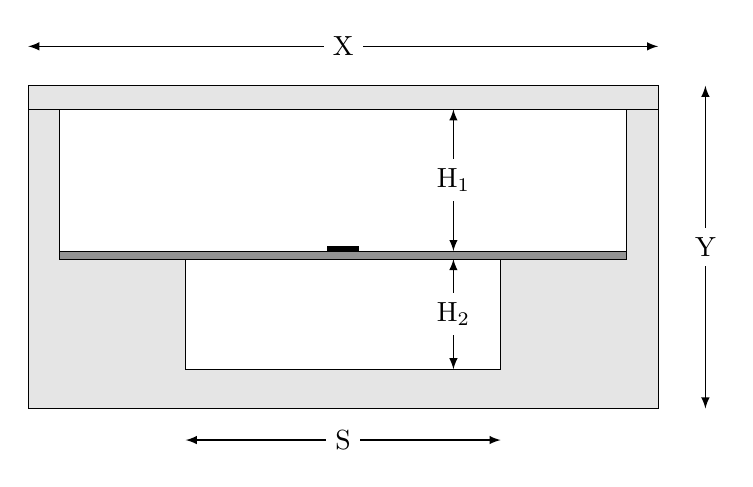
\begin{tikzpicture}[scale=0.2]
		% Case
		\draw[fill=gray!20] plot coordinates
			{(0,0) (0,-19) (40,-19) (40,0) (38,0) (38,-9.508) (30,-9.508) (30,-16.508) (10,-16.508) (10,-9.508) (2,-9.508) (2,0) (0,0)};
		% PCB
		\draw[fill=gray!85] plot coordinates  {(2,-9.508) (2,-9) (38,-9) (38,-9.508) (2,-9.508)};
		% Trace
		\draw[fill=black] plot coordinates {(19,-9) (21,-9) (21,-8.7) (19, -8.7) (19,-9)};
		% Lid
		\draw[fill=gray!20] plot coordinates {(0,0) (0,1.5) (40,1.5) (40,0) (0,0)};
		% Body Dimensions
		\draw[latex-latex] (0,4) -- (40, 4) node[midway,fill=white]{X};
		\draw[latex-latex] (43,1.5) -- (43, -19) node[midway,fill=white]{Y};
		% SS Dimensions
		\draw[latex-latex] (27,-9.508) -- (27, -16.508) node[midway,fill=white]{$\text{H}_2$};
		\draw[latex-latex] (27,0) -- (27, -9) node[midway,fill=white]{$\text{H}_1$};
		\draw[latex-latex] (10,-21) -- (30, -21) node[midway,fill=white]{S};
	\end{tikzpicture}
	\caption[Cross-section of the suspended stripline with critical dimensions]{Cross-section of the suspended stripline with critical dimensions. X=\num{33}, Y=\num{20}, S=\num{20}, $\text{H}_1$=\num{9.5}, $\text{H}_2$=\num{7}, all values in \si{\mm}.}
	\label{fig:cross_section}
\end{figure}

We drew the stripline geometry in ANSYS's 2D Extractor, and solved for the RLGC parameters as a function of frequency from \qtyrange{0.1}{3}{\GHz} in \num{51} uniform steps and as a function of trace width from \qtyrange{0.05}{15}{\mm} swept logarithmically with \num{111} steps per decade.

Next, we designed the section of the amplifier following the input matching network in Keysight's Advanced Design System (ADS).
We used models of lumped components from Modelithics and the Diramics-provided model of the first stage transistor.
This section of the design was unremarkable and used standard techniques.
We used resistive matching to achieve wideband, high output return loss.
We accomplished interstage matching with a single series capacitor.
We designed the second stage active bias following the vendor's recommendation.
Once we completed this design, we created a layout to perform a full wave EM co-simulation with the component circuit models, a crucial step in solving layout-related stability issues.
Finally, we exported the partial amplifier S and noise parameters for the final optimization step of this work.
The schematic for the amplifier is shown in \autoref{fig:schematic}.

\begin{figure}[t]
	\centering
	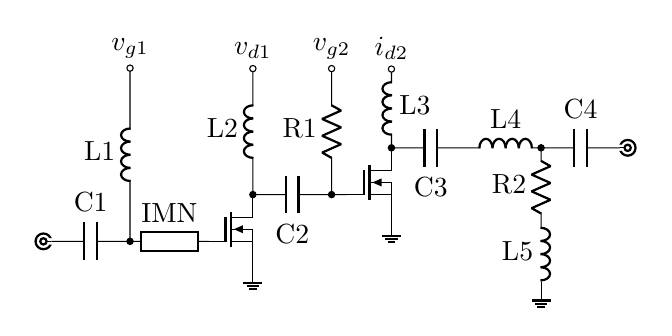
\begin{tikzpicture}
		\ctikzset{nodes width/.initial=0.1}
		\ctikzset{bipoles/length=0.8cm}
		\ctikzset{nodes width/.initial=.05}

		\draw (0,0) node[bnc](In){} to[C=C1, -*] ++(1,0) coordinate (Gin)
		(Gin) to[L=L1] ++(0,2.2) to[short,-o] ++(0,0) node[above]{$v_{g1}$}
		(Gin) to[mstline, mstlinelen=0.9, l=IMN] ++(1,0) coordinate (Q1G)
		(Q1G) -- ++(0,0) node[nigfetd, anchor=G](Q1){}
		(Q1.S) -- ++(0,0) node[ground]{}
		(Q1.D) -- ++(0.0,0) node[short]{} coordinate (Q1D)
		(Q1D) to[L=L2, *-] ++(0,1.6) to[short,-o] ++(0,0) node[above]{$v_{d1}$}
		(Q1D) to[C, l_=C2] ++(1,0) coordinate (Vg2)
		(Vg2) to[R=R1, *-] ++(0,1.6) to[short,-o] ++(0,0) node[above]{$v_{g2}$}
		(Vg2) -- ++(0.2,0) node[nigfetd, anchor=G](Q2){}
		(Q2.S) -- ++(0,0) node[ground]{}
		(Q2.D) -- ++(0.0,0) node[short]{} coordinate (Q2D)
		(Q2D) to[L,l_=L3, *-] ++(0,1) to[short,-o] ++(0,0) node[above]{$i_{d2}$}
		(Q2D) to[C,l_=C3] ++(1,0) to[L=L4] ++(0.9,0) coordinate (out_match)
		(out_match) to[R,l_=R2,*-] ++(0,-1) to[L, l_=L5] ++(0,-0.7) to ++(0,0) node[ground]{}
		(out_match) to[C=C4] ++(1,0) node[bnc, rotate=-180](Out){} ;
	\end{tikzpicture}
	\caption[Schematic of the RF-portion of the LNA]{Schematic of the RF-portion of the amplifier. C1=3x\qty{47}{\pF}, C2=\qty{2.5}{\pF}, C3=\qty{2}{\pF}, C4=\qty{20}{\pF}, L1=\qty{100}{\nH}, L2,L3=\qty{120}{\nH}, L4=\qty{2}{\nH}, L5=\qty{4.7}{\nH}, R1=5.1k$\Omega$, R2=41.2$\Omega$} %fixme hack for JMW
	\label{fig:schematic}
\end{figure}

\begin{figure}[t]
	\centering
	\begin{tikzpicture}
		\begin{axis}[ymin=-10,
        ymax=10,
        unit vector ratio*=1 1,
        width=13cm,
        xlabel=X (\si{\mm})
        ylabel=Y (\si{\mm})]
			\addplot [name path=upper,draw=none] table[x expr=\thisrow{x}*1000,y expr=\thisrow{y}/2*1000, col sep=comma] {shape.csv};
			\addplot [name path=lower,draw=none] table[x expr=\thisrow{x}*1000,y expr=-\thisrow{y}/2*1000, col sep=comma] {shape.csv};
			\addplot [fill=black] fill between[of=upper and lower];
		\end{axis}
	\end{tikzpicture}
	\caption{Optimized NTL input matching network}
	\label{fig:shape}
\end{figure}

We wrote the NTL optimization code in the Julia programming language~\cite{bezansonJuliaFreshApproach2017a}, an open-source, high-level, high-performance language for scientific computing.
This language has an extensive ecosystem in both AD and in nonlinear optimization.
Further, the AD implementations in Julia typically outperform implementations in other languages.

In Julia, we collected the RLGC data from the 2D EM simulation, as well as the S and noise parameters from the circuit simulation.
We used the RLGC data to create a linear interpolation across width and frequency for each parameter.
We constructed the optimization problem with \textit{Optimization.jl}.
This package exposes a structure for defining arbitrary, constrained optimization problems that provide their gradients using a pluggable AD backend.
We used the state-of-the-art package \textit{Enzyme.jl}~\cite{mosesInsteadRewritingForeign2020} as the reverse-mode AD backend as-is with no modifications.
We limited the optimization domain to widths between \qty{0.1}{\mm} and \qty{15}{\mm} and lengths between \qty{50}{\mm} and \qty{120}{\mm}.
We set the constraints such that the input return loss was greater than \qty{\sim9}{\dB} for every point in frequency, representing a compromise between match and noise.

We solved the optimization problem for \num{100} sections, with an initial profile of a \qty{100}{\mm}-length linear taper from \qty{15}{\mm} to \qty{0.1}{\mm} using the \textit{Ipopt} solver~\cite{wachterImplementationInteriorpointFilter2006}.
On an Intel Xeon Gold 6128 workstation, \num{50} iterations were completed in under \qty{5}{\s}.
As gradient-based optimization only finds a local minimum, we ran the optimizer from different starting vectors to compare a few different results.
The problem was robust against initial conditions, as solving with different starting profiles resulted in similar line shapes of equal performance.
% This aligns with the conclusion from~\cite{miazgaDiscreteShapeOptimization2008}, where discrete shape optimization ``seems to be convex''.
In the worst initial case of random widths, the solver took around 2x longer to converge.
However, we know a priori the transformer should transition from \qty{50}{\ohm} to the high $Z_\text{Opt}$, so a linear profile is a reasonable initial condition.
The resulting shape is shown in \autoref{fig:shape}.

Finally, we simulated the resulting geometry in a full-wave 3D EM solver to validate performance.
Following this simulation, we removed a section of the line to place low-loss DC-blocking capacitors and added a high-$Z$ stub for the DC gate bias.
This geometry was added at the lowest-$Z$ section of the NTL to minimize the perturbation.
We re-simulated the geometry to verify the performance with the DC block and bias structures.

To compare the presented AD method to a commercial EDA tool, we constructed the equivalent optimization problem in ADS, using the same interpolated RLGC data.
To prevent ADS from re-simulating the circuit following the NTL, we optimized against the exported S and noise parameters.
The timing results are shown in \autoref{tbl:opt_compare} for various finite-difference (FD) and gradient-free (GF) methods.
All trials achieved the same noise temperature within \qty{0.1}{\K}, with the AD approach around 40x faster than the next best solver in ADS.

\begin{table}[h!]
    \caption{Runtime Comparison of NTL Optimization Methods}
    \label{tbl:opt_compare}
    \label{table_example}
    \centering
    \begin{tabular}{c c c}
         Solver & Runtime (s) &  Relative Time \\
         \hline& \\[-2.0ex]
         \textbf{Ipopt (Reverse-Mode AD)} & \textbf{5} & \textbf{1.0} \\
         Gradient Descent (FD) & 193 & 38.6 \\
         Quasi-Newton (FD) & 1718 & 343.6 \\
         Simulated Annealing (GF) & 3026 & 605.2  \\
         Genetic (GF) & 25200 & 5040.0 \\
    \end{tabular}
\end{table}

\begin{figure}[t!]
	\centering
	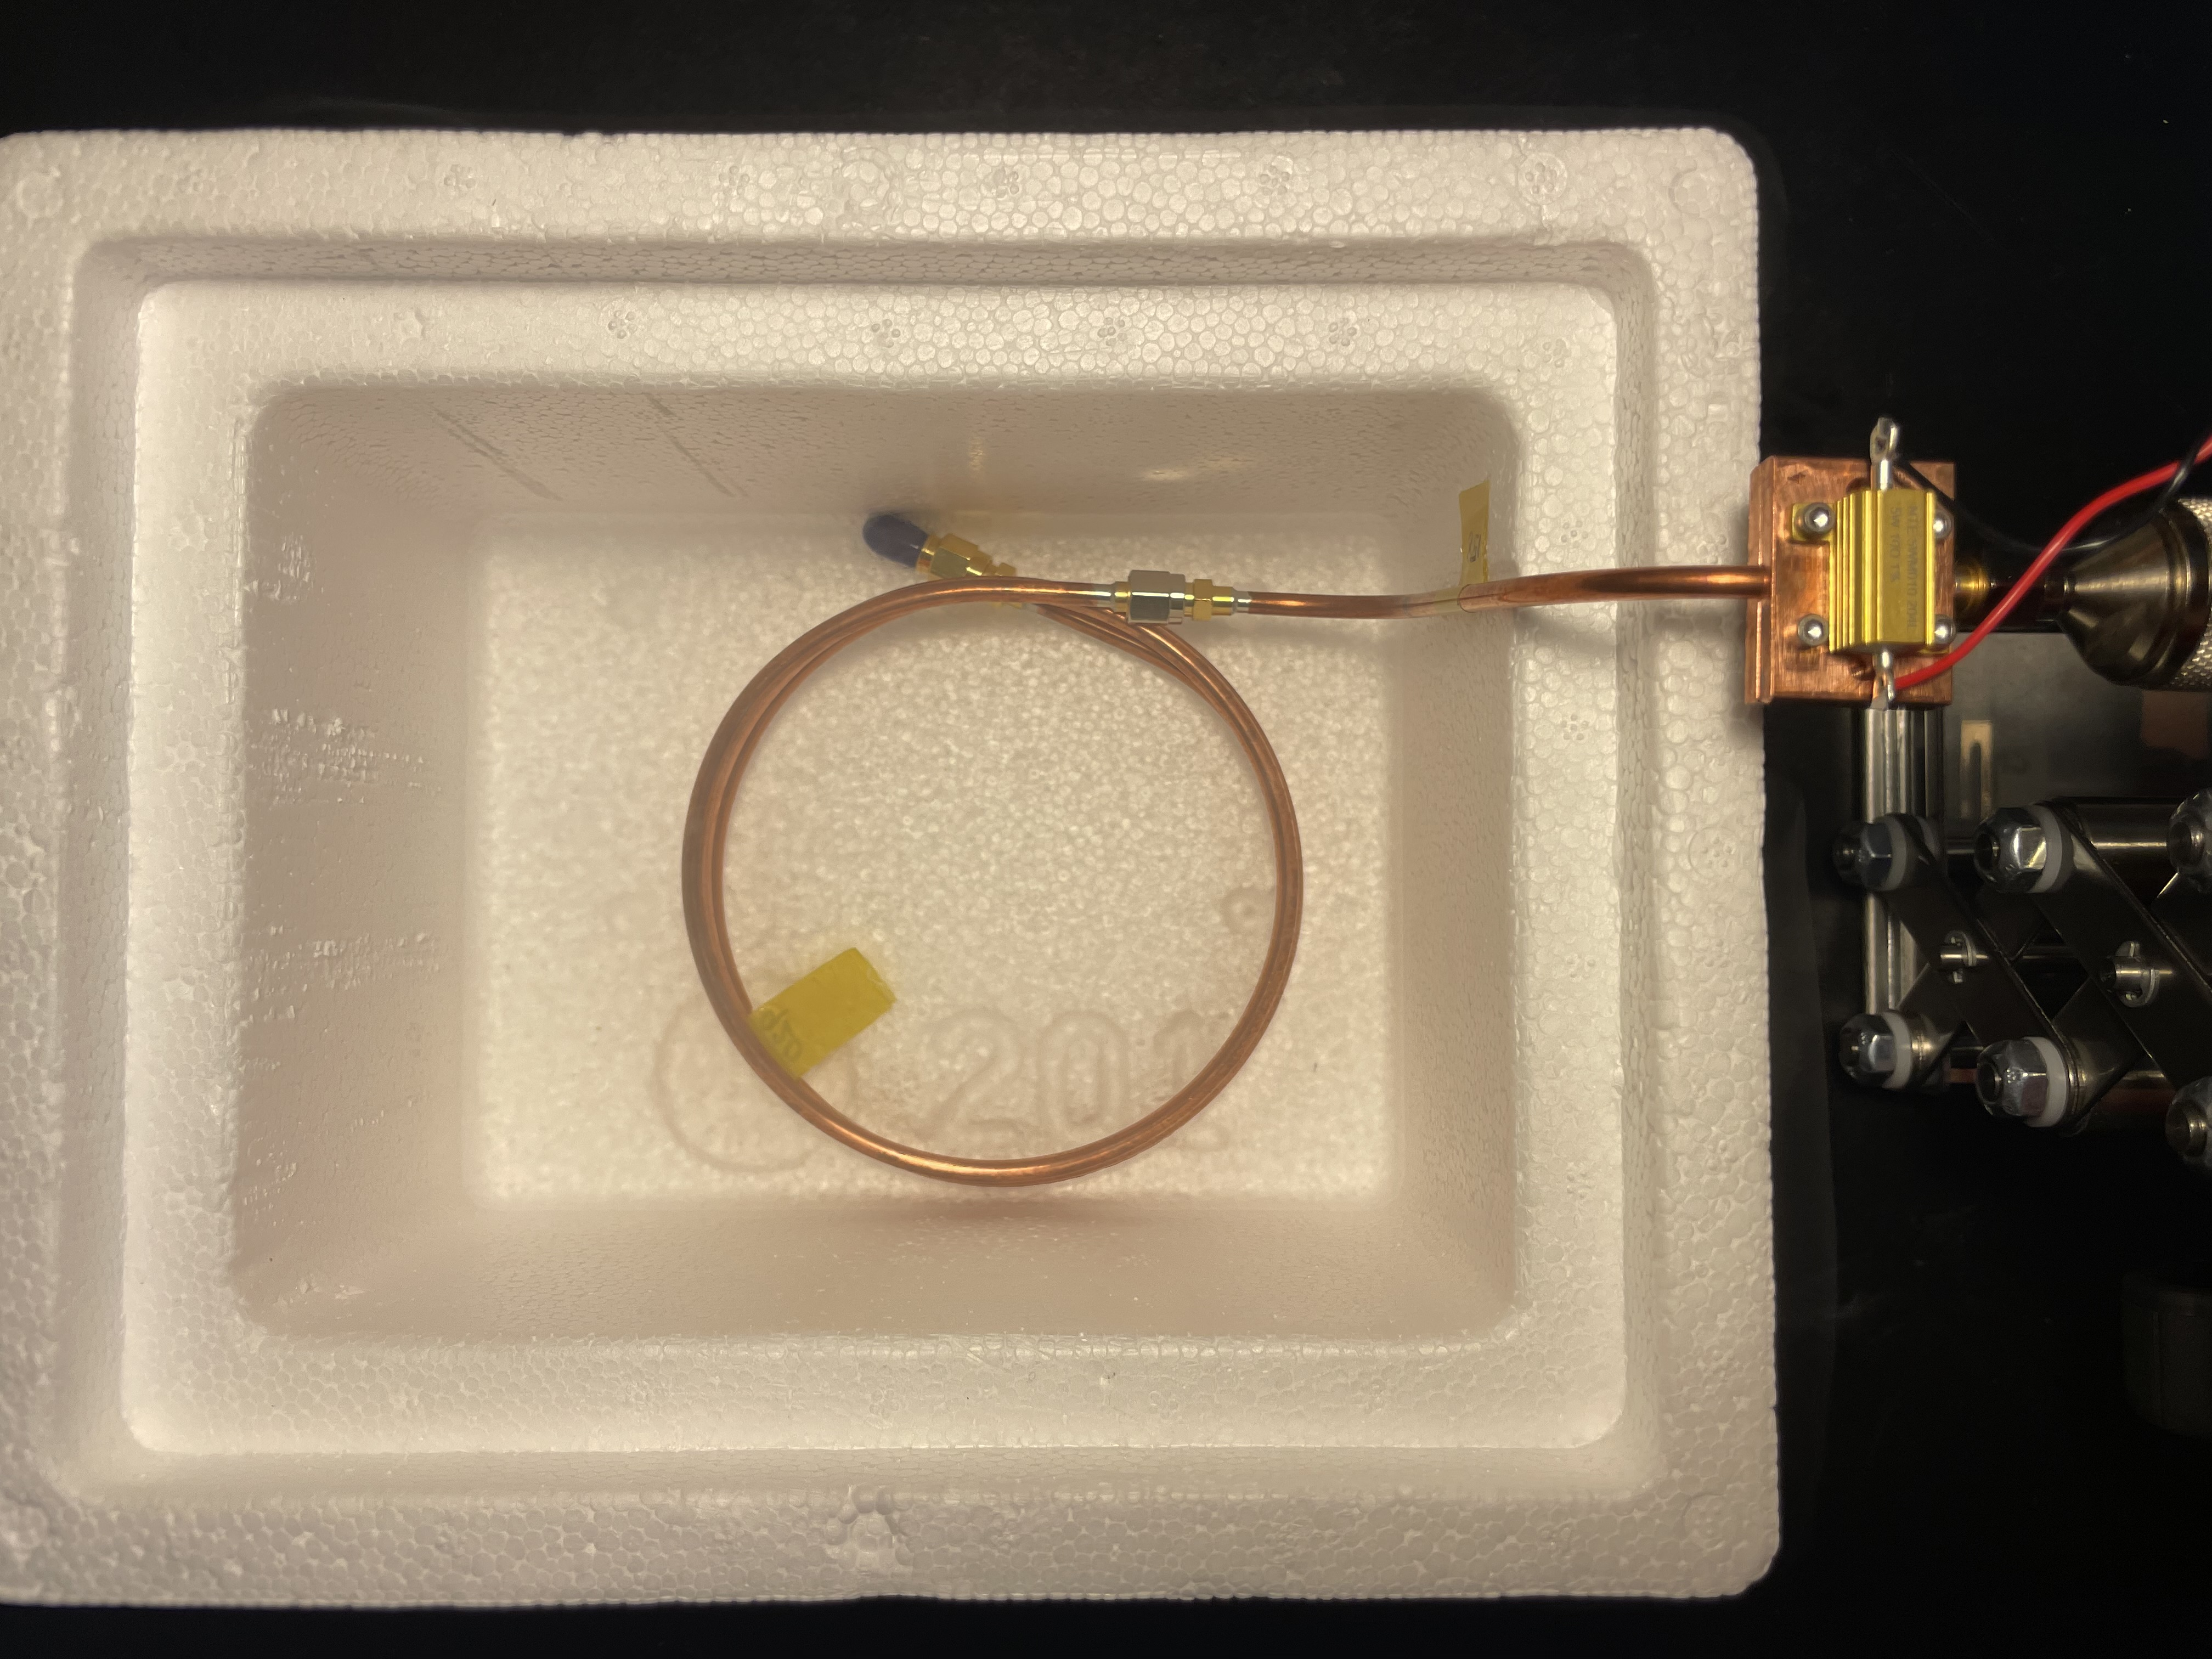
\includegraphics[width=0.75\linewidth]{figures/cold_Load.jpg}
	\caption{\LN{} cold termination measurement setup}
	\label{fig:cold_load}
\end{figure}

\section{Experimental Results} \label{sec:measurement}
\subsection{Noise Measurement Procedure}

Since the amplifier in this work is incredibly low noise, we measured the noise using the Y-factor method with a termination in liquid nitrogen (\LN{}) and a separate room-temperature termination.
If we know the atmospheric pressure, then we precisely know the boiling point of \LN{}.
Then, given the temperature of the cold termination, we need to consider the length of coax that exits the \LN{} bath, its frequency-dependent insertion loss, and its temperature gradient.
As the thermal conductivity of most materials is dependent on their temperature, the temperature gradient along the length of the coax line is nonlinear and must be solved numerically, as described in~\cite{solimanThermalModellingCoaxial2016}.

Next, we must consider the thermal load on the cold termination.
Even when submerged, heat from the warm side of the line will travel into the termination.
To reduce this effect, we could use a stainless steel line, as it has low thermal conductivity.
However, the temperature-dependent conductivity (and therefore insertion loss) of stainless steel is not well known.
Instead, we follow the submerged termination with a long length of line before exiting the bath.
In our case, we used an \qty{8}{\cm} section of RG402 coax connected to a submerged \qty{1}{\m} coil and termination.
We used a heater, shown in \autoref{fig:cold_load}, to maintain the warm end of the coax at ambient temperature.
Finally, we attached a previously characterized N to SMA adapter to the warm end of the cold load to mate with the N-type socket on the constructed LNA.
This setup, shown in \autoref{fig:cold_load}, has a frequency-dependent output noise following this curve-fit result:
%
\begin{equation}
	T_{\text{Cold}}\,\text{(K)} = 78.0824 + 1.2425f_{\si{\GHz}} -  0.1166f_{\si{\GHz}}^{2}
	\label{eqn:tcold}
\end{equation}
%
The error on this result depends on uncertainty in the length of the coax between the surface of the \LN{} and the heater (nominally \qty{8}{\cm}), the warm-side temperature (nominally \qty{297}{\K}), and the atmospheric pressure (nominally \qty{100}{\kilo\Pa}).
Assuming worst-case errors of \qty{\pm 1}{\cm} of length, \qty{\pm 2}{\C} in temperature, and \qty{\pm 0.5}{\kilo\Pa} of pressure, we derive an error model in frequency:
%
\begin{equation}
	\delta T_{\text{Cold}}\,\text{(K)} = 0.0776 + 0.0568f_{\si{\GHz}} - 0.0048f_{\si{\GHz}}^{2}
	\label{eqn:terr}
\end{equation}

\begin{figure}[t]
	\centering
	\begin{circuitikz}[european]
		\ctikzset{nodes width/.initial=0.1}
		\ctikzset{bipoles/length=0.8cm}
		\ctikzset{nodes width/.initial=.05}

		\draw
		(0,0) node[plain mono amp, font=\footnotesize] (dut) {DUT}
		(1.3,0) node[plain mono amp, font=\footnotesize] (rx_amp) {PA}
		(2.1,0) node[msport,circuitikz/RF/scale=2, font=\footnotesize](ADC) {RX}
		(dut.in) to[short] ++(-1.7,0) to[R,l_={$T_{H,C}$}] ++(0,-1) node[tlground]{}
		(dut.out) -- (rx_amp.in)
		(rx_amp.out) -- (ADC) ;

		%\draw[->]  (dut.in) ++(0,0.75) -- (2.1,0.75) node[midway,yshift=1em] {$G$};

		\draw [->, >=Stealth] (-1,-0.5) node[below]{$\Gamma_{\text{A}}$} |- (-0.7,-.1) ;
		\draw [->, >=Stealth] (-1.7,-0.5) node[below]{$\Gamma_{\text{S}_{H,C}}$} |- (-2.0,-.1);
		\draw [->, >=Stealth] (-1,0.5) node[above]{$T_A$} |- (-0.7,.1);

	\end{circuitikz}
	\caption[System schematic of the Y-factor measurement]{System schematic of the Y-factor measurement. The device under test (DUT) is presented a termination with reflection coefficients $\Gamma_{\text{S}_H}$ and $\Gamma_{\text{S}_C}$ at two temperatures $T_H$ and $T_C$, respectively. The DUT is followed by a series of preamplifiers (PA) before being digitized by the receiver (RX). The total noise temperature referred to the input of the DUT is $T_A$. The reflection coefficient at the input of the device under test is $\Gamma_\text{A}$}
	\label{fig:yfac_schematic}
\end{figure}

Finally, we must consider the errors due to changing source impedance between the hot and cold states.
These errors are present in all Y-factor measurements but are exacerbated in our \LN{} approach as there are two distinct terminations.
The impact on the measured Y-factor stems from two effects: the shift in the amplifier's effective input noise due to its noise parameters \eqref{eq:noise} and changes in available gain.

First, to use the Y-factor method, we must assume that the amplifier's noise remains constant between the two states, implying that the impact of the noise parameters is negligible.
Given that we measured both terminations to have return loss \qty{>=25}{\dB} and simulated $R_n$ \qty{<=2}{\ohm} and $|\Gamma_{\text{Opt}}|$ \num{<=0.6}, we expect no worse than \qty{0.03}{\K} error due to this assumption.

Next, we evaluate the impact due to changes in available gain.
Given a termination at the input of a noisy receiver, shown in \autoref{fig:yfac_schematic}, the output noise is given by
%
\begin{equation}
	P = k_{b}BD_\text{RX}G_\text{A}\left(T_{H,C}+T_\text{A}\right)
	\label{eq:noise_power}
\end{equation}
%
where $k_b$ is Boltzmann's constant, $B$ is the noise equivalent bandwidth, $D_\text{RX}$ is a scaling term capturing other digital and analog gain factors in the receiver, $T_{H,C}$ is the hot or cold noise temperature at the amplifier input, $T_\text{A}=T_\text{A}(\Gamma_{\text{S}_{H,C}})$ is the equivalent input noise temperature, and $G_\text{A} = G_\text{A}(\Gamma_{\text{S}_{H,C}})$ is the available gain of the amplifier given by
%
\begin{equation}
	G_{\text{A}} = \frac
	{|S_{21}|^{2}\left(1 - |\Gamma_{S}|^{2}\right)}
	{|1-\Gamma_{S}\Gamma_A|^{2} \left(1-|S_{22}|^2\right)}
\end{equation}
%
We write our expression for the measured Y-factor as a ratio of these hot and cold powers \cite{hpnoise1983}, but now without the assumption that $G_\text{A}$ remains constant due to the impact of $\Gamma_{\text{S}_{H,C}}$:
%
\begin{equation}
	Y =
	\frac
	{P_\text{H}}
	{P_\text{C}} =
	\frac
	{G_{\text{A,H}}\left(T_\text{H} + T_\text{A}\right)}
	{G_{\text{A,C}}\left(T_\text{C} + T_\text{A}\right)} =
	C\left(
	\frac
	{T_\text{H} + T_\text{A}}
	{T_\text{C} + T_\text{A}}
	\right)
	\label{eq:y_fac}
\end{equation}
%
where the correction $C$ due to mismatch error~\cite{heymannGuideNoiseMicrowave2021} is
%
\begin{equation}
	C =
	%\left(
	\frac
	{1 - |\Gamma_{S_\text{H}}|^{2}}
	{1 - |\Gamma_{S_\text{C}}|^{2}}
	%\right)
	%\left(
	\frac
	{|1-\Gamma_{S_\text{C}}\Gamma_A|^{2}}
	{|1-\Gamma_{S_\text{H}}\Gamma_A|^{2}}
	%\right)
\end{equation}
%
Solving \eqref{eq:y_fac} for $T_\text{A}$ yields:
%
\begin{equation}
	T_\text{A} = \frac{T_{\text{H}}-T_{\text{C}}Y/C}{Y/C-1}
	\label{eqn:corrected_yfac}
\end{equation}
%
This equation for noise temperature is identical to the standard expression, but with a correction term applied to Y.
Usually, this factor is close to unity, but as our amplifier is primarily designed for noise and not return loss, and the noise is exceptionally low, the interaction between $\GA$ and $\Gamma_\text{S}$ results in a nontrivial correction.
For our amplifier and terminations, $C$ is between \num{0.974} and \num{1.019}, representing a change in the computed noise of about \qtyrange{2}{4}{\K}, or a third of the total expected noise.

\begin{figure}[t]
	\centering
	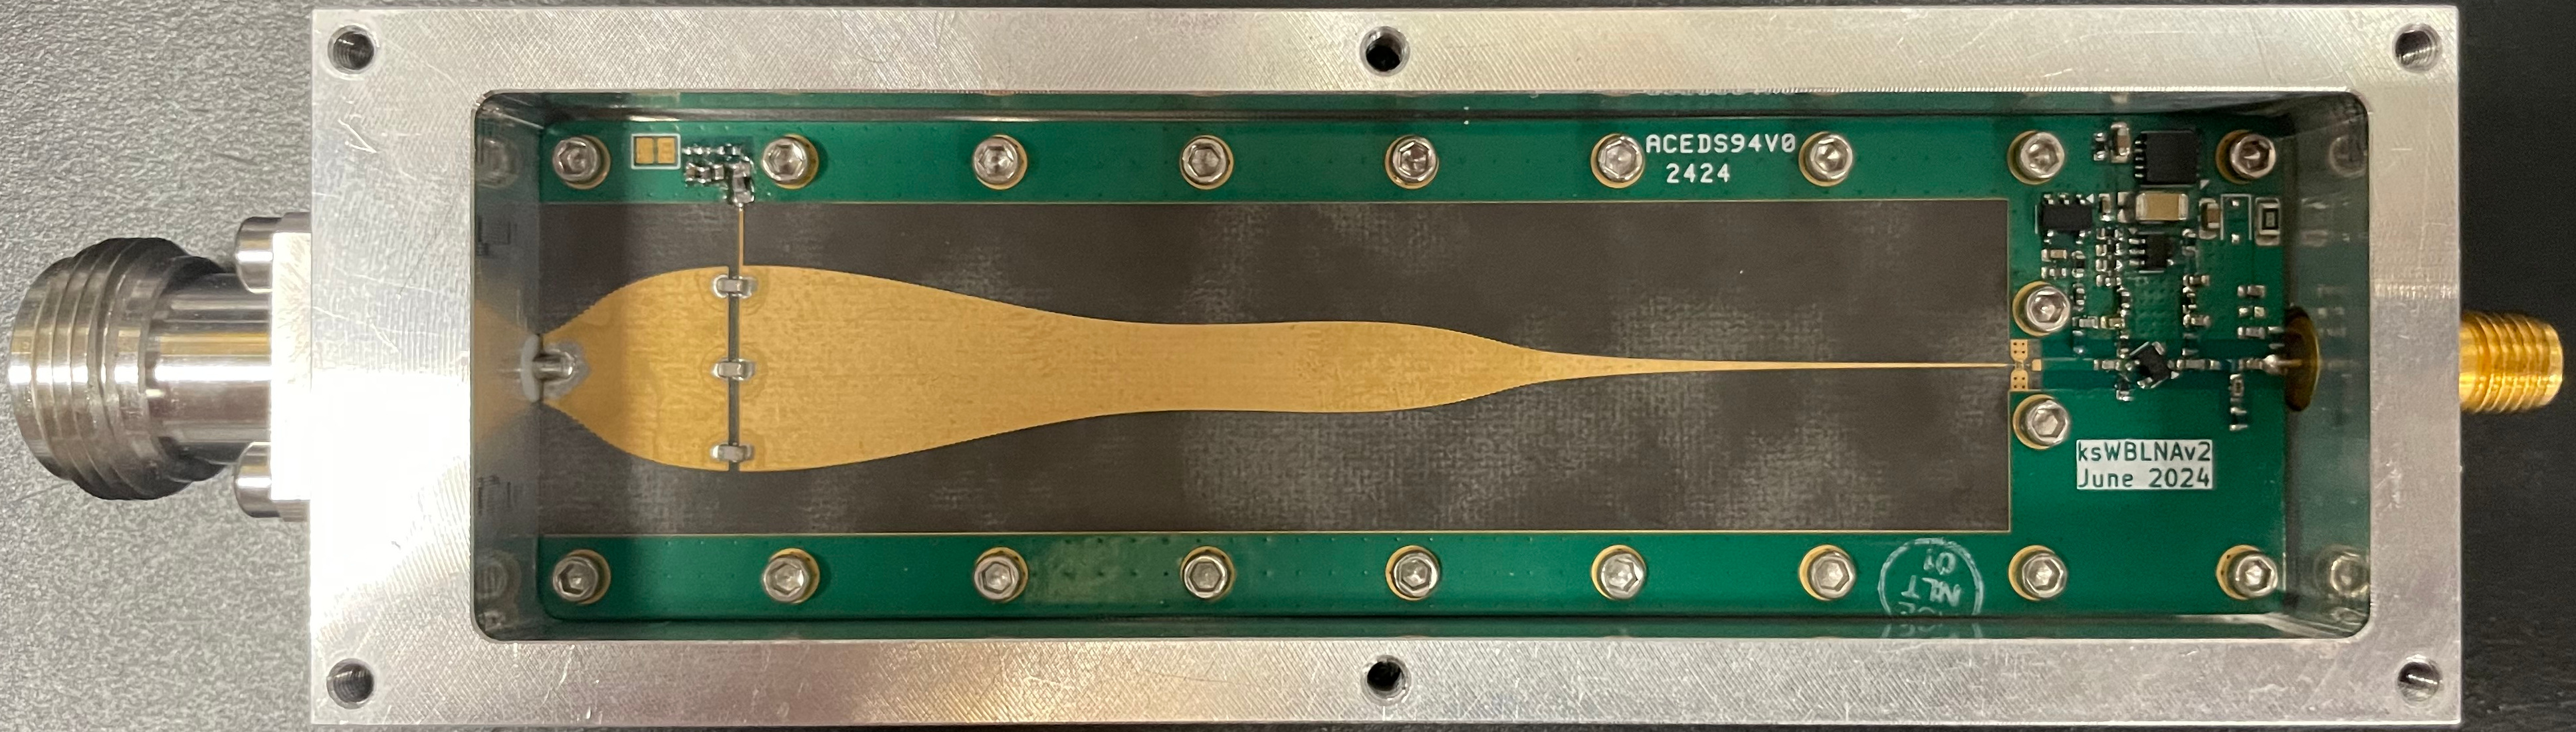
\includegraphics[width=\linewidth]{figures/LNA.jpg}
	\caption{The assembled amplifier in a machined aluminum enclosure with terminations and the lid removed}
	\label{fig:LNA}
\end{figure}

Additionally, we have uncertainty in the reflection coefficient measurements, which results in uncertainty in this correction factor.
Following the datasheet for our network analyzer~\cite{Keysight2Port4Port2018}, we create a curve-fit function to describe the uncertainty in both phase and magnitude, as a function of magnitude.
For our frequency range and IF bandwidth, these are:
\begin{equation}
	\delta|\Gamma| = 0.004 + 0.006|\Gamma|\left(1+|\Gamma|\right)
\end{equation}
and
\begin{equation}
	\delta\arg(\Gamma) = \frac{0.25^{\circ}}{|\Gamma|} + 0.5^{\circ}
\end{equation}

Finally, we need to remove the noise of the receiver.
We do so by performing a measurement with a room temperature termination on the receiver's input and subtracting the linear power from the hot and cold powers of the device under test.
We performed all these calculations also in the Julia language, making use of the \textit{Measurements.jl}~\cite{giordanoUncertaintyPropagationFunctionally2016} package to propagate uncertainty.

\clearpage
\begin{figure}[ht!]
	\centering
    
	\begin{tikzpicture}
		\begin{axis}[
				xlabel={Frequency (\si{\GHz})},
				ylabel={\si{\dB}},
				ymin=-40,ymax=0,
                xmin=0.7,xmax=2.1,
				width=13cm,
				height=6cm,
                xtick={},ytick={},
                minor tick num=1,
                grid=both,
                grid style={line width=.1pt, draw=gray!10},
                major grid style={line width=.2pt,draw=gray!50},
			]
			% S11
			\addplot[mark=none, very thick] table [x expr=\thisrow{freq}/1e9, y=s11, col sep=comma] {meas_s.csv};
			\addplot[mark=none, dashed, very thick] table [x expr=\thisrow{freq}/1e9, y=s11, col sep=comma] {sim_s.csv};
			% S22
			\addplot[mark=none, red, very thick] table [x expr=\thisrow{freq}/1e9, y=s22, col sep=comma] {meas_s.csv};
			\addplot[mark=none, red, dashed, very thick] table [x expr=\thisrow{freq}/1e9, y=s22, col sep=comma] {sim_s.csv};
            % Annotations
            \node[black, font=\footnotesize] at (axis cs: 1.15,-3) {$S_{11}$};
            \node[red, font=\footnotesize] at (axis cs: 1,-30) {$S_{22}$};
		\end{axis}
	\end{tikzpicture}
	\caption{Measured (solid) versus simulated (dashed) S parameters}
	\label{fig:s_compare_11_22}

    \begin{tikzpicture}
		\begin{axis}[
				xlabel={Frequency (\si{\GHz})},
				ylabel={\si{\dB}},
				ymin=34,ymax=40,
                xmin=0.7,xmax=2.1,
				width=13cm,
				height=6cm,
                xtick={},ytick={},
                minor tick num=1,
                grid=both,
                grid style={line width=.1pt, draw=gray!10},
                major grid style={line width=.2pt,draw=gray!50},
			]
            % S21
			\addplot[mark=none, black, very thick] table [x expr=\thisrow{freq}/1e9, y=s21, col sep=comma] {meas_s.csv};
			\addplot[mark=none, black, dashed, very thick] table [x expr=\thisrow{freq}/1e9, y=s21, col sep=comma] {sim_s.csv};
		\end{axis}
	\end{tikzpicture}
    \caption{Measured (solid) versus simulated (dashed) $S_{21}$}
    \label{fig:s_compare_21}

	\begin{tikzpicture}
		\begin{axis}[
				xlabel={Frequency (\si{\GHz})},
				ylabel={Noise Temperature (\si{\K})},
				ymin=8,ymax=17,
				xmin=0.7,xmax=2.1,
				width=13cm,
				height=6cm,
                xtick={},ytick={},
                minor tick num=1,
                grid=both,
                grid style={line width=.1pt, draw=gray!10},
                major grid style={line width=.2pt,draw=gray!50},
			]

			% KS LNA
			\addplot[mark=none, very thick] table [x=f, y=t, col sep=comma] {NTL.csv};
			\addplot [name path=upper,draw=none] table[x=f,y expr=\thisrow{t}+\thisrow{e}, col sep=comma] {NTL.csv};
			\addplot [name path=lower,draw=none] table[x=f,y expr=\thisrow{t}-\thisrow{e}, col sep=comma] {NTL.csv};
			\addplot [fill=black!10] fill between[of=upper and lower];

			% Simluated result
			\addplot[mark=none, dashed, very thick] table [x expr=\thisrow{freq} / 1e9, y=t, col sep=comma] {sim_data.csv};

			% SW LNA
			\addplot[mark=none, red, very thick] table [x=f, y=t, col sep=comma] {2-Step.csv};
			\addplot [name path=upper,draw=none] table[x=f,y expr=\thisrow{t}+\thisrow{e}, col sep=comma] {2-Step.csv};
			\addplot [name path=lower,draw=none] table[x=f,y expr=\thisrow{t}-\thisrow{e}, col sep=comma] {2-Step.csv};
			\addplot [fill=red!10] fill between[of=upper and lower];
		\end{axis}
	\end{tikzpicture}

	\caption{Measured (solid) and simulated (dashed) noise temperature of this work (lower trace), prior work~\cite{shiRoomTemperatureLowNoiseAmplifier2023} (higher trace), and 95\% confidence regions}
	\label{fig:noise_compare}
\end{figure}
\newpage
\subsection{Measured Results}

We measured the S parameters of the assembled amplifier (shown in \autoref{fig:LNA}) and the hot and cold terminations with a Keysight N5242A network analyzer with no averaging or smoothing.
We used a Siglent SSA3032X as the noise receiver, preceded by a Mini-Circuits ZX60-P105LN+ amplifier and bias tee.
We configured the spectrum analyzer to measure from \qtyrange{0.6}{2.1}{\GHz} with a resolution bandwidth of \qty{1}{\MHz}, video bandwidth of \qty{1}{\kHz}, attenuation of \qty{0}{\dB}, preamplifier enabled, and log power averaging.
After a \qty{30}{\minute} warm-up time, data were saved for the noise of the receiver and the device under test with the hot and cold terminations, recording the physical temperatures.
All measurements were performed at an ambient temperature of \qty{297}{\K}.
We performed these power measurements five times each, saving the batch mean and standard deviation.
In error analysis, we used these standard deviation data divided by $\sqrt{5}$ as the standard error of measurement.

We processed the measurements by computing the corrected Y-factor from \eqref{eqn:corrected_yfac}, including uncertainty.
Finally, these data were smoothed with a \qty{150}{\MHz} sliding window.
The results are shown in \autoref{fig:noise_compare}.
The average noise temperature from \qtyrange{0.7}{2}{\GHz} is \newnoise{}.
The measured S parameters match the simulation well, as shown in \autoref{fig:s_compare_11_22} and \autoref{fig:s_compare_21}, with disagreement in $S_{22}$ due to an un-modeled output connector interface.
$S_{21}$ is reasonably flat with \qty{>=35}{\dB} across the band and has a maximum of \qty{39}{\dB}, and $S_{11}$ is \qty{<=-8}{\dB}.
Differences between the simulated and measured $S_{11}$ and $S_{21}$ are due to imperfect wire bond geometry.

We performed these measurements on the amplifier from the prior work~\cite{shiRoomTemperatureLowNoiseAmplifier2023} using the same test setup, procedure, and physical temperature to ensure a fair comparison.
The results of this new measurement are also shown in \autoref{fig:noise_compare}.
Our measurements of the average noise temperature for the prior amplifier is \oldnoise.
Comparing the two amplifiers across the same frequencies, the presented design shows a \improvement mean improvement.
As shown in \autoref{tbl:amp_compare}, the presented amplifier outperforms not only the prior work in noise, but also other similar uncooled amplifiers intended for radio astronomy over a wide bandwidth.

\section{Conclusion}
In this chapter, we demonstrated the design of a non-uniform transmission line LNA input matching network using AD-accelerated gradient-based optimization.
This amplifier achieves a frequency-averaged noise temperature of \newnoise from \qtyrange{0.7}{2}{\GHz} at \qty{297}{\K}.
The NTL design outperforms a previous uniform-line design by \improvement.
This design method is algorithmically more efficient than finite-difference optimization, and outperforms such solvers by more than \num{40}x for this problem.
AD is a general-purpose method for computing derivates and could be adopted for many other microwave problems such as parameter estimation and sensitivity analysis, as well as inverse design of structures besides NTLs.

\begin{table}[h!]
    \centering
    \begin{threeparttable}
    \caption{Comparison of Similar Radio Astronomy LNAs}
    \label{tbl:amp_compare}
        \begin{tabular}{c c c c c}
             Ref. & Freq. (GHz) & $S_{21}$ (dB) & $T_{50}$\tnote{1} (K) &  Topo. / Tech. \\
             \hline& \\[-2.0ex]
             \textbf{This Work} & 0.7-2 & 36 & \num{11.5 \pm 0.4} & NTL / InP \\
             \cite{shiRoomTemperatureLowNoiseAmplifier2023} & 0.7-2 & 40 & \num{12.5 \pm 0.4}\tnote{2} & UTL / InP \\
            \cite{lai0315GHzLNAWideband2023} & 0.3-1.5 & 32 & \num{18 \pm 6} & Discrete / InP \\
            \cite{belostotskiSub02DBNoise2007} & 0.7-1.4 & 17 & 20 & CMOS \\
        \end{tabular}
        \begin{tablenotes}
            \item [1] Band-averaged noise temperature with a \qty{50}{\ohm} source impedance
            \item [2] Our measurements of this amplifier
        \end{tablenotes}
    \end{threeparttable}
\end{table}
\printbibliography[heading=subbibliography]
\end{refsection}

\chapter{Analog Signal Path Design for DSA-2000} \label{ch:asp}
\begin{refsection}
The Analog Signal Path (ASP) subsystem in the DSA-2000 is responsible for all the signal processing before digitization.
There is no frequency conversion, so the entire signal path consists of amplifiers, filters, attenuators, and most notably an RF over fiber optic (RFoF) link.
While RFoF links are widely used in radio astronomy~\cite{periniRadioFrequencyFiber2022,menaRadioFrequencyoverFiberLinkLargearray2013,montebugnoliLargeAntennaArray2005}, none have been deployed at the scale of DSA-2000.
This chapter discusses the ASP system as a whole, focusing on the design, implementation, and testing of the RFoF link.
We also describe modifications to the LNA to improve the match to the feed and tests of an LNA with thermoelectric cooling of the first stage transistor, all to further improve the noise.

\section{RF Over Fiber Link}

\begin{figure}[ht!]
    \centering
    \includestandalone[mode=buildnew]{figures/rfof_diagram}
    \caption{RFoF system diagram}
    \label{fig:rfof_diagram}
\end{figure}

To transport the RF signal from each antenna to the processing facility, we are using RF over fiber (RFoF) links.
These links use RF power to directly modulate the current of a solid-state diode laser, resulting in intensity modulated light.
After traveling through up to \qty{20}{\km} of single mode fiber, this optical signal is presented to a photodiode, where it is converted back into RF current.
This style of analog RF transmission is used in cable television and commercial/military antenna remoting applications.
It is important to note that direct modulation is similar, but architecturally very different from digital modulation, where 1s and 0s are achieved by pulsing the laser nearing 100\% modulation depth.
In RF or analog modulation, we operate in the small signal regime of the laser/photodiode transfer function and are subject to their gain, noise, and linearity characteristics.
While this is a simple and inexpensive solution for long-haul analog transmission, the dynamic range is limited by the distortion in the laser and noise from the laser or photodiode, depending on the amount of optical loss in the link.

\subsubsection{Noise}

\begin{figure}[ht!]
    \centering
    \includestandalone[mode=buildnew]{figures/rfof_circuit}
    \caption{RFoF equivalent noise circuit}
    \label{fig:rfof_noise}
\end{figure}

We begin by focusing on the noise figure of the intrinsic laser to photodiode link.
Noise figure is defined as the degradation in signal-to-noise ratio (SNR) from input to output.
The noise at the input is taken as thermal noise in the generator impedance at a reference temperature of $T_0$.
There are several mechanisms by which the SNR is reduced in the link.
There is added thermal noise due to various resistive components, relative intensity noise or RIN in the laser, optical loss in the fiber (whose noise figure is identical to that of a passive RF attenuator~\cite{coxRelationshipGainNoise1996}), and shot noise in the receiving photodiode.
In the simple, direct-modulated diode link we are studying, RIN and shot noise are the dominant terms, and as such we will ignore the various other sources of thermal noise~\cite{coxLimitsPerformanceRFoverfiber2006}.

The relative intensity noise of the laser (RIN) is the mean deviation in optical output power about the mean square output, given by
\begin{equation}
    \text{RIN}~(\text{dB/Hz}) = \frac{\overline{p_L^2}}{P^2} \,.
\end{equation}
RIN is driven by fluctuations in the photon count in the laser gain cavity through various mechanisms.
If the laser were biased well past its threshold current, RIN is dominated by shot noise.
In this regime $\overline{p_L^2}\propto P$, so $\text{RIN}\propto1/P$.
At lower optical power, RIN is dominated by spontaneous emission~\cite{haugTheoryNoiseSemiconductor1967} and is $\propto 1/P^3$.
Unfortunately, this spectrum is not white, unlike pure shot noise.
Near the laser's relaxation resonance, RIN is amplified~\cite{huiChapter1Fundamentals2023}, giving a slope to the power spectral density.
Other device-dependent effects can also strongly shape the spectral and bias-dependent effects.
As the behavior of RIN is strongly laser-dependent, we start with an experiment measuring our laser's RIN.

To measure the laser RIN, we employ the ``subtraction method''~\cite{kashevskyMethodsMeasuringRelative2023}.
This method sidesteps the need for an optical spectrum analyzer by measuring the induced photocurrent noise due to the laser's intensity noise on an RF spectrum analyzer.
This experiment requires two measurements, one with the laser off and one with the laser on.
In the off state (with the photodiode biased), we measure the power spectral density of the receiver with the dark current of the photodiode.
Then, with the laser biased, we repeat the measurement, this time reading a power spectral density of the aforementioned noise sources superimposed with the laser's noise.
With the laser biased, we note the DC photocurrent of the photodiode.
A figure of the test setup is shown in \autoref{fig:rin_test_setup}.

\begin{figure}[ht!]
    \centering
    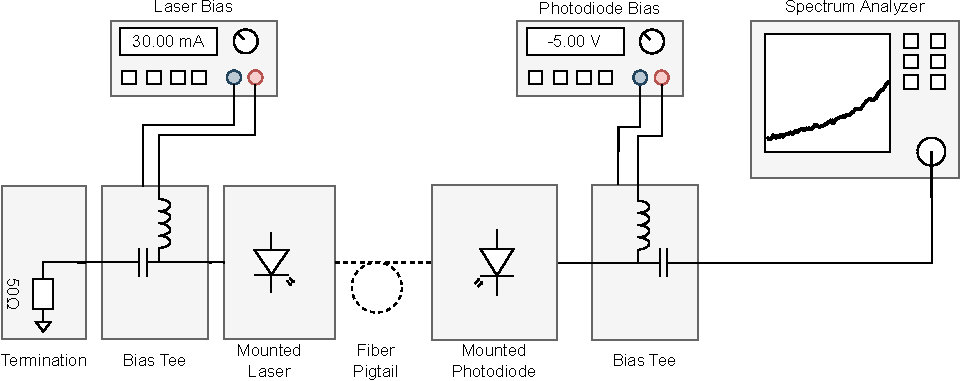
\includegraphics[width=\textwidth]{figures/rin_test.pdf}
    \caption{Diagram of RIN test setup}
    \label{fig:rin_test_setup}
\end{figure}

To compute the link noise alone, we subtract the ``dark'' noise from the measurement with the laser on.
Then, we compute the noise power into the spectrum analyzer from the photodiode's DC shot noise, and subtract that as well to result in just the laser's noise power.
Finally, as the noise power is proportional to $\overline{p_L^2}$, we divide by DC photocurrent's equivalent power to compute RIN, given by
\begin{equation}
    \text{RIN}~(\text{dB/Hz}) = 10\log10{\frac{S_T - S_{RX}-2qI_{PD}Z_0}{I_{PD}^2Z_0}} \,,
\end{equation}
where $S_T$ is the total power spectral density, $S_{RX}$ is the measured ``dark'' power spectral density, $I_{PD}$ is the DC photocurrent, $q$ is the electron charge, and $Z_0$ is the input impedance of the spectrum analyzer.
We then repeat this measurement as a function of bias.
The result of this experiment is shown in \autoref{fig:rin}.
The ripple in this measurement is due to the mismatch between the high impedance photodiode and the length of transmission line and bias tee before the \qty{50}{\ohm} spectrum analyzer input.
Missing data are due to the sensitivity limitations of the spectrum analyzer.

\begin{figure}[ht!]
    \centering
    \includestandalone[mode=buildnew]{figures/rin}
    \caption[Measured RIN of an AGx laser]{Measured RIN of an AGx laser. Top to bottom: \qty{10}{\mA} to \qty{50}{\mA} in steps of \qty{4}{\mA}}
    \label{fig:rin}
\end{figure}

To validate our assumptions about RIN, we look at the bias (optical power) response at several frequencies.
To observe the dependence on laser power instead of laser bias current, however, we need to transform the laser current to power via the laser's threshold current $I_{th}$ and slope efficiency $s$.
As we also have measurements of the DC photocurrent, and know the photodiode's responsivity $\eta$ and an approximate less-than-unity gain (loss) of the connector interface $G_O$, we can estimate the optical power from that direction as well.
From the datasheet, $I_{th}$\qty{=8}{\mA}, $s$\qty{=0.315}{\W/\A}, $\eta$\qty{=0.93}{\A/\W}.
We estimate $G_O$ to be \num{0.98}.

\begin{figure}[ht!]
    \centering
    \includestandalone[mode=buildnew]{figures/laser_pi}
    \caption{Laser output power vs. laser current and DC photocurrent}
    \label{fig:laser_pi}
\end{figure}

Looking at the response in \autoref{fig:laser_pi}, we observe that the datasheet values and our assumptions agree.
This implies we can use either conversion factor to compute laser power instead of disconnecting the laser and attaching it to an optical power meter.

\begin{figure}[ht!]
    \centering
    \includestandalone[mode=buildnew]{figures/rin_v_power}
    \caption{Measured RIN of an AGx laser vs laser output at three frequencies}
    \label{fig:rin_v_power}
\end{figure}

\autoref{fig:rin_v_power} shows the RIN versus laser power at a few frequencies.
We observe the steep increase in RIN at low laser power due to spontaneous emission, and the linear section due to shot noise at higher power, matching our prediction.

To aid in analysis, we ignore the frequency dependence for now and fit a simple quadratic model at \qty{1.5}{\GHz}
\begin{equation}
    \text{RIN}_\text{Model} = -131.2 - 5.5P + 0.19P^2 \,,
    \label{eq:rin_model}
\end{equation}
where $P$ is the laser output power in mW, also plotted in \autoref{fig:rin_v_power}.

Now that we understand the bias and frequency response of RIN, we continue with our noise analysis.
In the small signal case, the laser appears as a small resistor $R_L$, with deviations in current manifesting as deviations in the intensity of the light following the slope efficiency of the laser.
The RIN is then superimposed over this modulated light, creating a mean square deviation over the DC optical power $P$ following
\begin{equation}
    \overline{p_L^2} = \text{RIN}\cdot P^2B \,.
\end{equation}
Finally, the light is attenuated by the less-than-unity gain of the fiber, $G_O$, and is converted back into current following the photodiode's responsivity.
As the laser is biased to a fixed optical output from which it is then modulated, the DC photocurrent generates shot noise in the photodiode following
\begin{equation}
    \overline{i_P^2} = 2qI_PB = 2qPG_O\eta B \,.
\end{equation}
The equivalent noise circuit for this system is shown in \autoref{fig:rfof_noise}.

We simplify this circuit by combining the dependent sources and moving the noise currents forward towards the output, Port 2.
The total current gain between the laser input and the photodiode is
\begin{equation}
    g_i = sG_O\eta \,.
\end{equation}
Noise in the optical power of the laser manifests as noise in the photocurrent, scaled by the square of the passive gain of the fiber and the photodiode responsivity, $(G_O\eta)^2$.
As the shot noise and RIN are uncorrelated, the total noise current is their sum given by
\begin{equation}
    \overline{i_\text{Out}^2} = \overline{p_L^2}(G_O\eta)^2 + \overline{i_P^2} = PG_O\eta B(PG_O\eta\cdot\text{RIN} + 2q) \,.
\end{equation}
The simplified, output-referred circuit is shown in \autoref{fig:rfof_noise_output}.
\begin{figure}[ht!]
    \centering
    \includestandalone[mode=buildnew]{figures/rfof_output_current}
    \caption{RFoF output-referred current noise}
    \label{fig:rfof_noise_output}
\end{figure}

It is usual to work in input-referred noise and here we encounter the first quirk in noise analysis, where instead of simply referring $\overline{i_\text{Out}^2}$ to the input by $g_i^2$, we must consider the impact of the source termination.
Definitionally, noise figure is the degradation in SNR, where the ``signal'' originates from a power source, i.e., with a source impedance.
This is emblematic of the difficulty in this type of analysis, as it would seem that moving the currents forward in the previous case is the same as moving them backwards towards the input.
However, the subtle distinction here is that moving forward is asking, "how does current changing at the input branch manifest as current at the output", which depends solely on the gain, whereas moving backwards is asking, "what equivalent current at the input would manifest as current at the output", which depends on the circuitry attached to the input.
We begin to solve this problem by working backwards, starting with the current we want at the input under the source termination condition and working towards the output.

\begin{figure}[ht!]
    \centering
    \includestandalone[mode=buildnew]{figures/rfof_input_current}
    \caption{RFoF input-referred current noise}
    \label{fig:rfof_noise_input}
\end{figure}

In this configuration, we use the current divider to find
\begin{equation}
    i_L = i_\text{In}\frac{R_S}{R_L+R_S} \,.
\end{equation}
Then, we use the current gain to move to the output
\begin{equation}
    i_\text{Out} = g_ii_\text{In}\frac{R_S}{R_L+R_S} \,.
\end{equation}
Finally, we solve for $i_\text{In}$ in terms of $i_\text{Out}$, and take the time average of the square
\begin{equation}
    \overline{i_\text{In}^2} = \frac{\overline{i_\text{Out}^2}}{g_i^2}\left(\frac{R_L}{R_S}+1\right)^2 \,.
\end{equation}

To find the noise figure, we use the relation
\begin{equation}
    F = \frac{\overline{i_\text{Total}^2}}{\overline{i_S^2}} = \frac{\overline{i_\text{In}^2} + \overline{i_S^2}}{\overline{i_S^2}} = \frac{\overline{i_\text{In}^2}}{\overline{i_S^2}} + 1 \,,
\end{equation}
where $\overline{i_S^2}$ is the thermal noise in the generator, defined as
\begin{equation}
    \overline{i_S^2} = 4k_BT_0G_SB \,,
\end{equation}
where $G_S$ is the source conductance and $T_0$ \qty{=290}{\K} (IEEE standard).
Combining these equations yield
\begin{equation}
    F = 1 + \frac{\overline{i_\text{Out}^2}\left(\frac{R_L}{R_S}+1\right)^2}{4k_BT_0G_SBg_i^2} \,.
\end{equation}
Finally, as we prefer to work in equivalent noise temperature, we use $T_e = T_0(F-1)$, we find
\begin{equation}
    T_e  = \frac{PR_S}{4k_Bs^2G_O\eta}\left(PG_O\eta\cdot\text{RIN} + 2q\right)\left(\frac{R_L}{R_S}+1\right)^2 \,.
    \label{eq:link_noise}
\end{equation}

This equivalent noise temperature result gives insight into the behavior of the link under different source impedances.
If we are free to choose $R_S$ through matching, we would want to know what $R_S$ provides the best noise performance.
We solve for this quantity by minimizing \autoref{eq:link_noise}, finding the $R_S$ that solves $\delta T_e/\delta R_s=0$.
Taking the positive solution of the quadratic yields
\begin{equation}
    R_{S,\text{Opt}} = R_L \,.
\end{equation}
This follows from the fact that all the noise sources are not electrically influenced by the source impedance, so by conjugate matching the laser, we maximize the link's gain and therefore minimize the input-referred noise.
In this case, we can find the minimum noise temperature of
\begin{equation}
    T_\text{Min}  = \frac{PR_L}{k_Bs^2G_O\eta}\left(PG_O\eta\cdot\text{RIN} + 2q\right) \,,
    \label{eq:min_link_noise}
\end{equation}
which is a ratio of
\begin{equation}
    \frac{T_e}{T_\text{Min}} = \frac{(R_S+R_L)^2}{4R_SR_L} \,,
\end{equation}
or \num{3.025} for $R_S$ \qty{=50}{\ohm} and $R_L$ \qty{=5}{\ohm}
The plot for minimum noise alongside the \qty{50}{\ohm} noise is shown in \autoref{fig:link_noise}.
This figure uses typical parameters for our laser\footnote{\url{https://www.agxtech.com/PDF/PLMR3+Rev+4.0.pdf}}, which has a RIN following our model in \autoref{eq:rin_model}, a slope efficiency $s$ of \qty{0.315}{\watt/\ampere}, and a slope impedance of \qty{5}{\ohm} and for our photodiode\footnote{\url{https://www.agxtech.com/PDF/PPDA+R5.6.pdf}}, which has a slope efficiency $\eta$ of \qty{0.93}{\ampere/\watt}.
The conclusion from this plot is that for laser powers between \qty{8}{\mW} and \qty{12}{\mW}, the noise is about the same, within a factor of 2, and remains that way as we increase the loss.

\begin{figure}[ht!]
    \centering
    \includestandalone[mode=buildnew]{figures/link_noise}
    \caption[RFoF link noise]{RFoF link noise ($R_S=$ \qty{50}{\ohm} (solid) and optimal (dotted)) versus optical attenuation}
    \label{fig:link_noise}
\end{figure}

With $T_e(R_S)$ and $R_{S,\text{Opt}}$, we have essentially derived the noise parameters of the RFoF link.
Notably missing from this analysis are the parasitics of the components, the series inductance of the leads of the packaged coaxial laser and photodiode, and the junction capacitance of the photodiode.
To minimize noise, as we have seen, we will want to power match at the input of the network.
As such, any inductance at the input will need to be tuned out in addition to matching the slope resistance.

\subsubsection{S Parameters}

In analyzing the gain and reflection coefficients of the RFoF link, it is more convenient to analyze S parameters instead of voltages and currents.
However, determining the S parameters directly from the \autoref{fig:rfof_noise} model is nontrivial due to the dependent sources.
Instead, it would be easier to consider the Y parameters and convert using the well-known formula.
The Y parameters of \autoref{fig:rfof_noise} are
\begin{equation}
    Y_\text{Link} = \frac{1}{R_L}\begin{bmatrix}
        1 & 0 \\ s\eta G_\text{O} & 0
    \end{bmatrix} \,.
\end{equation}
Converting to S parameters gives
\begin{equation}
    S_\text{Link} = \begin{bmatrix}
        \dfrac{R_L-Z_0}{R_L+Z_0} & 0 \\\\[0.2em] \dfrac{2Z_0s\eta G_\text{O}}{R_L+Z_0} & 1
    \end{bmatrix} \,.
    \label{eq:unmatched_rfof_s}
\end{equation}

$S_{11}$ of this result is as expected, it is simply the reflection coefficient of the laser's slope impedance.
$S_{21}$, however, is more nuanced.
If we substitute numbers into this equation such as $Z_0$=\qty{50}{\ohm}, $R_L$=\qty{5}{\ohm} and $s\eta G_\text{Opt}$=\num{0.2}, we find $|S_{21}|^2$=\qty{-8.79}{dB}.
If we ``match'' the laser by setting the characteristic impedance equal to the laser's impedance $R_L=Z_0$, the equation reduces to $s\eta G_\text{Opt}$.
However, using the same device parameters, we find $|0.2|^2$=\qty{-13.98}{\dB}, unintuitively lower gain than before.
The apparent drop in gain is because the equation for $S_{21}$ assumes both the output and input ports have equivalent characteristic impedance, and changing the output impedance changes the power delivered from the photodiode.
It would be more correct to analyze this circuit with an explicit matching network at the input.

For a real load as we are exploring, we can use an ideal transformer at the input as our matching network, which has an ABCD matrix of
\begin{equation}
    A_{TF} = \begin{bmatrix}
        N & 0\\0 & 1/N
    \end{bmatrix} \,.
\end{equation}
We convert the Y matrix of the link to ABCD parameters using the standard equation to arrive at
\begin{equation}
    A_\text{Link} = -\frac{1}{s\eta G_\text{O}}\begin{bmatrix}
        0 & R_L \\ 0 & 1
    \end{bmatrix} \,.
\end{equation}
We  then cascade to get
\begin{equation}
    A_\text{Combined} = -\frac{1}{s\eta G_\text{O}}\begin{bmatrix}
        0 & NR_L \\ 0 & 1/N
    \end{bmatrix} \,.
\end{equation}
And then finally converting to S parameters, we find
\begin{equation}
    S_\text{Combined} = -\frac{1}{Z_0+N^2R_L} \begin{bmatrix}
        Z_0-N^2R_L & 0 \\ 2NZ_0s\eta G_\text{O} & 1
    \end{bmatrix} \,.
\end{equation}
If $N=\sqrt{Z_0/R_L}$, matching to the laser resistance, this reduces to
\begin{equation}
    S_\text{Matched} = \begin{bmatrix}
        0 & 0 \\ -\sqrt{Z_0}s\eta G_\text{O}/\sqrt{R_L} & 1
    \end{bmatrix} \,.
    \label{eq:matched_rfof_s_params}
\end{equation}
Using the same parameters as before, the matched link now has an $|S_{21}|^2$ of \qty{-3.98}{\dB}, or \qty{4.81}{\dB} higher gain than unmatched.
A notable result from this is that positive power gain can be achieved, even though the intrinsic link exhibits a current gain of less than unity.
For example, if $s\eta G_O$\num{=0.2}, $Z_0$\qty{=50}{\ohm}, and $R_L$\qty{=2}{\ohm}, the link's gain $|S_{21}|$ would be unity.
While unintuitive, the transformer acts as a current gain device, for which a given turns ratio will counteract the current loss in the link.
From both the noise and gain perspective, we want to power match the input of the laser.

\subsection{Linearity}

The final metric we evaluate for the RFoF link is the linearity.
If radio frequency interference (RFI) is strong enough, nonlinearity in the signal chain would result in frequency products in addition to the center frequency of the RFI itself.
The strength of these $n$th-order products depends on the strength of the incoming signal and the $n$th derivative of the transfer function of the system.
One way to reduce the impact of this distortion is to simply limit the incoming signal strength.
Doing so, however, is at odds with added noise, as we want to \textit{increase} power before a noisy component to reduce that component's noise impact on the SNR.
To compare RFoF links (bias settings, laser or photodiode choice, etc.), we use ``spurious free dynamic range'' or (SFDR) as a noise-normalized linearity metric.
SFDR is defined as the maximum signal power at the output for which the power of the $n$-th order intermodulation product is equal to the noise power.
This is defined following~\cite{pozarMicrowaveEngineering2012} as
\begin{equation}
    \text{SFDR}_n~(\text{dB})= \frac{n-1}{n}(\text{OIP}n - N_O) \,,
    \label{eq:sfdr}
\end{equation}
where $\text{OIP}_n$ is the $n$th order output intermodulation intercept point and $N_O$ is the output noise power, both defined in dBm.
We only need to consider $n=3$ for narrowband systems, but our radio telescope is more than an octave, so we must consider second order distortion as well, as distortion products from the lower half of the band will appear in the upper half.

\subsection{Experimental Results}

\subsubsection{Noise}

\begin{figure}[ht!]
    \centering
    \includestandalone[mode=buildnew]{figures/link_noise_in}
    \caption[RFoF link input noise temperature]{RFoF link input noise temperature from \qty{10}{\mA} to \qty{50}{\mA} (top to bottom) in steps of \qty{4}{\mA}}
    \label{fig:link_noise_in}
\end{figure}

To validate our noise derivation, we directly measured the link output noise and referred this to the input.
The setup is identical to that used in the RIN characterization, shown in \autoref{fig:rin_test_setup}.
We used a spectrum analyzer as a power meter to measure the noise power, with the link input terminated with a room-temperature load.
In addition to this ``hot'' measurement, we also measured the noise of the receiver, including the ``dark current'' of the photodiode.
Finally, we subtracted the linear noise powers to leave us with just the noise of the link.
Using measured power gain from a network analyzer, we referred the noise power back to the input.

% For this experiment, we used an AGx \textit{PLMR3-A-1-5-S} laser\urlfootnote{http://www.agxtech.com/PDF/PLMR3+Rev+4.0.pdf}.
% We first measured the slope resistance (or equivalent input impedance) by measuring $S_{11}$ on a network analyzer.
% As the laser was mounted to an SMA connected, we measured an open circuit on a connector of the same length to de-embed the effect of the added electrical length.
% After performing the de-embedding, we find the laser's impedance to be \complexqty{5+25j}{\ohm} at \qty{1.5}{\GHz} and \qty{3.1}{\ohm} near DC.

We measured the noise power spectral density on a spectrum analyzer at the output of the photodiode, subtracting the receiver noise.
The input-referred noise temperature in \autoref{fig:link_noise_in} matches our expected result from \autoref{fig:link_noise}, with high laser currents resulting in an input noise temperature of about \qty{60000}{\K} in the band of interest.
While this is an excellent result, we need to consider both the noise and linearity to compute the SFDR.

\subsubsection{Linearity}

\begin{figure}[ht!]
    \centering
    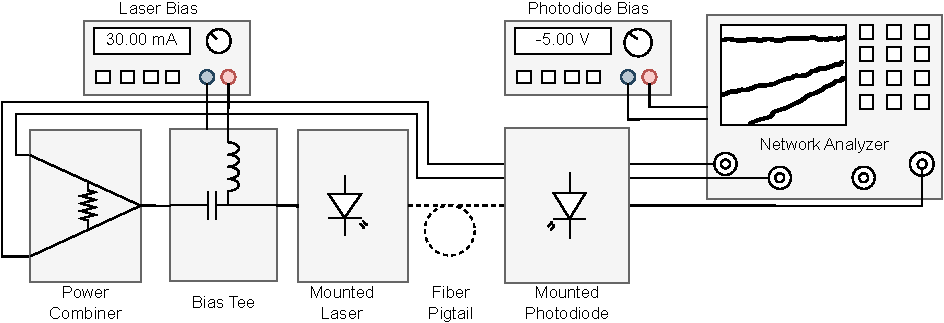
\includegraphics[width=\textwidth]{figures/lin_test.pdf}
    \caption{Diagram of linearity test setup}
    \label{fig:lin_test_setup}
\end{figure}
%
While it is simple to measure noise and gain to validate analytic expressions, linearity is more difficult as we do not have an expression for the actual transfer function of the laser and photodiode pair.
The solution is to probe the individual derivatives of the transfer function by injecting a pair of tones and observing their intermodulation products, derived for reference in \autoref{ch:eqns}.
For the experiment, we inject two closely spaced tones, $\omega_L$ and $\omega_H$ (\qty{1}{\MHz} apart) and observe five tones on the output.
We observe the powers of the two fundamental tones to track the gain, $P_L$ and $P_H$, $\omega_L+\omega_H$ for $\text{IM}_2$ to compute $\text{OIP2}$ via
\begin{equation}
    \text{OIP2}~(\text{dBm}) = P_L+P_H-\text{IM2} \,,
\end{equation}
and $2\omega_H-\omega_L$ for $\text{IM}_{3H}$, and $2\omega_L-\omega_H$ for $\text{IM}_{3L}$ to compute $\text{OIP3}$ via
\begin{align}
    \text{OIP3}~(\text{dBm}) &= \frac{2P_L+P_H-\text{IM3}_{L}}{2}\\
    &= \frac{P_L + 2P_H - \text{IM3}_{H}}{2} \,.
\end{align}
As OIP3 has two unique solutions, we are typically interested in the worst case, which will be the minimum of the two OIP3 results.
For most components, the two terms will be close to equal.
Performing this experiment for the AGx laser and photodiode pair from before, we measured the results shown in \autoref{fig:rfof_oipn}.

\begin{figure}[ht!]%
    \centering
    \subfloat{\includestandalone[mode=buildnew]{figures/laser_oip2}}%
    \quad%
    \subfloat{\includestandalone[mode=buildnew]{figures/laser_oip3}}%
    \caption[RFoF measured OIPn]{RFoF measured OIPn. Red trace is the receiver linearity, black traces bottom to top are laser currents from \qty{10}{\mA} to \qty{50}{\mA} in steps of \qty{2}{\mA}}%
    \label{fig:rfof_oipn}%
\end{figure}

This measurement was performed on a PNA-X network analyzer, utilizing the two independent sources as the two tones incident on the link under test, shown in \autoref{fig:lin_test_setup}.
We used a power combiner to join these two outputs, and calibrated out the loss of the combiner and bias tee to result in an incident power of \qty{-20}{\dBm} for each tone.
The analyzer was then configured to detune the receiver to follow the five tones of interest described earlier, measuring the power directly in dBm.
This measurement includes a correction for the loss in the cable and internals following the photodiode.

Both the IP2 and IP3 results are excellent for this laser, being limited by the dynamic range of the PNA-X in the IP3 measurement.
In the presented range, the gain only changes slightly, from an average of \qty{-5}{\dB} to \qty{-4}{\dB} across the band, with associated input values changing accordingly.
The linearity improves through increased laser power, but then worsens as the device starts to saturate, near \qty{50}{\mA}.

Combining the noise and linearity measurements, we compute the spurious-free dynamic range as defined in \autoref{eq:sfdr}, shown in \autoref{fig:rfof_sfdr}.
%
\begin{figure}[ht!]%
    \centering
    \subfloat{\includestandalone[mode=buildnew]{figures/rfof_sfdr2}}%
    \quad%
    \subfloat{\includestandalone[mode=buildnew]{figures/rfof_sfdr3}}%
    \caption[Spurious-free dynamic range for the intrinsic RFoF link]{Spurious-free dynamic range for the intrinsic RFoF link. Traces bottom to top are laser currents from \qty{10}{\mA} to \qty{50}{\mA} in steps of \qty{2}{\mA}. Noise power is the measured intrinsic link noise under \qty{100}{\kHz} of noise equivalent bandwidth.}%
    \label{fig:rfof_sfdr}%
\end{figure}
%
Here, we see that we are limited primarily by the 2nd-order linearity, although it is important to note that after \qty{1}{\GHz}, the power in the second order tone (\qty{2}{\GHz}) is out of band and will be filtered out).
At high laser powers, in the band of \SIrange{0.7}{2}{\GHz}, we can expect SFDR of better than \qty{60}{\dB} for the intrinsic RFoF link.

As the SFDR falls off at high laser power while the noise improves, we find the optimum laser bias of around \qty{38}{\mA} shown in \autoref{fig:sfdr2_sweep}.

\begin{figure}[ht!]
    \centering
    \includestandalone[mode=buildnew]{figures/sfdr2_sweep}
    \caption{Spurious-free dynamic range for the RFoF link vs laser current}
    \label{fig:sfdr2_sweep}
\end{figure}

\subsection{Long-Haul RFoF}

\begin{figure}[ht!]
    \centering
    \includestandalone[mode=buildnew]{figures/scattering_linearity}
    \caption[Linearity metrics for single- and double- isolated lasers]{Linearity metrics for single- and double- isolated lasers at 0 and \qty{20}{\km}. Both lasers are operated at \qty{40}{mA}.}
    \label{fig:scattering_linearity}
\end{figure}

The final piece of the RFoF puzzle involves the consequences of the exceptionally long fiber that connects the most remote antennas in the telescope to the digitizers.
Current estimates predict the longest fiber lengths will be about \qty{20}{\km}.
As the lasers operate at $1310\,\text{nm}$, the effective loss in standard single-mode fiber is around \qty{0.5}{\dB/\km}.
\autoref{fig:link_noise} indicates that the resulting \qty{10}{\dB} of optical loss (\qty{20}{\dB} in RF power loss) will result in about a factor of four increase in noise.
This is still an acceptable noise level, as there can be a significant amount of gain before the link.

In initial experiments with a \qty{20}{\km} spool on the bench, linearity and noise both worsened significantly more than what was expected.
We believe the origin of these effects are reflections off imperfect connectors and Rayleigh backscattering, coupled with poor isolation in the laser and laser chirp.
While simple reflections are a well-known issue in RFoF links, the induced distortion due to the increased effect of Rayleigh backscattering in long fibers combined with the laser chirp is more nuanced.
Only recently has this effect been discussed in the context of radio astronomy~\cite{periniRadioFrequencyFiber2022,nanniControllingRayleighBackscatteringInducedDistortion2020}.

Rayleigh backscattering is a phenomenon in optical fiber where imperfections in the refractive index results in scattering.
While this would typically manifest as a linear effect (and is the dominant component of loss in fiber optic links~\cite{kanamoriTransmissionLossOptical2021}), the interaction with the chirp of the laser results in nonlinear effects.
Chirp is the change in instantaneous optical frequency of the laser as it is directly modulated.
As Rayleigh backscattering sends a reflected wave back into the laser, the time-dependence of chirp results in the different optical frequencies mixing and retransmitting, resulting in a distorted signal.

There are a few ways one could mitigate the distortion introduced from chirp and scattering.
The most straightforward approach would be to use a lower chirp laser, or to use an external modulator where there would be no chirp.
Both of these solutions, however, are typically expensive.
The solution for one radio telescope (the SKA)~\cite{nanniControllingRayleighBackscatteringInducedDistortion2020} is to introduce a dithering tone.
This low frequency modulation added on top of the RF modulation results in decoherence of the scattered light and the light emitted from the gain cavity of the laser.
This solution, however, requires additional hardware and filtering.
The most simple solution is to instead purchase lasers with more optical isolation built in, or add in-line isolators in the path of the fiber near the laser.
For most vendors, a double isolator (which increases the optical isolation by \qty{20}{\dB}) is on the order of a \$10 increase in cost.

We find that adding additional isolators is an effective way to reduce the nonlinearities introduced by Rayleigh backscattering by repeating the earlier tests on the bench with a \qty{20}{\km} spool\footnote{Thank you, Courtney!}, shown in \autoref{fig:scattering_linearity}.
In this figure, the top row are tests with \qty{0}{\km} of fiber, with the laser and photodiode directly connected.
The bottom row adds a \qty{20}{\km} spool of single-mode fiber between the two.
The left column shows OIP2 and the right column shows OIP3.
All four measurements are shown for the single- and double-isolated lasers.

\begin{figure}[ht!]
    \centering
    \includestandalone[mode=buildnew]{figures/scattering_noise}
    \caption[Noise temperature for single- and double- isolated lasers]{Noise temperature for single- and double- isolated lasers at \qty{0}{\km} (dotted) and \qty{20}{\km} (solid). Both lasers are operated at \qty{40}{mA}}
    \label{fig:scattering_noise}
\end{figure}

From \autoref{fig:scattering_linearity}, it is clear that at \qty{20}{\km} we observe Rayleigh scattering as the linearity for the single-isolated laser is significantly lower.
Adding the double isolator improves the linearity for both second and third order distortion.
It is important to note, however, that the overall output intercept points have dropped in the case of the long fiber.
This is due to the fiber introducing \qty{10}{\dB} of loss, and the primary distortion mechanism is from the laser itself.
If you add the \qty{10}{\dB} of loss back to the \qty{20}{\km} numbers, the double-isolated intercept points match the \qty{0}{\km} measurements, matching our expectations.

We can see similar behavior in noise by measuring the devices in the same manner as described earlier.
The results are shown in \autoref{fig:scattering_noise}\footnote{Ripples are due to uncalibrated cables that connect to the bare diodes, as this measurement was performed on a spectrum analyzer with a tracking generator and not a network analyzer}.
With the single-isolator laser, the noise increases by more than an order of magnitude when we add the \qty{20}{\km} of fiber, which is much more than the predicted results from \autoref{fig:link_noise}.
With the double-isolated laser, however, the noise is almost exactly what we predict of around \qty{2e5}{\K}.

Adding a double isolator is a simple, low-cost solution that significantly improves the performance of the link in the long-haul limit.
Additionally, doing so does not reduce performance in the short-fiber distances.
The output power of the laser is lower in the double-isolated case due to the doubled insertion loss of the isolator, but this only mildly increases the noise.

\section{System Design}

\subsection{Link Budget}

For the DSA-2000, we are presented with a few key science requirements that induce engineering requirements.
For us, the most important metric is survey speed.
Our ability to survey the sky to high sensitivity with a fast cadence is one reason this instrument will be impactful.
Survey speed is a consequence of the radiometer equation, where we compute the RMS uncertainty in a noise measurement by 
\begin{equation}
    \sigma_T = \frac{T_\text{Sys}}{\sqrt{B\tau}} \,,
\end{equation}
given system temperature $T_\text{Sys}$, bandwidth $B$ and integration time $\tau$.
If our goal is to have high confidence in our results, say $5\sigma$ and the telescope has some fixed bandwidth, we have two ``free'' parameters: $T_\text{Sys}$ and $\tau$.
These are free in the sense that $T_\text{Sys}$ is an engineering requirement and $\tau$ is an operational requirement.
If $T_\text{Sys}$ were very low, we could integrate over much less time to achieve the same statistical result.
For a large survey, we must perform this integration for every piece of the sky we want to observe.
As such, driving down $T_\text{Sys}$ is critical for the survey speed performance, quadratically so.

To not significantly perturb the survey speed, we chose to place a limit of no more than \qty{1}{\K} added to $T_\text{Sys}$ from electronics following the LNA.
As the LNA has \qty{\approx35}{\dB} of gain, this implies a maximum tolerable noise of \qty[group-digits = false]{\approx3100}{\K} at the output of the LNA.

Next, we focus on the total gain requirement.
The amount of absolute power required to drive the digitizers is dependent on the exact digitizer we use.
The current design uses the 12-bit AD9207\footnote{\raggedright\url{https://www.analog.com/media/en/technical-documentation/data-sheets/ad9207.pdf}} from Analog Devices.
The full-scale peak-to-peak input voltage is \qty{1.475}{\V} across the differential \qty{100}{\ohm} input.
We want to set the gain of the analog signal path such that the astronomical signal exercises about three bits~\cite{bianchi2008adc}.
A detectable signal must be above the device's quantization noise, reducing the effective bit-depth of the ADC to an ``effective number of bits'' (ENOB).
Our ADC has an ENOB of about 9 at \qty{2}{\GHz}.
This implies that three bits correspond to a peak-to-peak voltage of \qty{23.05}{\mV}, or \qty{-31.78}{\dBm} into the \qty{100}{\ohm} differential input.
At the input of the analog signal path, $T_\text{Sys}$ induces a noise power of \qty{-93.48}{\dBm} (\qty{25}{\K} across our \qty{1.3}{\GHz} bandwidth).
Therefore, we require at least \qty{61.7}{\dB} of gain.
About \qty{35}{\dB} of gain is covered by the LNA, leaving only \qty{26.7}{\dB} needed for the remainder of the ASP.

Finally, we must consider linearity.
The signal levels from astronomical sources will be incredibly faint, so their intermodulation products are unimportant.
Unfortunately, radio frequency interference (RFI) can be terribly strong, wreaking havoc on our science data.
The impact of RFI can be categorized into three domains.
First, if the RFI is faint enough to generate intermodulation products beneath the power of $T_\text{Sys}$, all we must do is flag the carrier channels as contaminated.
Second, the RFI power could be strong enough to generate intermodulation products that also contaminate the science band, implying we would need to flag more than the channel of the RFI.
Finally, the RFI could be so strong that we compress the amplifiers or saturate the ADC, resulting in an unusable signal path.
In the final case, there is not much that can be done in ASP design, depending on what saturates first.
If everything were linear, this gives us \qty{\approx 50}{\dB} of headroom between the ADC noise and the brightest RFI we can tolerate before the ADCs saturate.
This motivates using highly linear amplifiers after the LNA, such that we only need to worry about the ADC.
In the first and second cases, we can derive a constraint in the second and third order intermodulation terms if we want the intermodulation power to be no more than some fraction of the noise power in a channel.

If the signal chain has \qty{61.7}{\dB} of gain and the full-scale power of the ADC is \qty{4.34}{\dBm}, RFI will saturate the ADC at $P_\text{RFI}=$\qty{-57.36}{\dB} into the LNA.
If we constrain the linearity such that the ASP does not generate intermodulation products higher than the noise level of $P_N=$\qty{-93.48}{\dBm} at the input, then we can compute lower limits on the input second-order intercept as $\text{IIP2} = 2P_\text{RFI} - P_N$\qty{=-21.23}{\dBm} and third-order intercept as $\text{IIP3} = (3P_\text{RFI} - P_N)/2$\qty{=-39.29}{\dBm}.
Referred to the output under \qty{61.7}{\dB} of gain, these bounds are an OIP2 and OIP3 of \qty{40.46}{\dBm} and \qty{22.4}{\dBm}, respectively.

\subsection{Cascade Analysis}

To optimize the analog signal path, we compute the input-referred noise and total cascaded linearity.
Computing the total link noise follows from the Friis cascaded noise equation
\begin{equation}
    T_\text{In} = T_\text{LNA} + \frac{T_1}{G_\text{LNA}} + \frac{T_2}{G_\text{LNA}G_2} \dots \,,
\end{equation}
where each subsequent noise contributor is divided by the available gain of all the components before it.
Linearity, however, is again a bit tricky.
As the intermodulation powers are deterministic, they may be in-phase and add coherently.
Following the derivation in~\cite{pozarMicrowaveEngineering2012}, we find the total OIP3 of a cascaded system with coherent products as
\begin{equation}
    \text{OIP3}~(\text{W}) = \left(
    \frac{1}{G_n\text{OIP3}_{{n-1}}} + \frac{1}{\text{OIP3}_{n}}
    \right)^{-1} \,,
\end{equation}
where $G_n$ is the gain of the $n$th component along with its $\text{OIP}_{3_n}$, $\text{OIP}_{3_{n-1}}$ is the cumulative OIP$_3$ through the previous $n-1$ stages.
All of these calculations are performed in linear units.
This equation is a worst-case estimate, assuming every intermodulation product adds coherently.
This will never be the case as there is a relatively random distribution of cable lengths, interconnects, and component phase delays.
As such, we can approximate the phases between each stage to be random, and compute the associated cascaded intercept point as
\begin{equation}
    \text{OIP3}~(\text{W}) = \left(
    \frac{1}{G_n^2\text{OIP3}_{{n-1}}^2} + \frac{1}{\text{OIP3}_{n}^2}
    \right)^{-1/2} \,.
\end{equation}
We can then input-refer these quantities by dividing by the accumulated gain as
\begin{equation}
    \text{IIP}n = \text{OIP}n /G \,.
\end{equation}
Stated another way, if we assume the intermodulation terms have random phase, then their powers would add.
The derivation for 2nd order distortion and cascade analysis can be found in \autoref{ch:eqns}.

Using these results, we compute the cascaded behavior for all the components along the analog signal path, shown in \autoref{tab:casc_asp}.
Our noise only increases by \qty{\approx0.7}{\K}, beneath our requirement of \qty{1}{\K}.
The total gain is \qty{74.7}{\dB}, with adjustable attenuators allowing for control.
We set the attenuators to match our gain requirement and to maximize dynamic range.
Finally, the cascaded OIP2 and OIP3 are \qty{45.83}{\dB} and \qty{33.57}{\dBm} respectively, exceeding our requirements.

\newpage
\begin{landscape}
\begin{table}[!htp]\centering
\caption[Cascade analysis of analog signal path]{Cascade analysis of analog signal path. Included are coherent (Coh.) and random (Rand.) output intercept points. Noise at the input LNA represents the entire system noise temperature. Laser noise is assuming a worst-case of \qty{1e6}{K}. Laser linearity uses the double-isolator result from \autoref{fig:scattering_linearity}. Passive components are taken to have infinite linearity.}\label{tab:casc_asp}
\scriptsize
\begin{tabular}{lr|cccc|ccccccc}\toprule
& &\multicolumn{4}{c}{Component} &\multicolumn{6}{c}{Cascaded} \\\cmidrule{3-12}
Description &Part Number &Gain  &Noise&OIP2 &OIP3 &Acc. Gain &Noise &OIP3 Coh. &OIP3 Rand. &OIP2 Coh. &OIP2 Rand. \\
 & & (dB) & (K) & (dBm) & (dBm) & (dB) & (K) & (dBm) & (dBm) & (dBm) & (dBm) \\\midrule
LNA             & ksWBLNAv2   & 35   & 25     & 22 & 16 & 35   & 25    & 16    & 16    & 22    & 22    \\
Cable           & -           & -3   & 288.63 & -- & -- & 32   & 25.09 & 13    & 13    & 18.99 & 19 \\
Bias Tee        & Lumped      & -0.1 & 6.75   & -- & -- & 31.9 & 25.10 & 12.9  & 12.9  & 18.88 & 18.9 \\
BPF             & Lumped      & -2   & 169.62 & -- & -- & 29.9 & 25.21 & 10.9  & 10.9  & 16.88 & 16.9 \\
Amplifier       & PGA-105     & 15   & 170    & 49 & 39 & 44.9 & 25.38 & 25.69 & 25.89 & 30.75 & 31.82 \\
External Filter & -           & 0    & 0      & -- & -- & 44.9 & 25.38 & 25.69 & 25.89 & 30.72 & 31.82 \\
Attenuator      & F1958       & -2   & 169.62 & 80 & 64 & 42.9 & 25.38 & 23.69 & 23.89 & 28.69 & 29.82 \\
Amplifier       & PGA-105     & 15   & 170    & 49 & 39 & 57.9 & 25.38 & 35.83 & 37.44 & 39.93 & 43.41 \\
Attenuator      & PAT-1220C   & -3   & 288.63 & -- & -- & 54.9 & 25.39 & 32.83 & 34.44 & 36.87 & 40.41 \\
Amplifier       & PGA-105     & 15   & 170    & 49 & 39 & 69.9 & 25.39 & 38.47 & 38.98 & 44.29 & 48.11 \\
BFP             & Lumped      & -1   & 75.09  & -- & -- & 68.9 & 25.39 & 37.47 & 37.98 & 43.17 & 47.1 \\
Attenuator      & PAT-1220C   & -3   & 288.63 & -- & -- & 65.9 & 25.39 & 34.47 & 34.98 & 40.08 & 44.1 \\
Bias Tee        & Lumped      & -0.1 & 6.75   & -- & -- & 65.8 & 25.39 & 34.37 & 34.88 & 39.89 & 44 \\

RFoF Link       & -           & -25  & 1E6    & 20 & 0  & 40.8 & 25.66 & -0.48 & -0.02 & 11.06 & 16.46 \\

Bias Tee        & Lumped      & -0.1 & 6.75   & -- & -- & 40.7 & 25.66 & -0.58 & -0.12 & 10.95 & 16.36 \\
Attenuator      & PAT-1220C   & -3   & 288.63 & -- & -- & 37.7 & 25.68 & -3.58 & -3.12 & 7.95  & 13.36 \\
Amplifier       & PGA-105     & 15   & 170    & 49 & 39 & 52.7 & 25.71 & 11.42 & 11.88 & 22.53 & 28.32 \\
Attenuator      & F1958       & -3   & 288.63 & 80 & 64 & 49.7 & 25.71 & 8.42  & 8.88  & 19.52 & 25.32 \\
BPF             & Lumped      & -1   & 75.09  & -- & -- & 48.7 & 25.71 & 7.42  & 7.88  & 18.51 & 24.32 \\
Amplifier       & PGA-105     & 15   & 170    & 49 & 39 & 63.7 & 25.72 & 22.32 & 22.88 & 32.16 & 38.88 \\
Attenuator      & PAT-1220C   & -3   & 288.63 & -- & -- & 60.7 & 25.72 & 19.32 & 19.88 & 29.14 & 35.88 \\
Amplifier       & PGA-105     & 15   & 170    & 49 & 39 & 75.7 & 25.72 & 33.05 & 34.57 & 40.21 & 46.83 \\
AA Filter       & Distributed & -1  & 75.09   & -- & -- & 74.7 & 25.72 & 32.05 & 33.57 & 39.13 & 45.83 \\
ADC             & AD9207 & & & & & & & & & & \\
\bottomrule
\end{tabular}
\end{table}
\end{landscape}
\newpage

\subsection{FTX and FRX Boards}

\begin{figure}[ht!]%
    \centering
    \subfloat{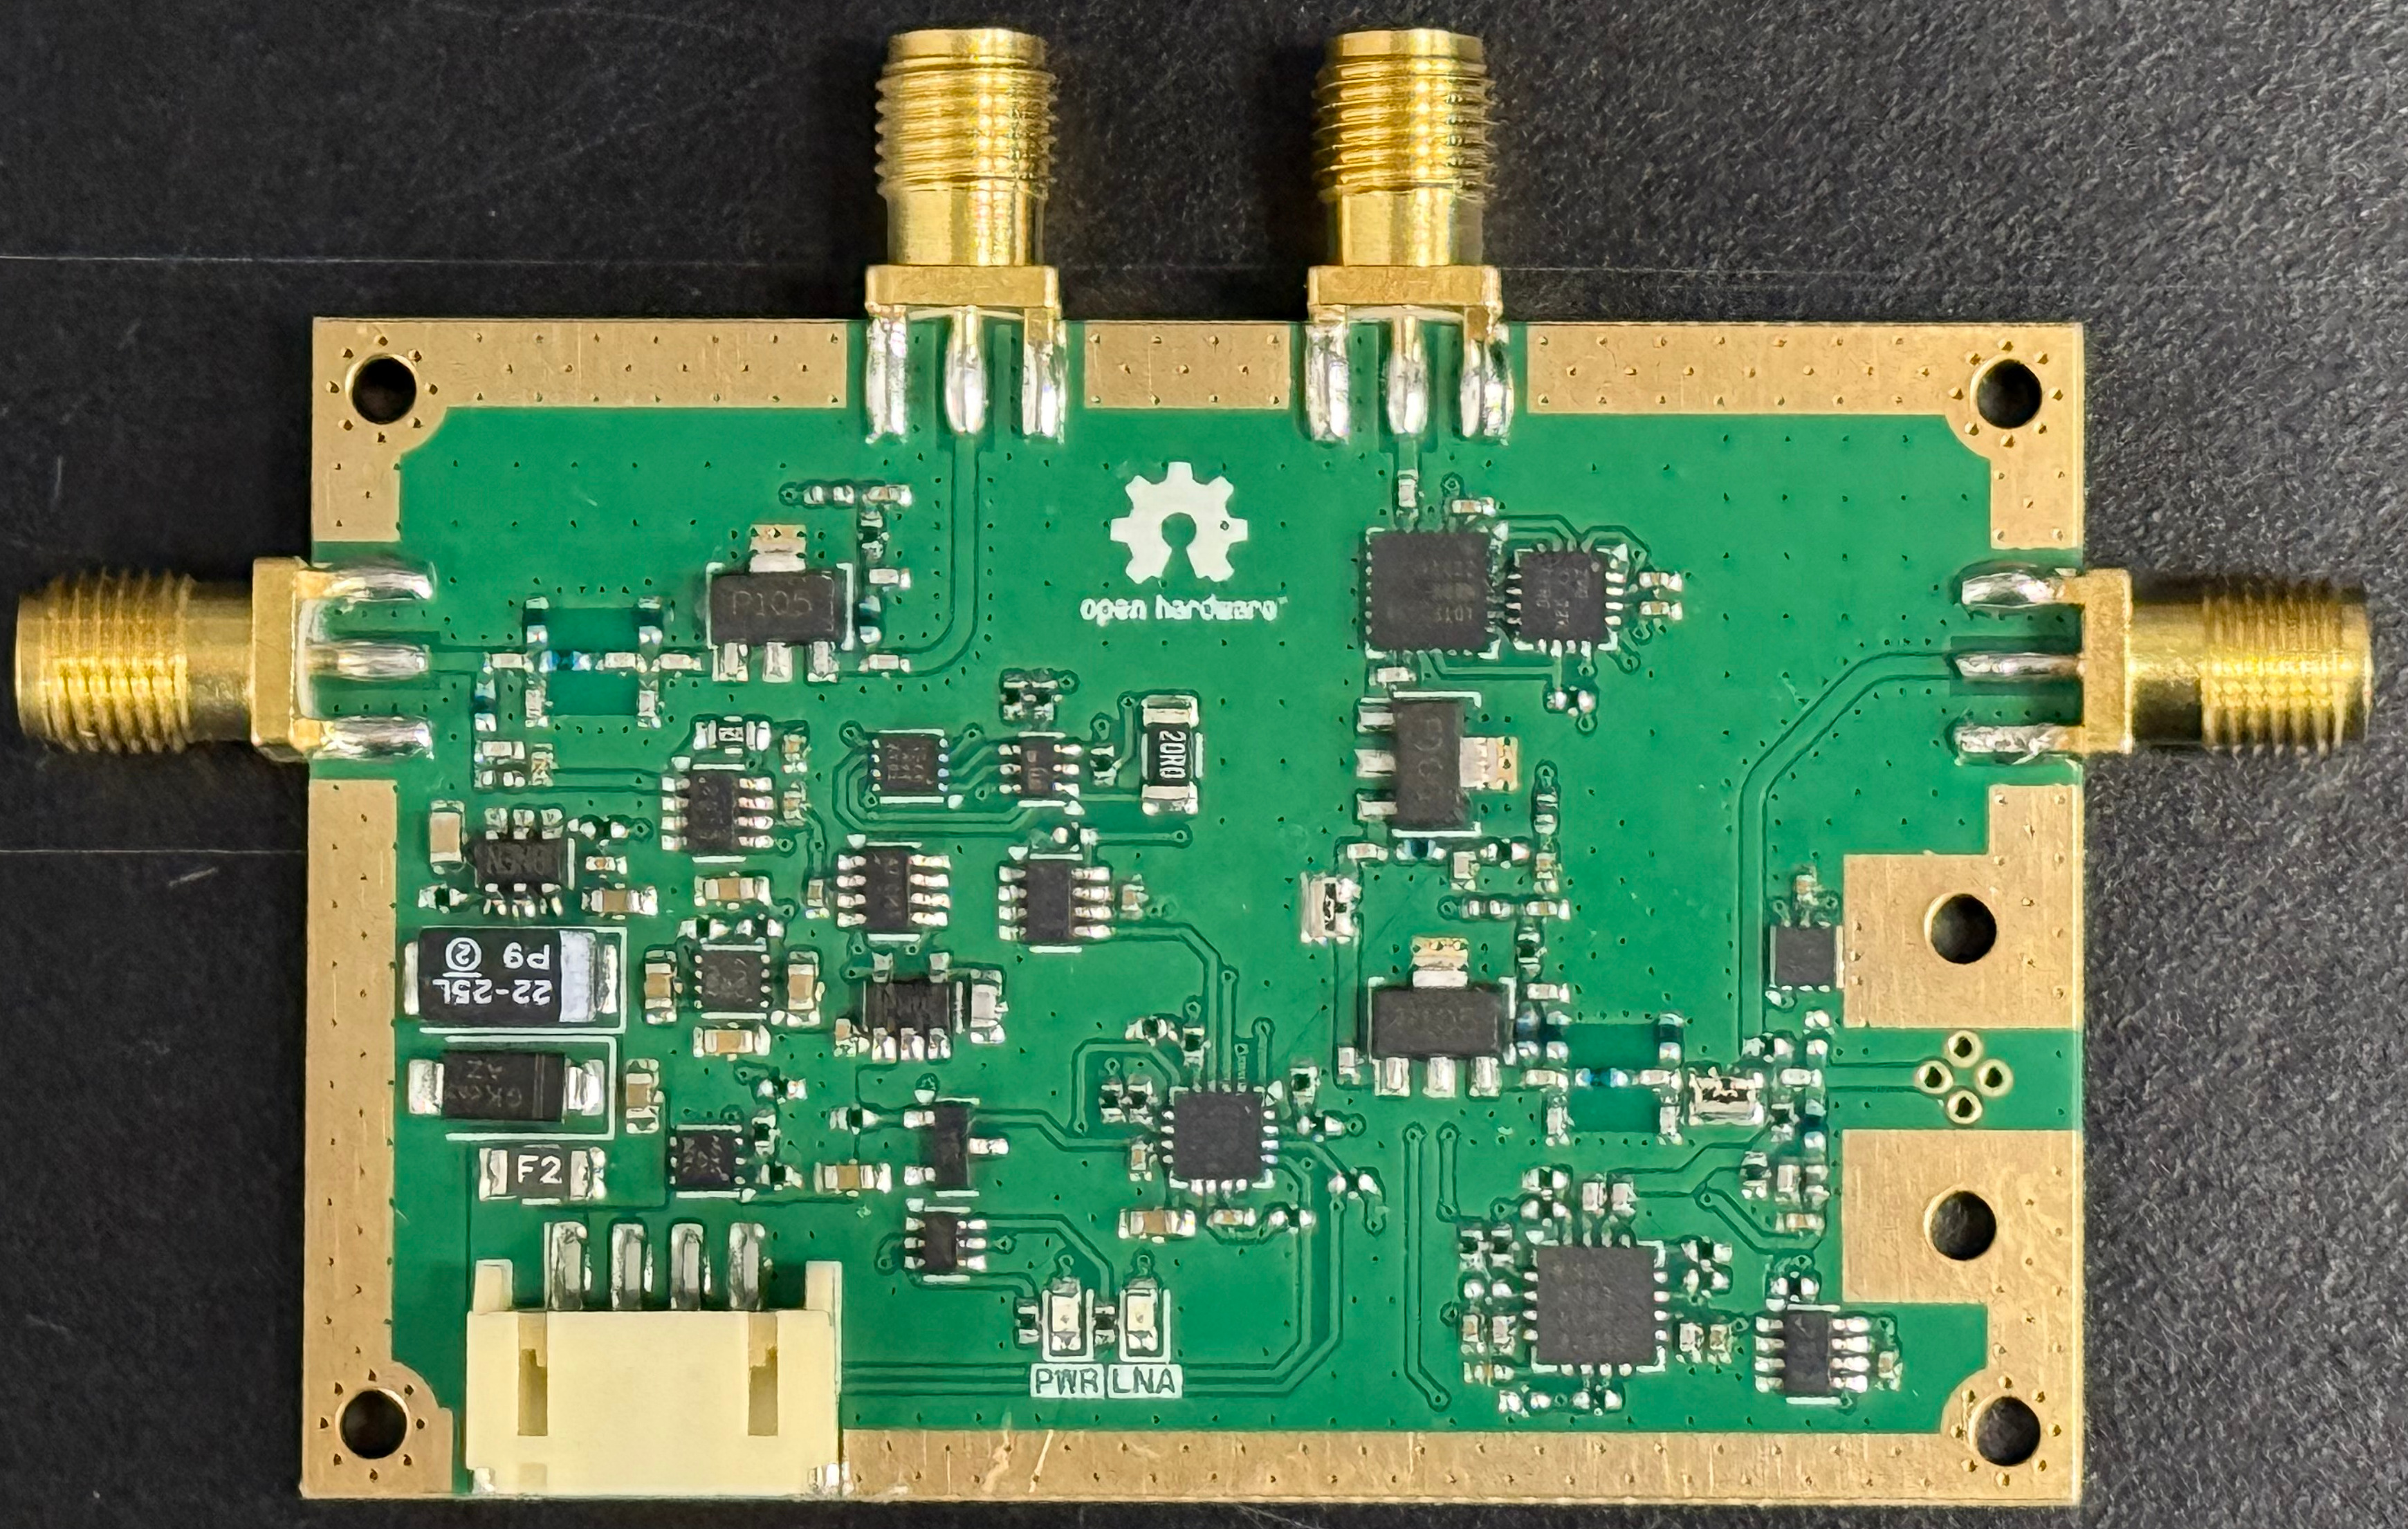
\includegraphics[height=4cm]{figures/ftx.jpg}}%
    \quad%
    \subfloat{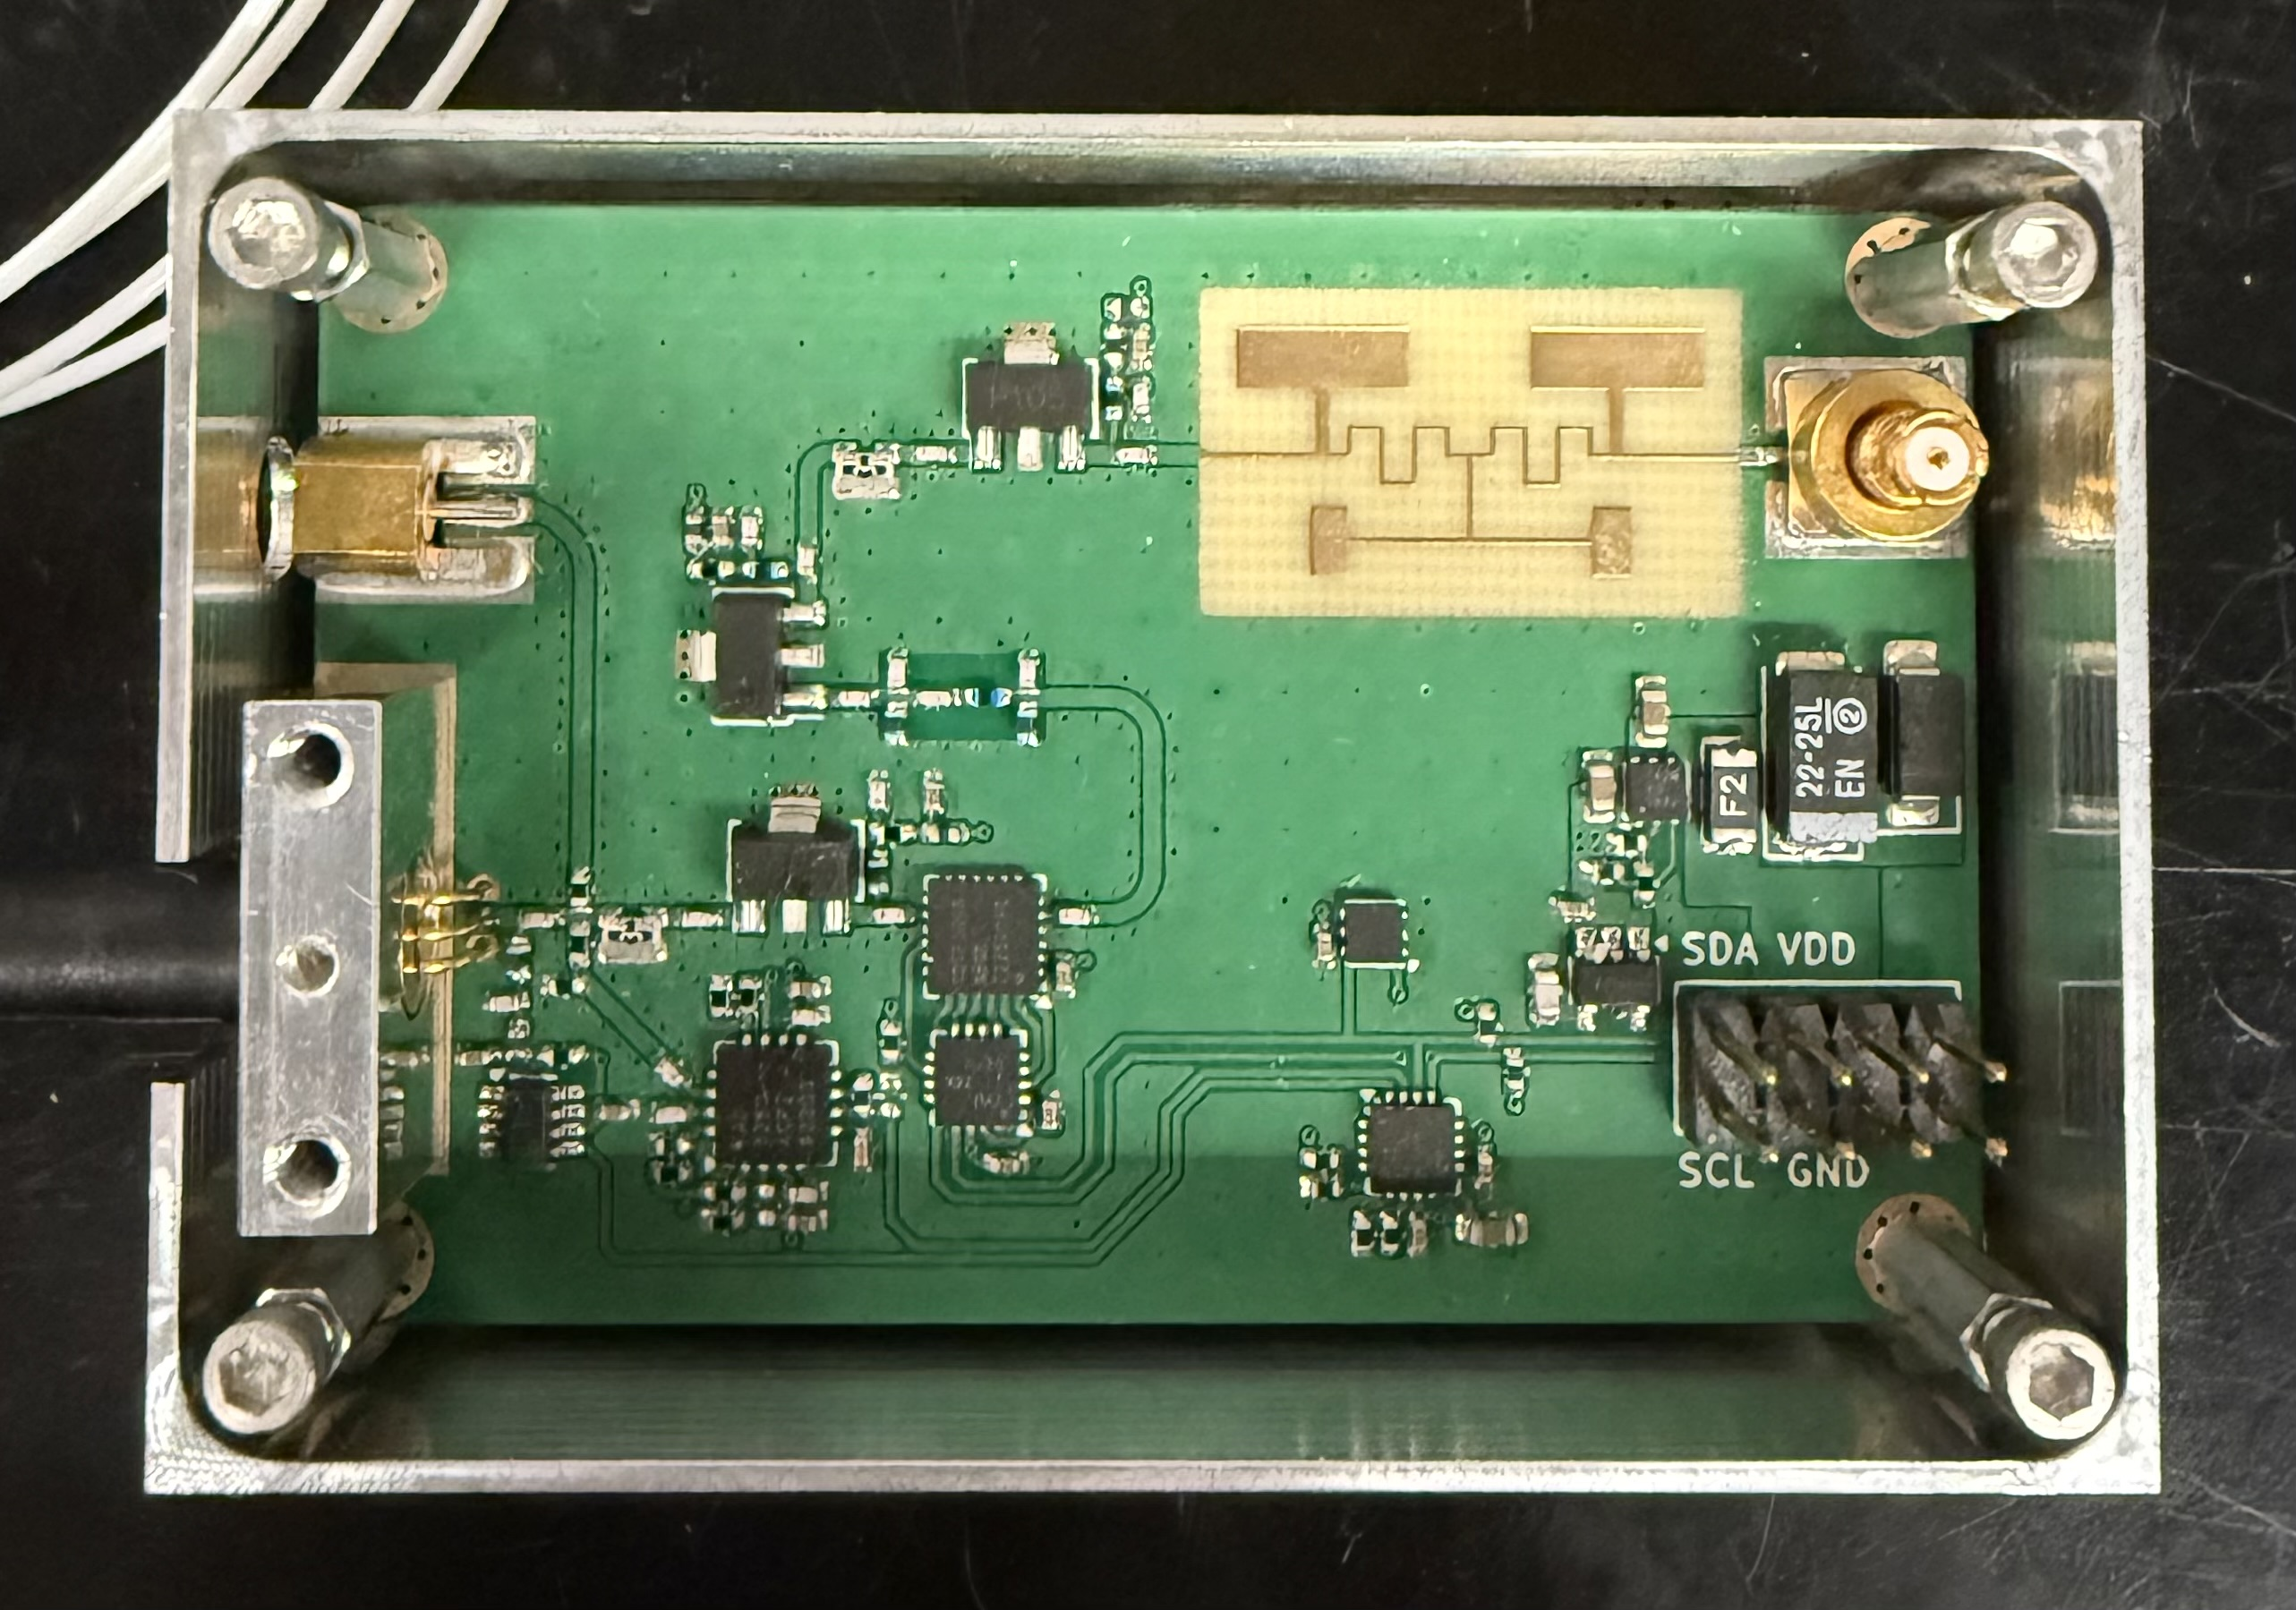
\includegraphics[height=4cm]{figures/frx.jpg}}%
    \caption{FTX and FRX PCBs}%
    \label{fig:ftx_frx}%
\end{figure}

To implement the analog signal path, we designed two printed circuit boards, shown in \autoref{fig:ftx_frx}.
These boards are the fiber transmitter (FTX) at the antenna station and the fiber receiver (FRX) at the central processing facility.
Both of these boards include monitor and control capabilities, measuring board currents, temperatures, and controlling digital step attenuators and bias currents.
This interface is achieved via an I$^2$C serial interface, whose digital lines are heavily filtered and will be disabled during observations.

\subsubsection{FTX}
The FTX board consists of three stages of amplification with a collection of filters and attenuators.
The laser bias is provided by a controlled current source, whose set point is controlled by a digital potentiometer.
The laser's anode is connected to the case, which implies we must drive the laser using a negative supply voltage.
Controlled current sources that allow for this are uncommon, motivating a custom design.
The design allows for a current selection between \qty{0}{\mA} and \qty{50}{\mA}, covering the full range of acceptable currents for the AGx laser.

In addition to the laser control, the FTX includes a connection point for an external filter.
In the current design stage, it is unclear if we will require much filtering besides shaping the 1280-1530 MHz bandpass.
In earlier stages of the project, strong interference causing significant distortion was a top concern.
The current RFI environment of the DSA-2000 site seems to indicate that no additional filtering will be required.
Nevertheless, the option to add the filters will remain if this situation changes.

The FTX board itself is housed inside an RFI-tight container, with feed-through connections for the RF, digital, and power signals.
The switching power supply for the board is housed on the outside of the enclosure to prevent switching noise from leaking into the signal path.
Each box contains electronics for both polarizations.

\subsubsection{FRX}

At the receiving side, the FRX module is a daughter board to the ``radio camera frontend'' or RCF.
The RCF is a larger card that hosts the ADCs and FPGA and fits into a 10-unit Eurocard subrack.
Two FRXes must then fit on a standard height card (\qty{100}{\mm}), with some gap for edge interfaces.
The RF signals out of the FRXes are connected to the digitizers on the RCF using a standard SMP board-to-board connector.
The FRXes are shielded with an aluminum cover that encloses the modules and are electrically connected to a ground plane on the RCF PCB.
The signals are routed on inner layers of the RCF PCB, so the FRX boards are surrounded by ground on all sides, except for a small slit that allows the fiber to exit.
The fiber pigtail is connected to the front panel of the card with a standard fiber interface.

The design of the FRX card was straightforward, with a standard assortment of filters and amplifiers.
Perhaps the most interesting component is the distributed low pass antialiasing filter at the output.
This filter is an inverse-Chebyshov low pass filter that has been optimized in physical area.
The center resonator was split in half and folded inwards to minimize space.

\section{LNA Improvements}

As the project progresses, the DSA-2000 team has been charged with pushing the performance even further, both in terms of what can be achieved before final design review and as avenues for future upgrades.
As the goal is to continue maximizing survey speed, we want to exhaust all options to reduce system noise within our budget.

For the current frequency range, there is very little we can do to improve the noise from a circuit design perspective.
The presented LNA from \autoref{ch:lna} is close to the theoretical minimum noise of the transistor, with typical losses of the matching network.
While this design is optimal for room temperature operation, it could benefit from cooling, as is the case for any transistor.
The entire premise of the ambient temperature LNA was to avoid cooling, but we can accomplish some cooling using Peltier microcoolers without resorting to expensive cryogenics.
Additionally, the noise of the amplifier is dependent on the source impedance presented by the feed.
As such, the design of the LNA input matching network could be modified to provide a better match to the feed instead of to \qty{50}{\ohm}.
The following section discusses these two potential improvements.

\subsection{Active Cooling}

Thermoelectric cooling of LNAs is a well-known approach~\cite{caoCoolingLowNoise2013} for improving an amplifier's noise.
However, most implementations of this strategy involve ``bulk'' cooling, where the entire amplifier assembly is cooled.
The power required for bulk cooling to achieve reasonable noise improvements can be significant.
Additionally, the hot-side of the cooler would need a large heat sink and fan for thermal management, adding size, weight, and power.
An alternative for hybrid amplifiers is to cool only the first-stage transistor, as that has the highest impact on the LNA's noise.
These transistors are very small and low power, requiring significantly less cooler power than what would be required to achieve the same noise improvement in bulk cooling.
Modern advancements in miniaturization of Peltier coolers for optoelectronics\footnote{Typically used for lasers in high-speed digital communication} have dramatically lowered cost and improved performance.
As such, we have designed an amplifier with an embedded microcooler for the first stage transistor to improve the noise without significant impact to cost or power consumption.
Variants on this idea have been shown before~\cite{schreuderLocalizedLNAVooling2006}, but have been limited to MMIC-based amplifiers, which require a larger cold-side area and cooling capacity.

The potential noise gains, however, need to be weighed against the complications that could arise due to creating a below-freezing point inside the amplifier.
This presents a formidable design challenge, as the goal for the project is to have an exceptionally low mean-time-to-failure.
If water vapor were to leak into the chassis, it would freeze over the transistor and result in failures.
To prevent this, we need to design an LNA that is hermetically sealed, which adds complexity and cost.
The improvement in survey speed, however, could be substantial depending on what is achievable and may outweigh the added engineering costs.

The current LNA design biases the transistor at a power of \qty{8}{\mW} (\qty{0.5}{\V} at \qty{16}{\mA} of drain current).
Models for this transistor at \qty{2}{\GHz} indicate a minimum noise temperature of \qty{7}{\K} at \qty{300}{\K} ambient and \qty{0.6}{\K} at \qty{15}{\K} ambient.
This results in a noise slope of about \qty{1}{\K} per \qty{45}{\K} change in ambient temperature.
To improve our amplifier by \qty{1}{\K}, we can integrate a small single-stage microcooler to generate the \qty{45}{\K} differential.

To fully estimate the heat load that we would need to cool, we must account for heat introduced from the short wire bonds.
We can compute this via
\begin{equation}
    Q_\text{Wires} = NK\frac{S}{L}\Delta T \,,
\end{equation}
where $N$ is the number of wires, $K$ is the wire material thermal conductivity, $S$ is the wire cross-sectional area, $L$ is the wire length, and $\Delta T$ is the temperature differential.
If we require $N=$ \num{5}, \qty{20}{\micro\m} diameter ($S$ \qty{=2.54e-10}{\m^2}) wire bonds (three for the transistor and two for the thermistor) made of gold ($K$ \qty{=314}{\W\per\m\per\K}) with an average length of $L$ \qty{=500}{\micro\m} across the $\Delta T$ of \qty{45}{\K}, we have an additional heat load of \qty{36}{\mW}.
This implies that the bulk of the required cooling capacity comes from the wire bonds and not the transistor.

As the $\Delta T$ produced by a Peltier cooler behaves non-linearly under different heat loads, a bit of trial and error is required to estimate their performance properly.
Estimations from the manufacturer\urlfootnote{https://www.tec-microsystems.com/} for their \texttt{1TC22-0044-25.H} model predicts a maximum $\Delta T$ of just beneath \qty{30}{\K} for \qty{45}{\mW} of heat.
With this $\Delta T$, however, the cooling requirement will be smaller as the heat from the wire bonds is less due to the lower temperature differential.
In this scenario, we can compute a total wire bond head load of \qty{32}{\mW}, which would induce a new $\Delta T$ closer to \qty{40}{\K}.
This all implies we can expect a measured $\Delta T$ of between \qty{30}{\K} and \qty{40}{\K}.

\begin{figure}[ht!]%
    \centering
    \subfloat{
        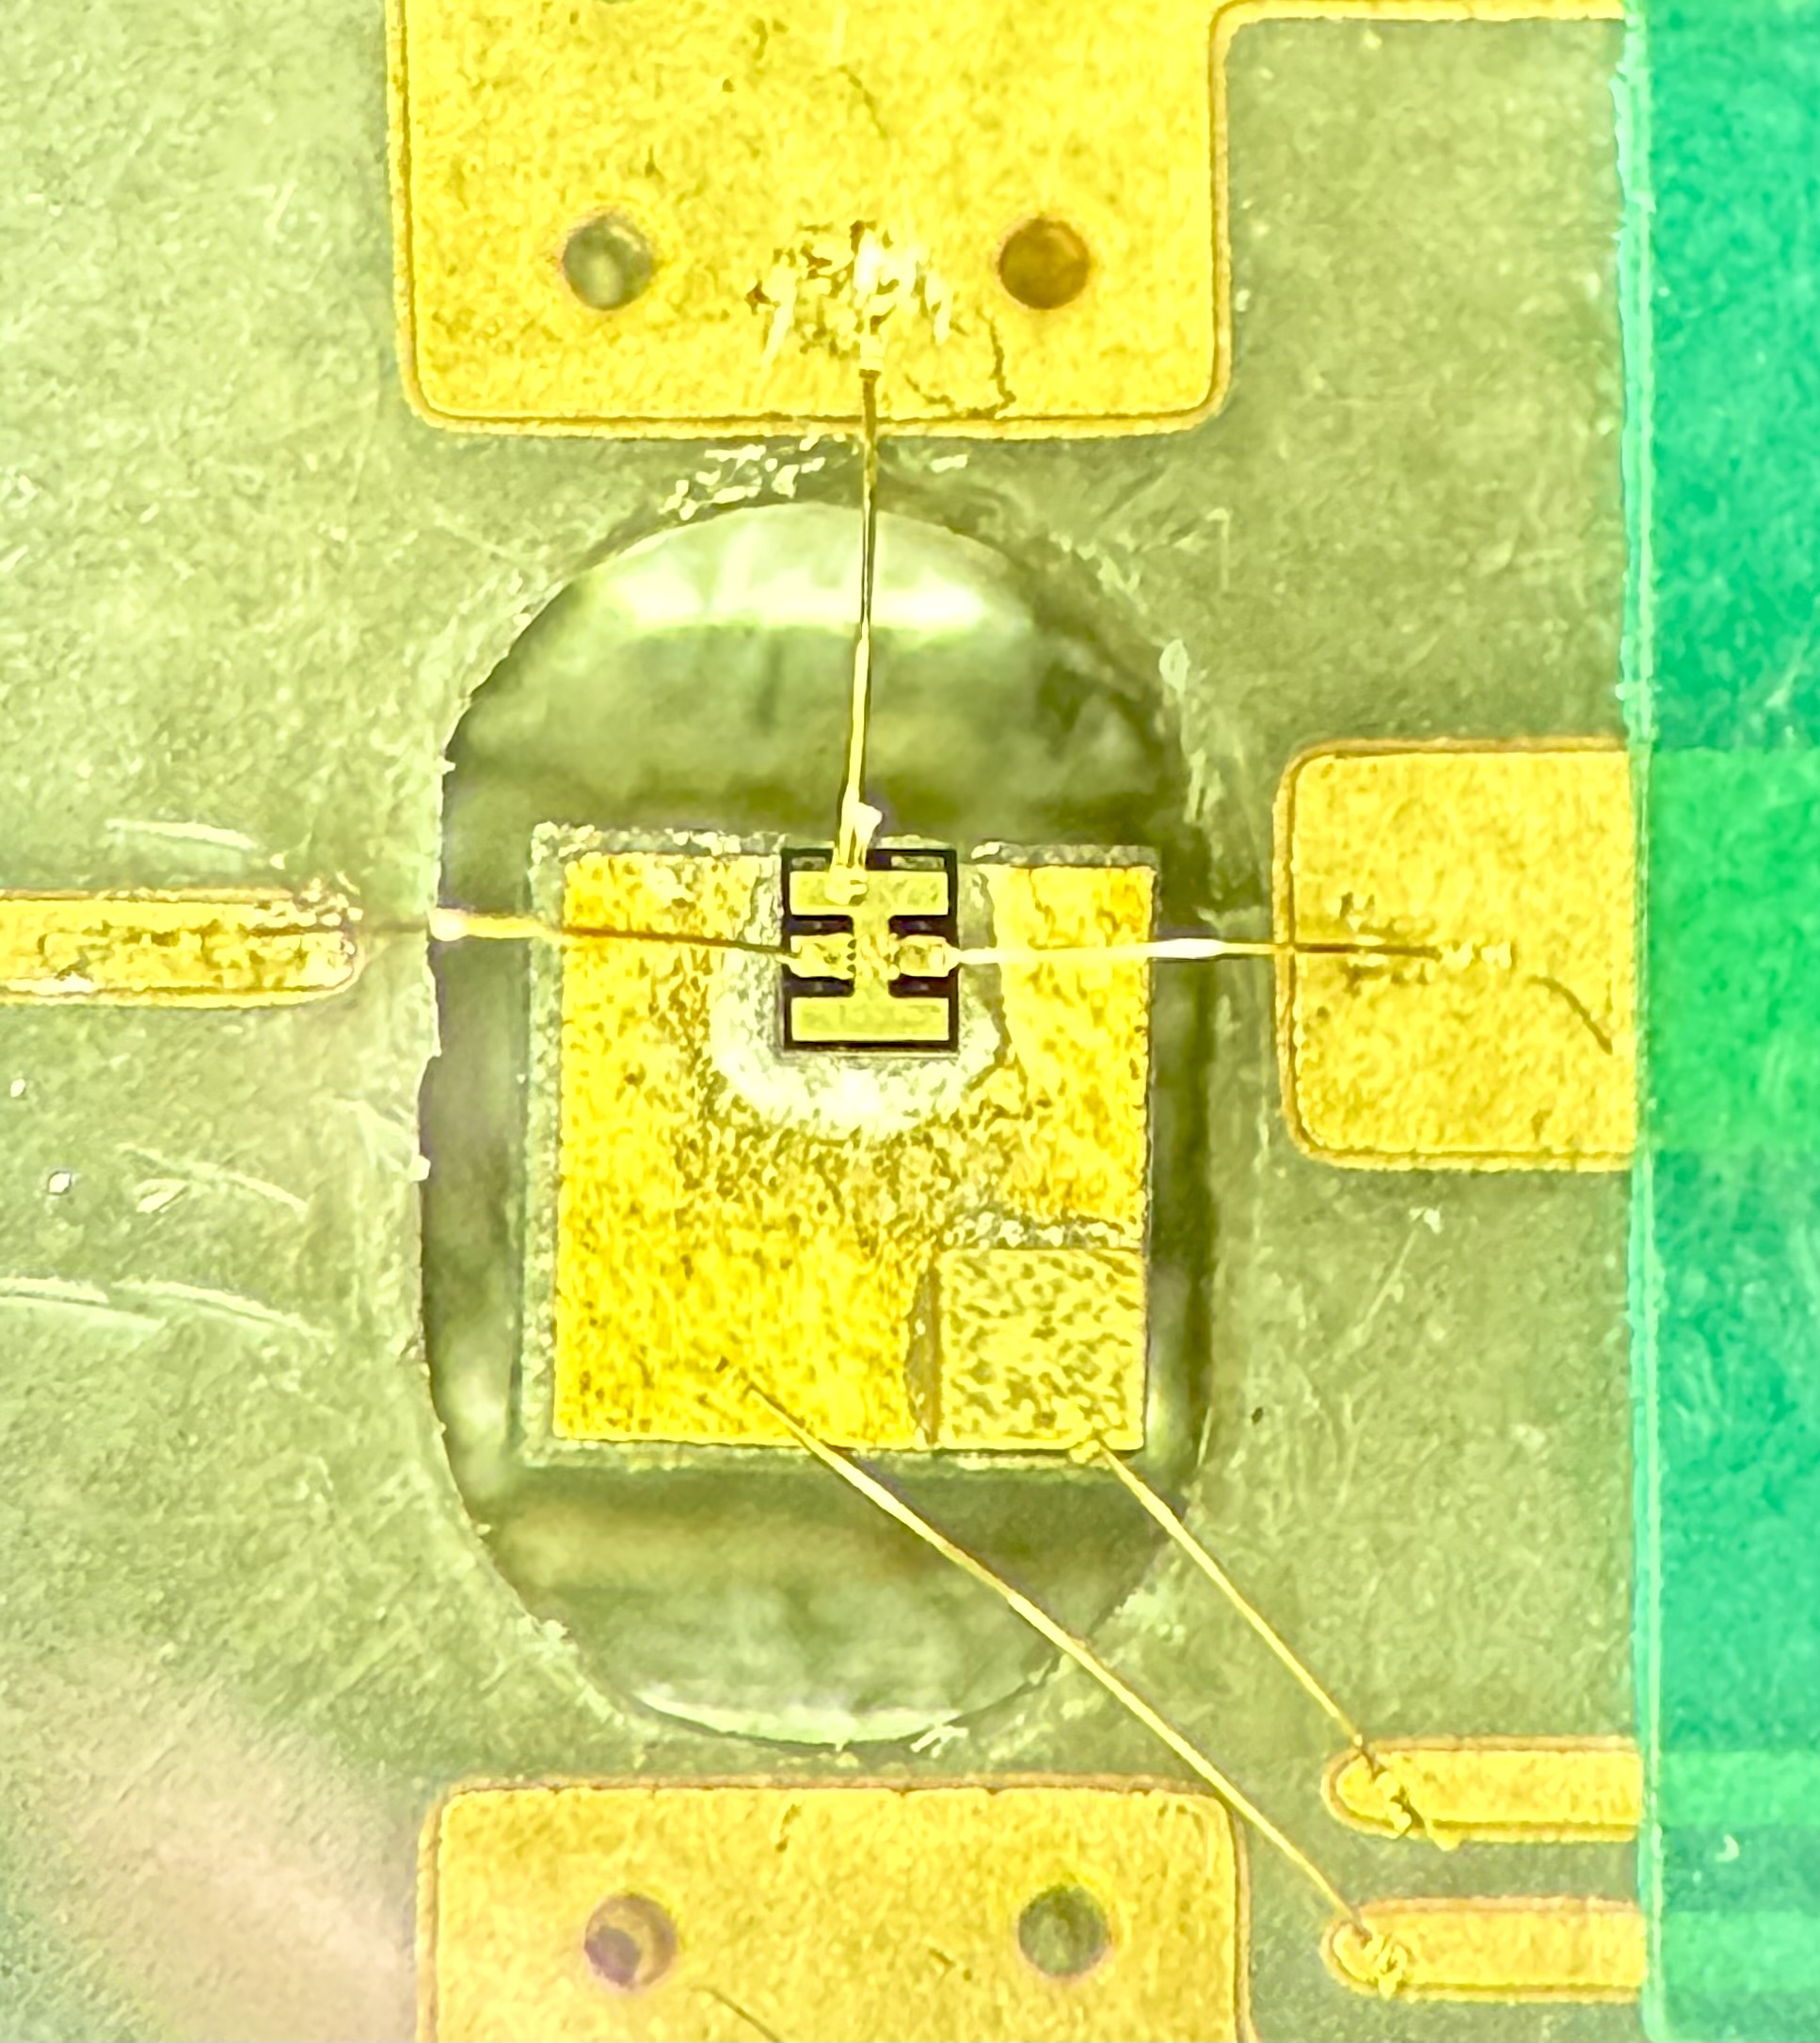
\includegraphics[height=6cm]{figures/tec.jpg}
    }
    \subfloat{
        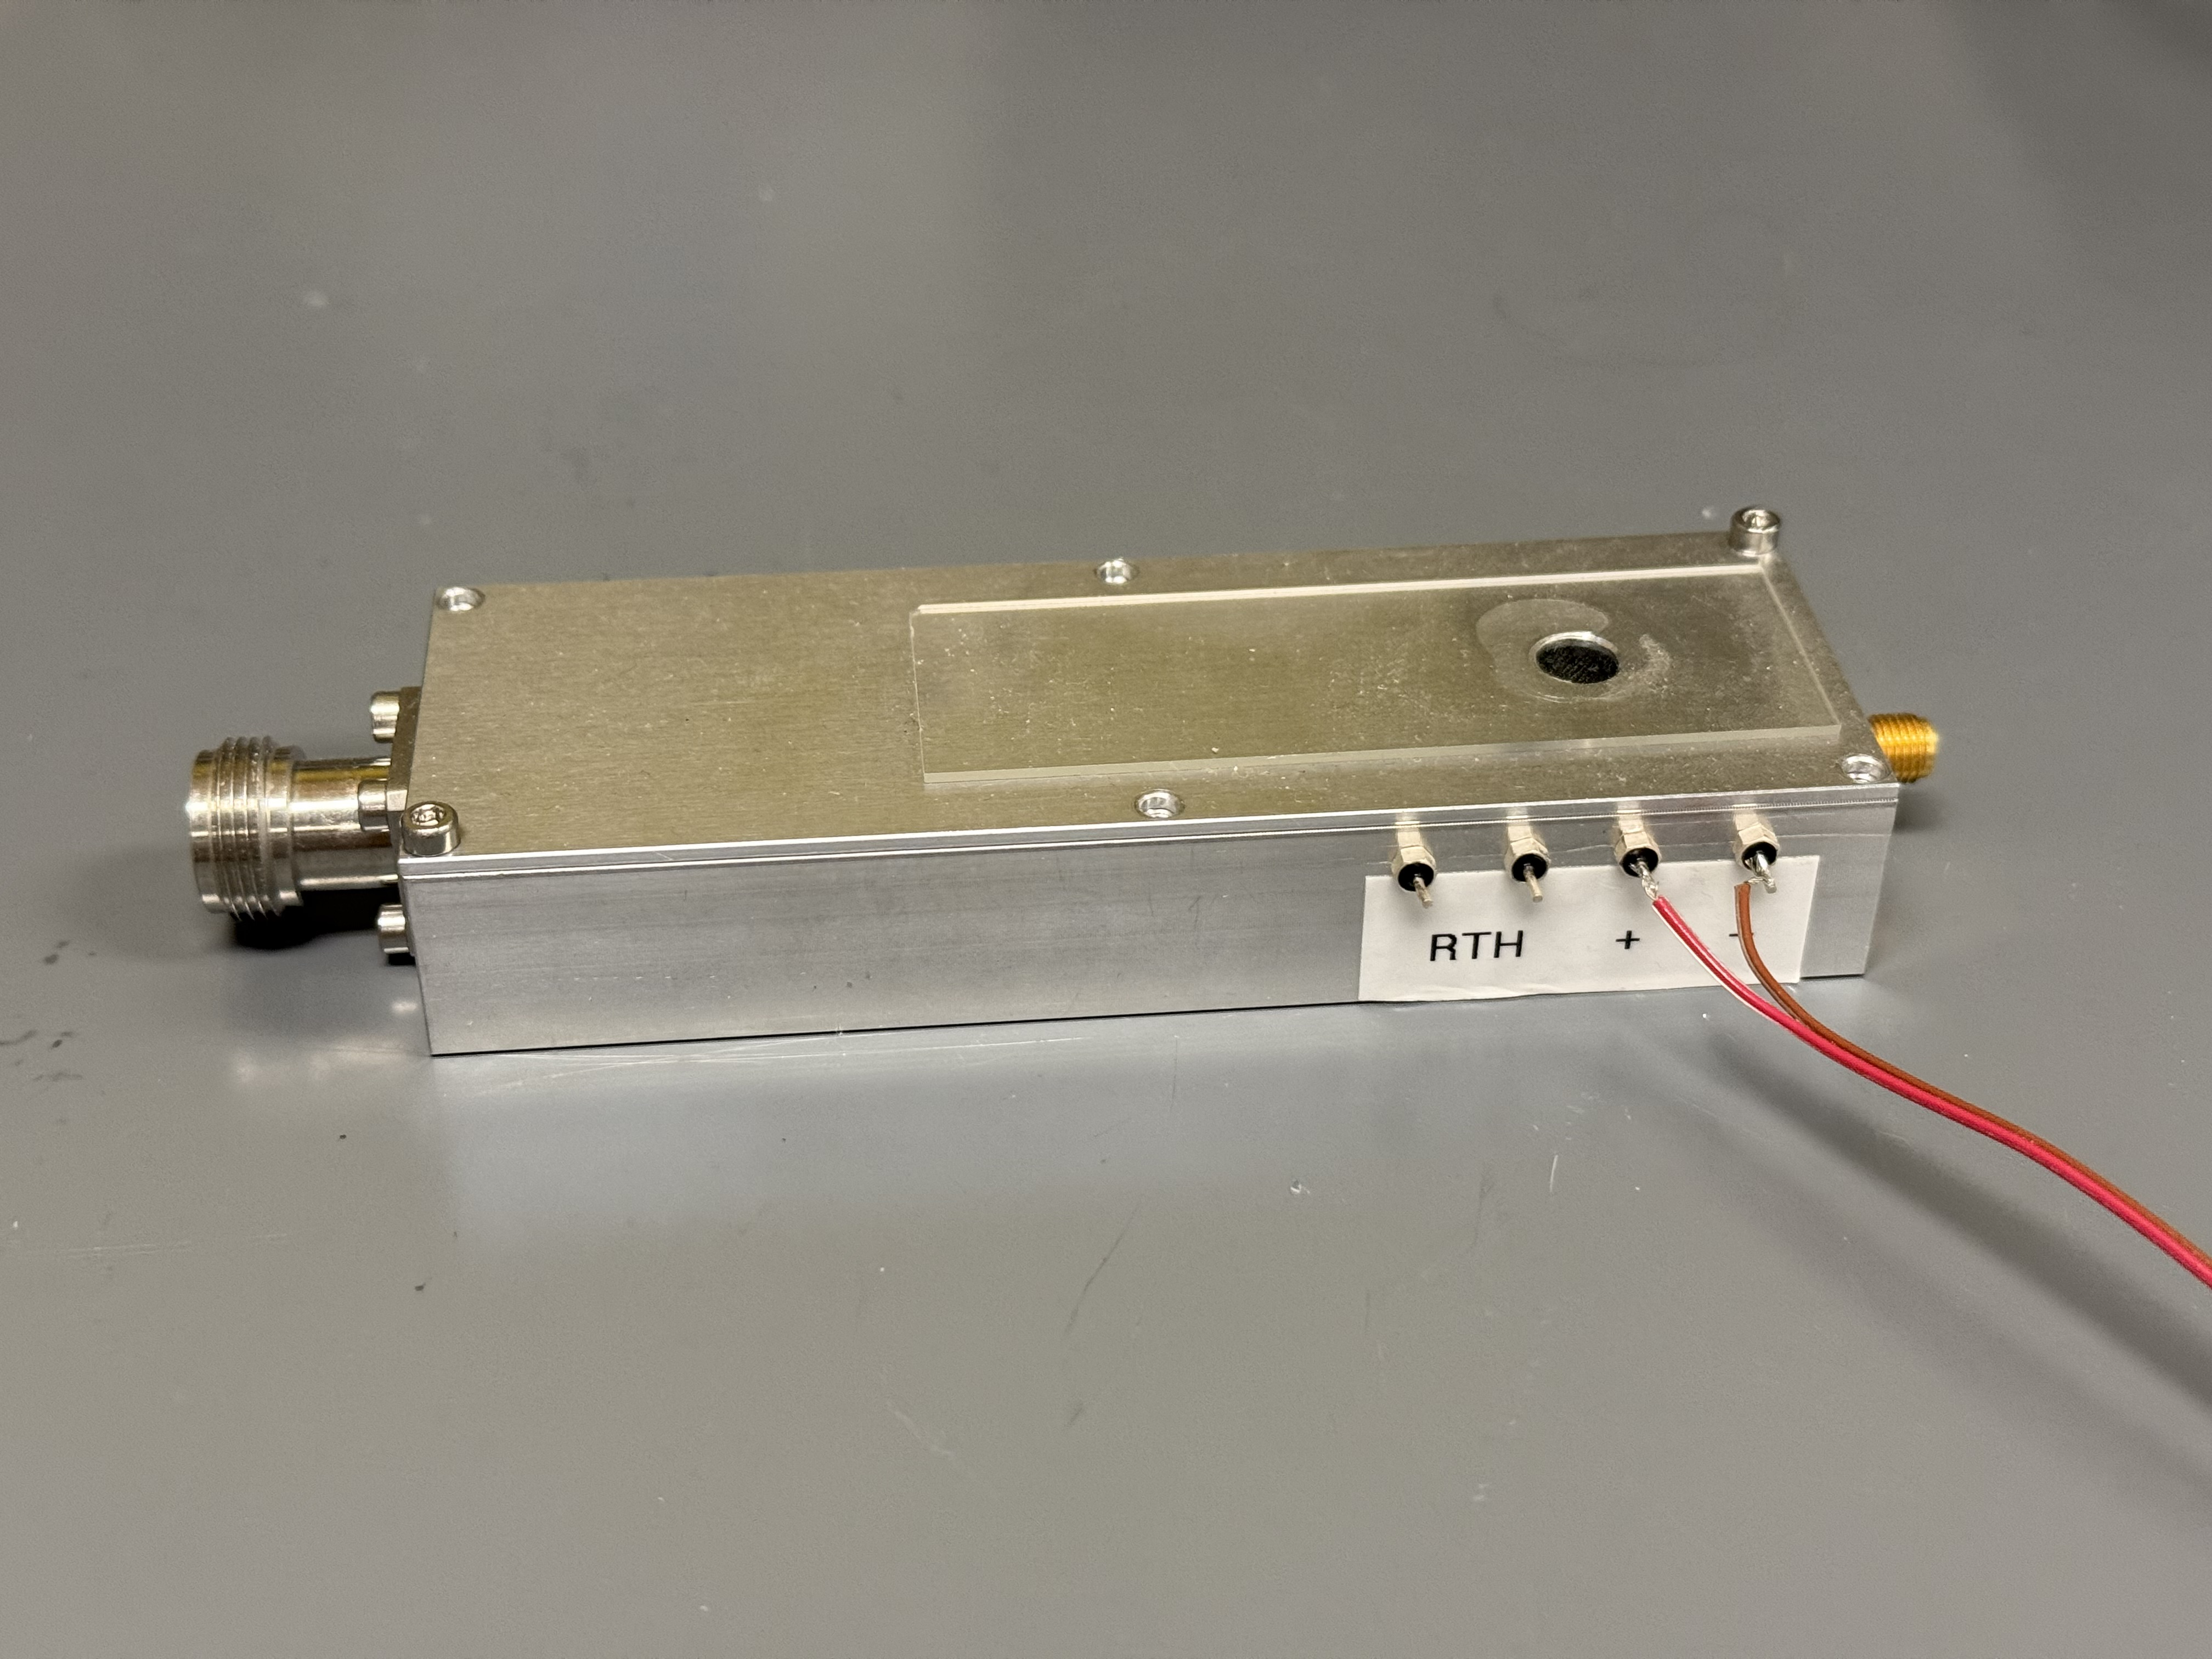
\includegraphics[height=6cm]{figures/cooled_amp.jpg}
    }%
    \caption{Bonded transistor on microcooler and constructed cooled amplifier}
    \label{fig:lna_cooling}%
\end{figure}

We constructed a copy of the amplifier described in \autoref{ch:lna}, but with an embedded microcooler.
While this amplifier was not hermetically sealed, two holes were added at either end, with dry nitrogen pumped through one side.
Additionally, a hole and microscope slide was added to the lid to observe the first stage transistor under cooling to watch for ice formation.
The microcooler was powered via an independent supply, and a thermistor was mounted to the cold-stage, adjacent to the transistor to monitor the temperature.
Finally, we performed the precision noise measurement described in \autoref{ch:lna}.
A close-up picture of the bonded transistor (center) and thermistor (bottom right) on the microcooler and assembled amplifier is shown in \autoref{fig:lna_cooling}.
The transistor's wire bonds from left to right are the gate, source, and drain.

With zero power applied to the microcooler, we measured a thermistor temperature of \qty{30}{\C}.
With the cooler powered to its maximum current, we measured a thermistor temperature of \qty{-10}{\C}, for a $\Delta T$ of \qty{40}{C}.
The LNA noise temperature dropped by an average of about \qty{0.75}{\K}, shown in \autoref{fig:cooled_noise}, which is very close to the predicted \qty{0.89}{\K} and well within the error for this measurement.

While the experiment was a success, eventually ice did start to form on the first stage transistor, destroying the fragile air bridges.
Work on this solid-state cooling approach needs further investigation in environmental control, especially as it pertains to mass-manufacture for the 4000 LNAs that would eventually need to be built.
Additionally, our original estimations of the heat load which influenced the sizing of the microcooler did not include the heat load of the wire bonds.
The manufacturer has suggested a new custom part, \texttt{1TC22-0040-21.H}, which should have a higher $\Delta T$ of about \qty{50}{\K} under our heat load of \qty{\approx40}{\mW}.
We could also investigate two-stage coolers for significantly more cooling capacity, but with a downside of doubling the cross-sectional area of the cold-stage.
This would increase wire bond length which would reduce the heat load, but add significant inductance which will alter our matching network.

\newpage

\begin{figure}[ht!]
    \centering
    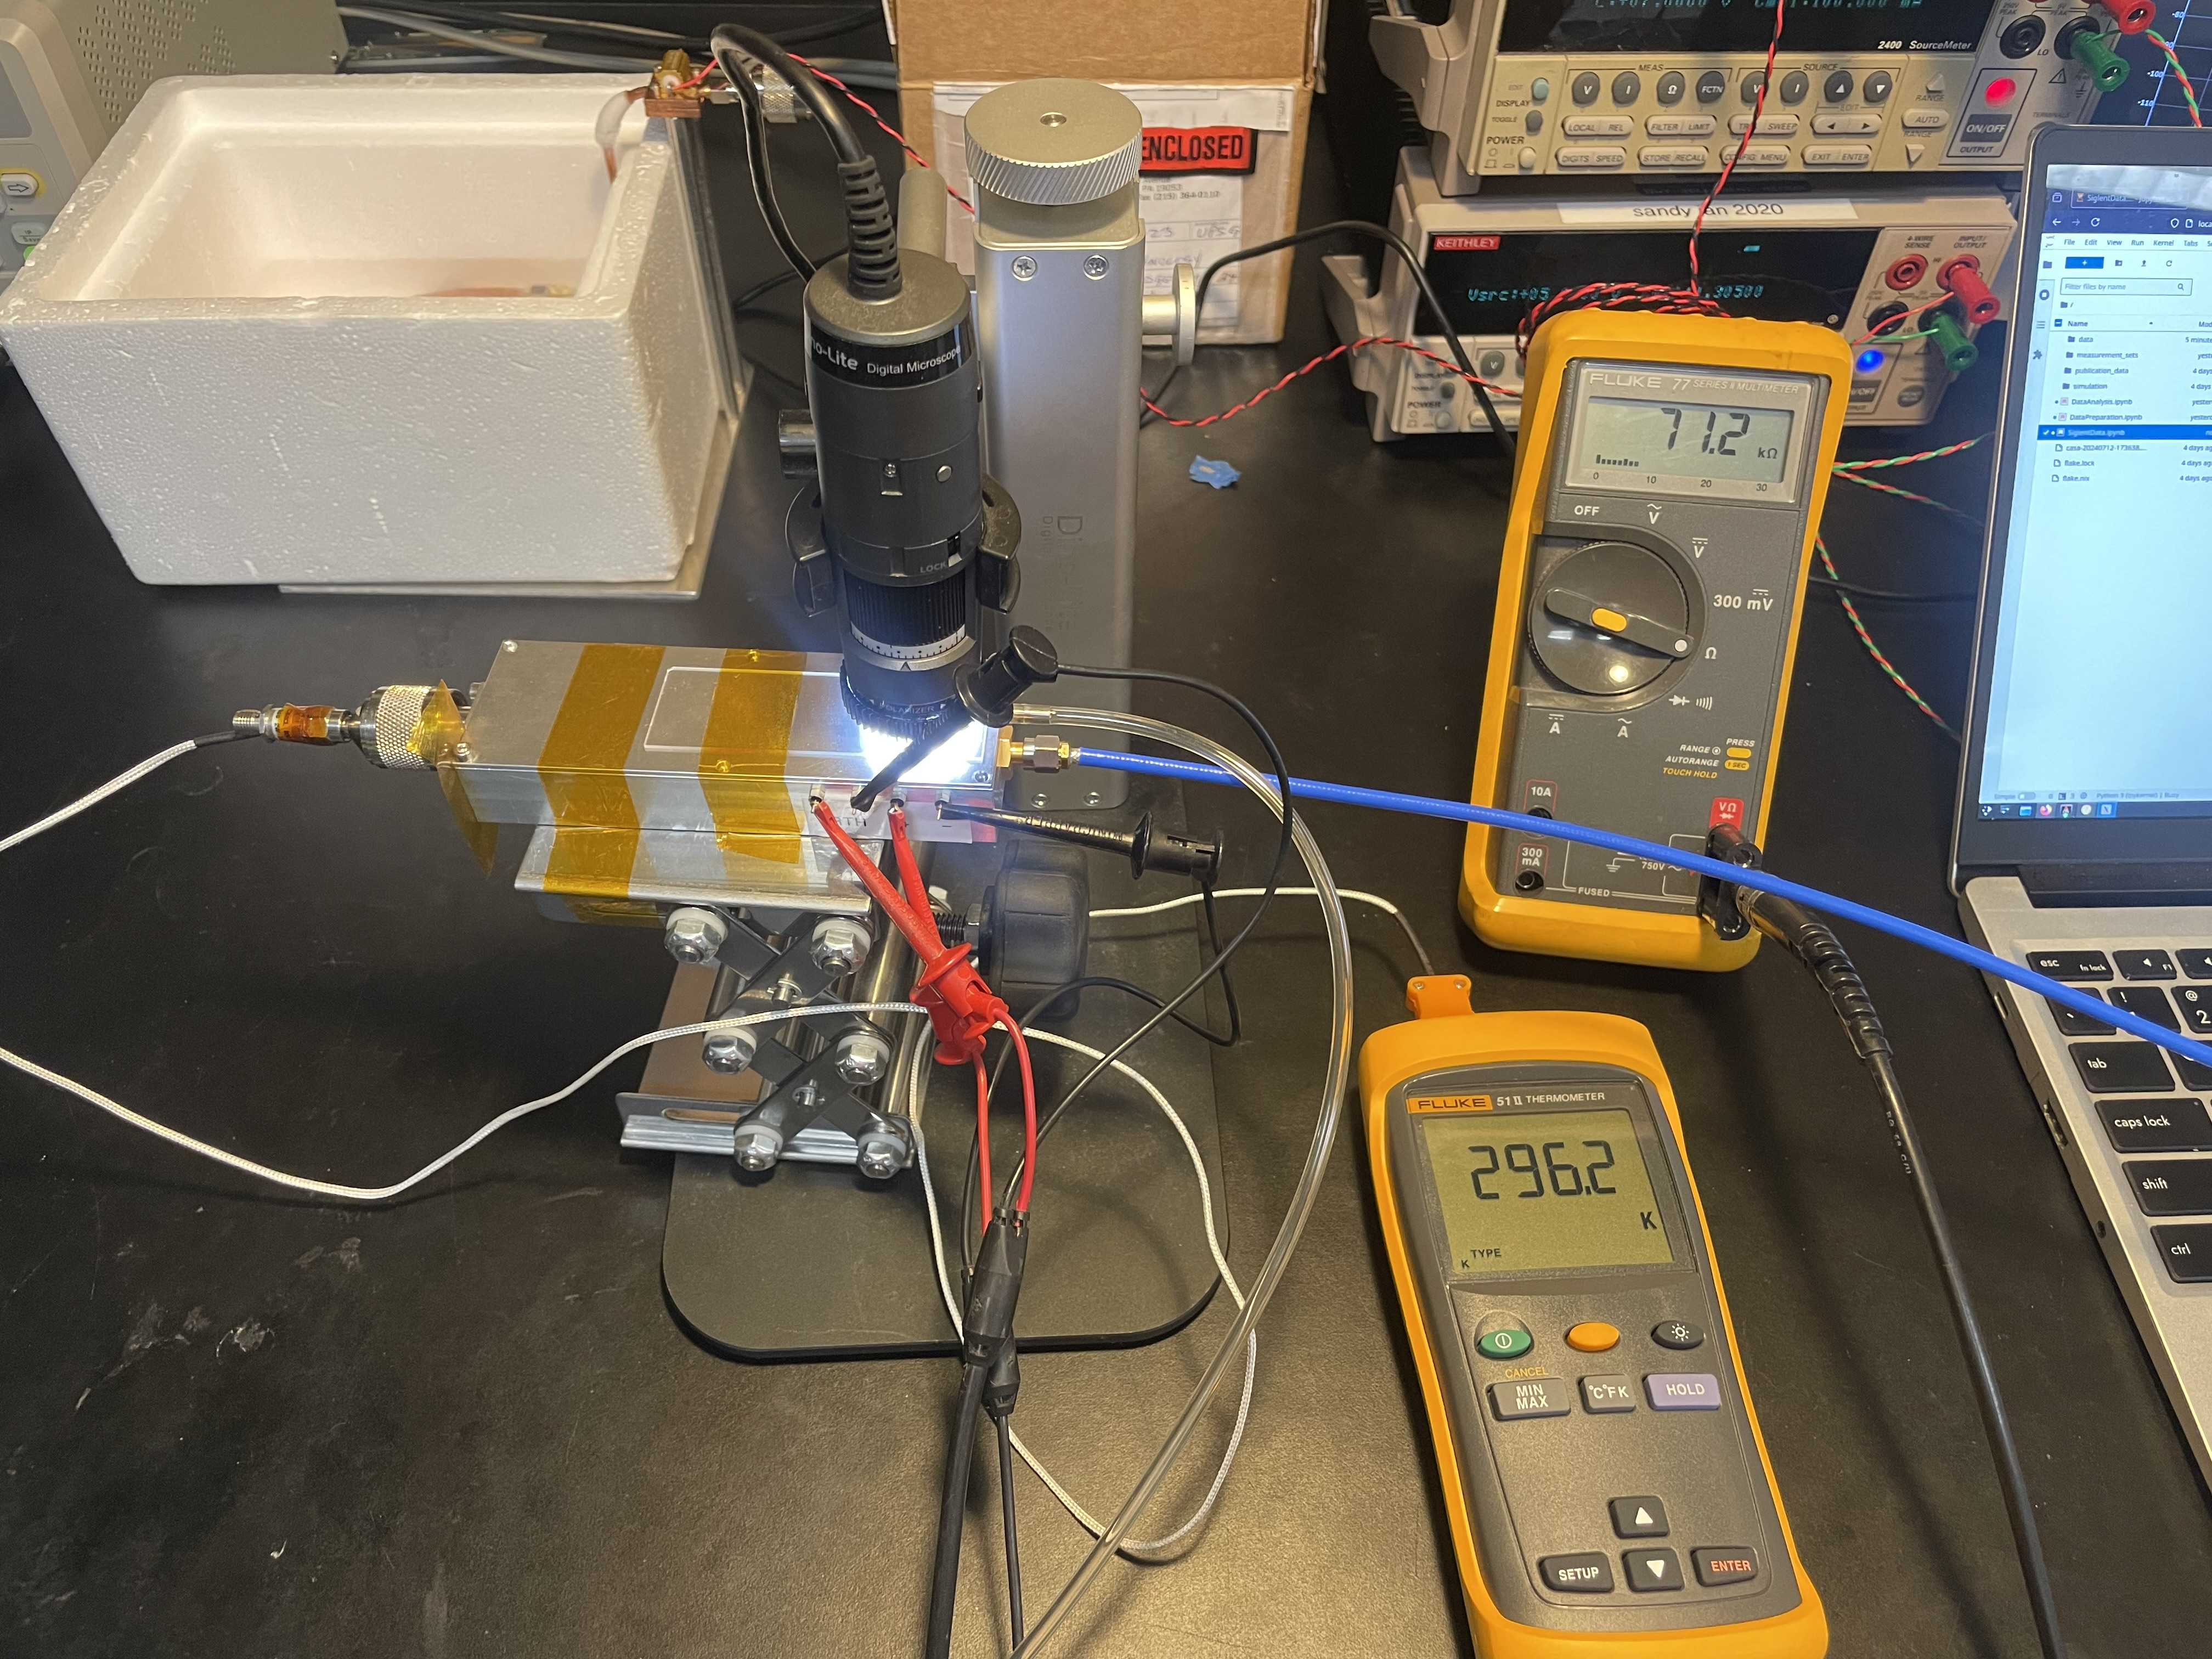
\includegraphics[width=0.8\linewidth]{figures/noise_test.jpg}
    \caption{Test setup for cooled amplifier noise measurements}
    \label{fig:noise_test}
\end{figure}

\begin{figure}[ht!]
    \centering
    \includestandalone[mode=buildnew]{figures/cooled_noise}
    \caption{Measured noise temperature of cooled amplifier}
    \label{fig:cooled_noise}
\end{figure}

\newpage

\subsection{Optimization of LNA Input Matching Network to Feed Impedance}

All our amplifier designs up to this point are intended to operate in a \qty{50}{\ohm} system, but the impedance presented by the feed is not \qty{50}{\ohm}.
The feed has return loss greater than \qty{10}{\dB} over much of the band, but the mismatch at the band edges significantly degrades the noise.

To reduce the effect of the feed impedance ``pulling'' the noise, we can design a matching network that is optimized for the feed impedance.
If the feed impedance were a large deviation from \qty{50}{\ohm}, it would be difficult to validate performance in the lab, as all the noise experiments are done in a \qty{50}{\ohm} system.
However, as the feed was intended to match to \qty{50}{\ohm}, we only have to compensate for a small difference in impedance, leaving the \qty{50}{\ohm} bench test more than satisfactory for validating performance.

Performing the co-optimization follows the work from \autoref{ch:lna}, with a small modification made to the definition of the noise goal in the cost expression.
Before, we were simply using $S_{22}$ of the nonuniform input matching network as the source reflection coefficient $\Gamma_S$ needed to compute the noise via \autoref{eq:noise_f}.
Now, we take measured $S_{11}$ data of the feed and compute $\Gamma_\text{Out}$ via
\begin{equation}
    \Gamma_\text{Out} = S_{22} + \frac{S_{21}S_{12}\Gamma_S}{1 - S_{11}\Gamma_S} \,,
\end{equation}
where $\Gamma_S$ is the measured feed $S_{11}$ (assuming everything is normalized to the same reference impedance).

The current feed design~\cite{flygareWidebandFeedReflector2023, flygareWidebandLowLossFeed2024}, is a quad-ridge flared horn, following previous work at Caltech~\cite{akgirayNewTechnologiesDriving2013}.
This feed includes a dielectric lens and ``cake pan'' choke rings to optimize the illumination of the DSA-2000 reflector.
As the ridges form a balanced transmission line, there is a shorted-pin balun that transitions from coax.
This transition is then brought to the edge of the feed structure to a standard microwave connector.
In the current design, the LNA is attached directly to this connector, resulting in the feed and LNA as two separate line-replaceable units (LRUs).

While the separation of components is useful from a maintenance perspective, the long coax pin that attaches the connector to the throat of the feed introduces additional loss.
An alternative design is to embed the LNA into the feed, using the ridge as the enclosure for the LNA PCB.
This sidesteps the need for the long coax pin and allows us to start the matching network very close to the slotline transition.
We can accomplish this while maintaining two distinct LRUs by designing an LNA chassis that slots into the ridge and connects to a blind-mate pin.
The new LNA chassis has a silver-epoxied \qty{50}{\ohm} glass feed-through connector to connect to the internal blind-mate pin.
A lid gasket and hermetic output connector seal the assembly and allow for solid-state cooling.

\begin{figure}[ht!]
    \centering
    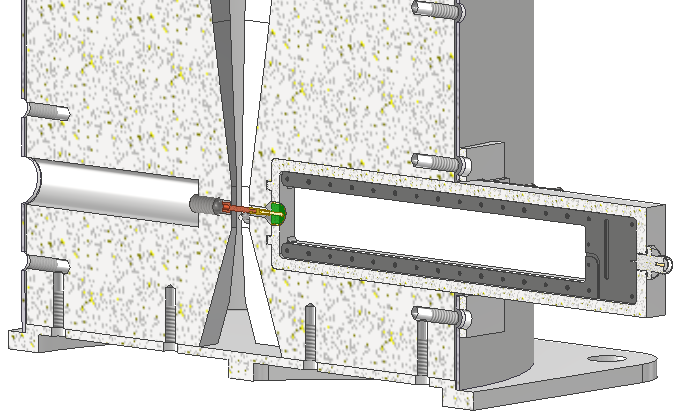
\includegraphics[width=\linewidth]{figures/feed_embed_cross_section.png}
    \caption{Cross-section of an LNA-embedded feed}
    \label{fig:feed_and_lna}
\end{figure}

\begin{figure}[ht!]
    \centering
    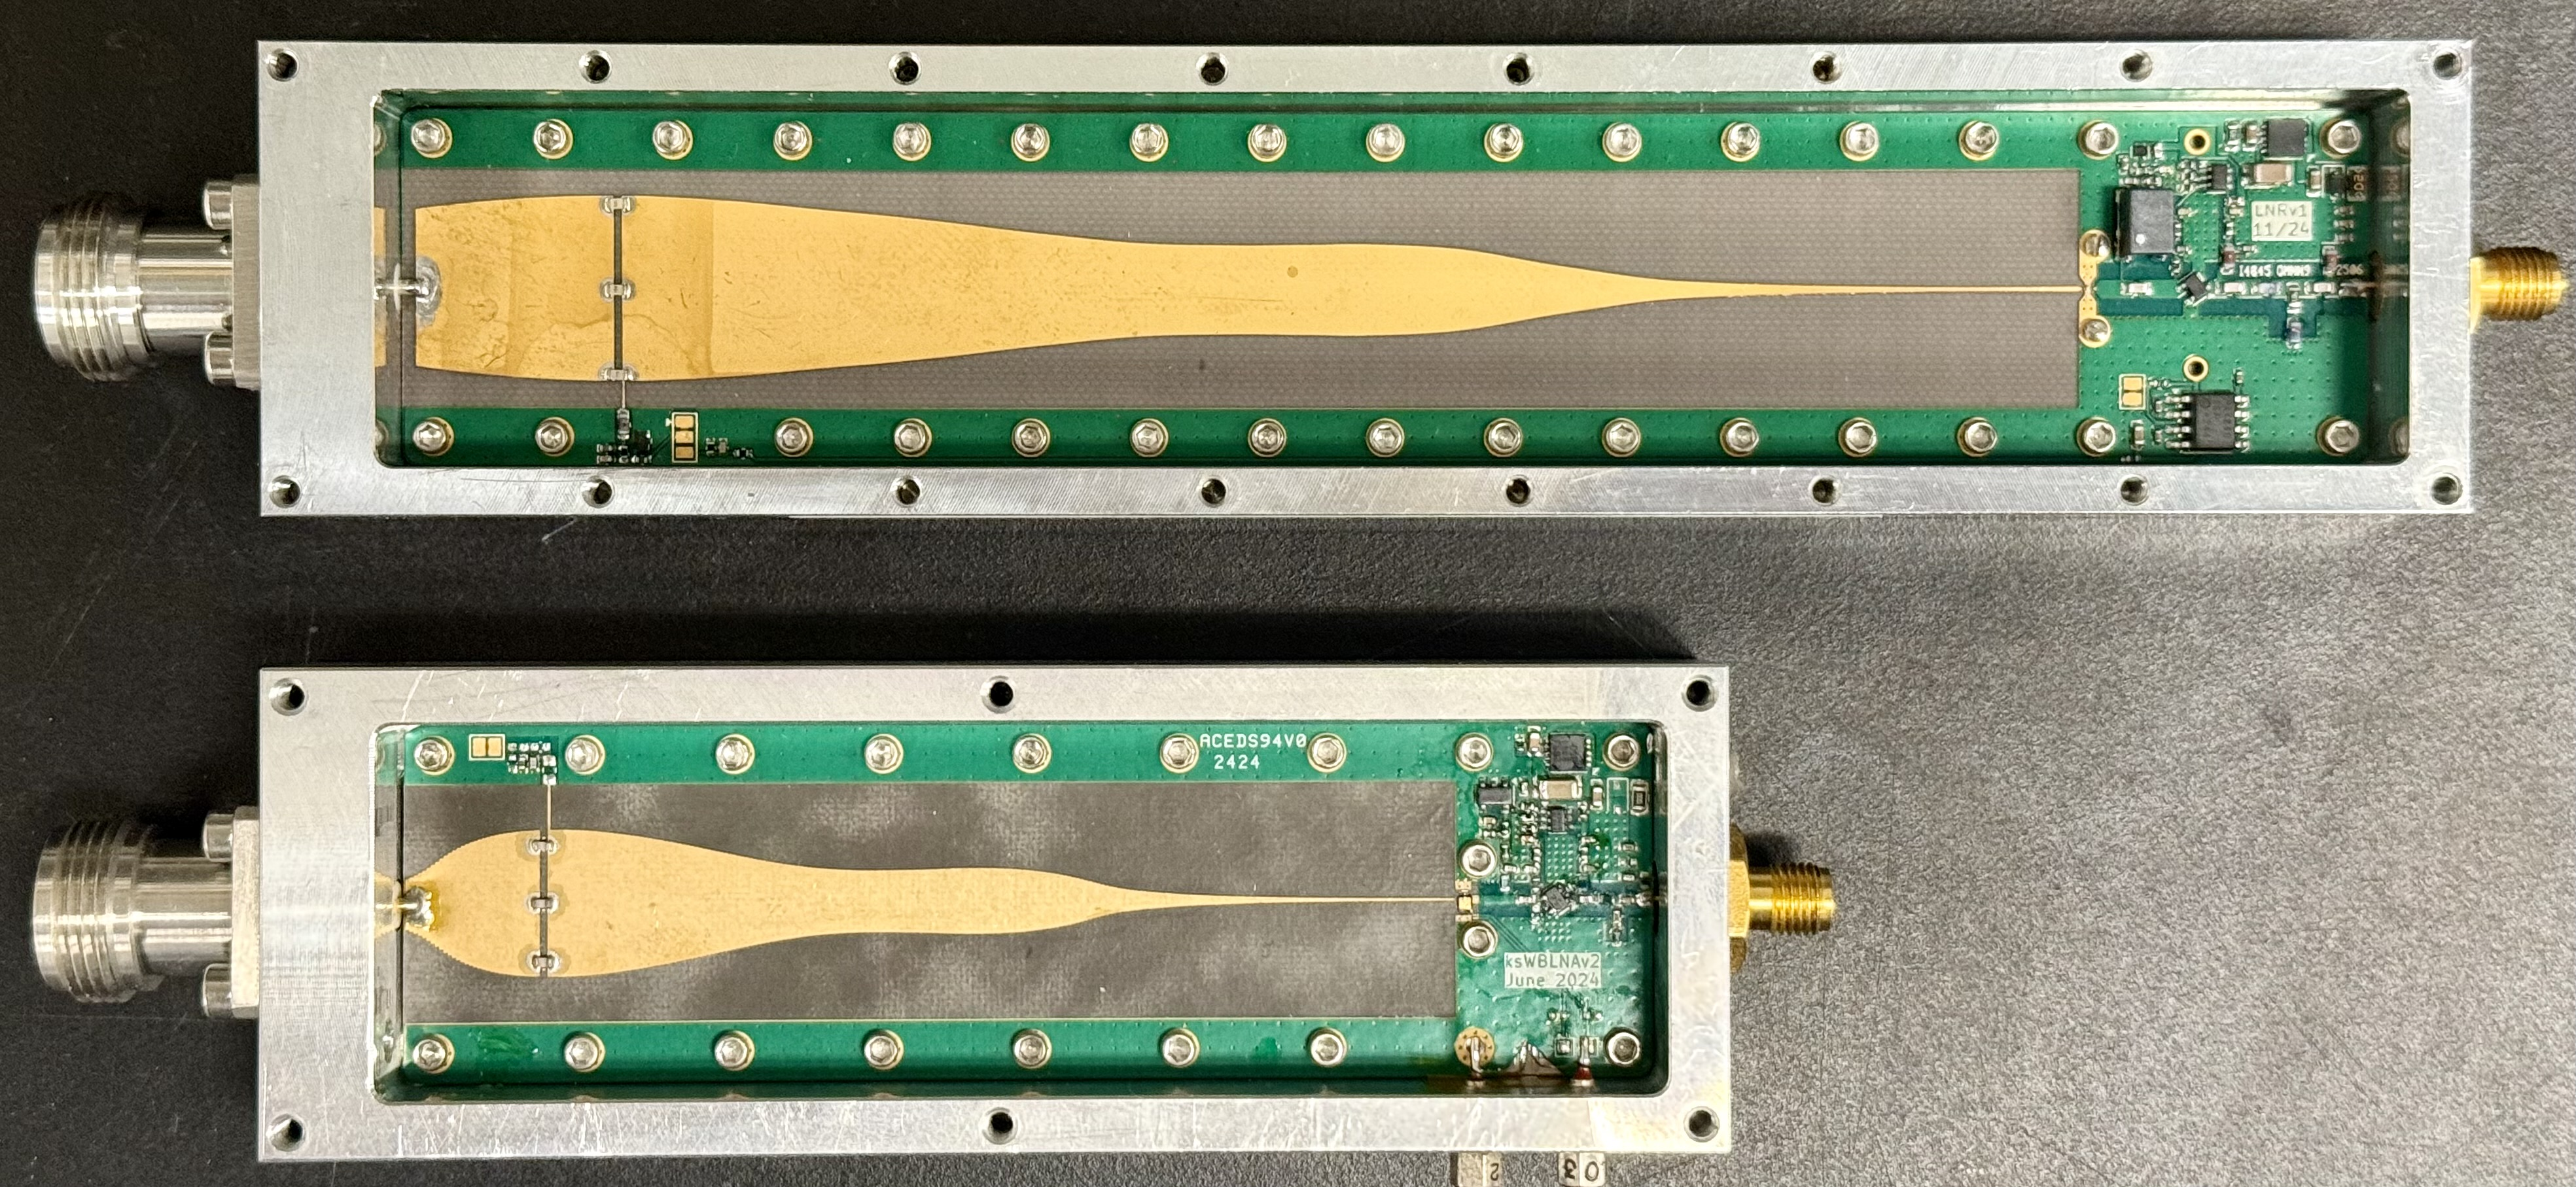
\includegraphics[width=\linewidth]{figures/lnr_v_lna.jpg}
    \caption{Comparison of the co-optimized LNA (in a test chassis) and the previous \qty{50}{\ohm} design}
    \label{fig:lnr_v_lna}
\end{figure}

The results from the optimization were surprising, as the optimal nonuniform line is significantly longer than the previous design.
This seems to indicate a shift in the optimum insertion loss versus noise match space.
At its core, the nonuniform matching approach requires long lines to successfully match complex loads~\cite{xiaoImpedanceMatchingComplex2002}.
As discussed in \autoref{ch:lna}, a well-matched, long line is at odds with the insertion loss of the line itself, implying that there exists some optimum compromise between the length of the line providing a quality noise match and the loss of the line.
When co-optimizing with the DSA-2000 feed, this optimum has shifted to favor longer lines.
In short, the design can tolerate the loss introduced from the longer line, as the noise otherwise introduced due to mismatch at the band edges is so great.

\begin{figure}[ht!]
    \centering
    \includestandalone[mode=buildnew]{figures/lnr_noise}
    \caption{Simulated noise temperature of co-optimized and original LNA designs given a simulated feed source impedance}
    \label{fig:lnr_sim_noise}
\end{figure}

The simulated equivalent noise temperatures for the previous design and the new design are presented in \autoref{fig:lnr_sim_noise}.
Although the difference in mean noise temperature is small (\qty{\approx1}{\K}), the improvement in noise from \qty{700}{\MHz} to \qty{800}{\MHz} is massive.
As survey speed is $\propto\lambda^2$, this improvement in the low frequency performance is huge.
\printbibliography[heading=subbibliography]
\end{refsection}

\chapter{GReX: An instrument overview and new upper limits on the Galactic FRB population} \label{ch:grex}
\publishedas{shilaGReXInstrumentOverviewSubmitted}
\begin{refsection}
\input{grex}
\printbibliography[heading=subbibliography]
\end{refsection}

\appendix

\chapter{Automatic Differentiation} \label{ch:ad_appen}
\begin{refsection}
At its core, AD is the recursive application of the chain rule:
%
\begin{equation}
	\frac{d}{dx}\left[f\left(g\left(x\right)\right)\right] = f^{\prime}\left(g\left(x\right)\right)g^{\prime}\left(x\right)
	\label{eq:chain_rule}
\end{equation}
%
To apply the chain rule to computer programs, we must reinterpret the sequence of instructions that a program performs as function composition.
For a complicated program with many steps, this is equivalent to nested composition $f(g(h(w(...(x)))))$.
For deep nesting, it may be more useful to imagine the flow of values through the program as a computational graph.
For the case of $f(g(x))$, there are three ``primal'' values: $x$, $g(x)$, and $f(g(x))$.
Correspondingly, there are two ``tangent'' values, $g^{\prime}(x)$ and $f^{\prime}(g(x))$.
This graph is shown in \autoref{fig:simple_ast} with square nodes indicating start and stop values, circular nodes indicating computation, and edges showing the flow of values.

\begin{figure}[ht!]
	\centering
	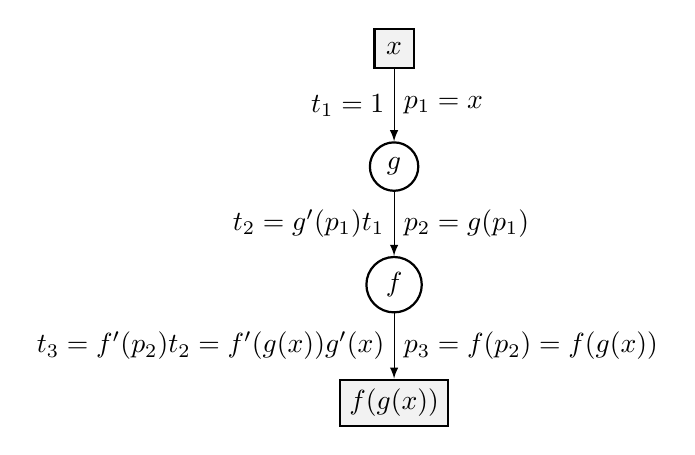
\begin{tikzpicture}[scale=1]
		\node (x) [value] at (0,0) {$x$};
		\node (g) [computation] at (0,-1.5) {$g$};
		\node (f) [computation] at (0,-3) {$f$};
		\node (v) [value] at (0,-4.5) {$f(g(x))$};
		\draw [->] (x) to node[left] {$t_{1}=1$} node[right] {$p_{1}=x$} (g);
		\draw [->] (g) to node[left] {$t_{2}=g^{\prime}(p_{1})t_{1}$} node[right] {$p_{2}=g(p_{1})$} (f);
		\draw [->] (f) to node[left] {$t_{3}=f^{\prime}(p_{2})t_{2}=f^{\prime}(g(x))g^{\prime}(x)$} node[right] {$p_{3}=f(p_{2})=f(g(x))$} (v);
	\end{tikzpicture}
	\caption{Computational graph of forward-mode evaluation of $f(g(x))$ }
	\label{fig:simple_ast}
\end{figure}

The values flowing down the right side of the graph in \autoref{fig:simple_ast} represent the normal evaluation of the program.
The values on the left represent the accumulated tangents, with the initial value ``seeded'' as unity.
Each primal computation relies on the values that immediately precede it.
Similarly, the tangent components rely on the previous tangent and primal component.
At the end of this graph, we have computed both the primal result and the tangent.
This accumulation of tangent values alongside the primal values to build the resulting derivative is known as forward-mode AD.

To extend forward-mode AD to multivariate functions, we set the tangent ``seed'' value of the independent variable of interest to unity, with the remaining variables' tangents set to zero.
Consider this more complicated computer program:
% 
\begin{algorithm}[H]
\caption{Example differentiable program}
\begin{algorithmic}
\STATE 
\STATE {$f$}$(a, b)$:
\STATE \hspace{0.5cm}$x \gets a^2 $
\STATE \hspace{0.5cm}$y \gets \sin{b}$
\STATE \hspace{0.5cm}\textbf{return}  $x*y$
\end{algorithmic}
\end{algorithm}
%
Suppose we want to find $\partial f/\partial b$.
The graph of all operations, primals, and tangents to do so is shown in \autoref{fig:ast}.

\begin{figure}[ht!]
	\centering
	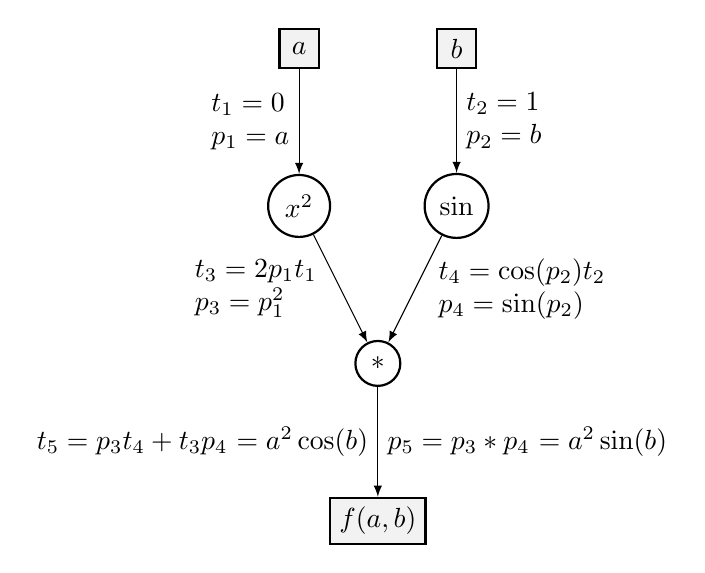
\begin{tikzpicture}[scale=1]
		\node (a) [value] at (0,0) {$a$};
		\node (b) [value] at (2,0) {$b$};
		\node (pow) [computation] at (0,-2) {$x^{2}$};
		\node (sin) [computation] at (2,-2) {$\sin$};
		\draw [->] (a) to node[align=left,left] {$t_{1}=0$\\$p_{1}=a$} (pow);
		\draw [->] (b) to node[align=left,right] {$t_{2}=1$\\$p_{2}=b$}(sin);
		\node (times) [computation] at (1,-4) {$*$};
		\draw [->] (pow) to node[align=left,left,xshift=-5pt] {$t_{3}=2p_{1}t_{1}$ \\ $p_3=p_1^2$} (times);
		\draw [->] (sin) to node[align=left,right,xshift=5pt] {$t_{4}=\cos(p_{2})t_{2}$ \\ $p_{4}=\sin(p_{2})$}(times);
		\node (f) [value] at (1,-6) {$f(a,b)$};
		\draw [->] (times) to node[align=right, left] { $t_{5}=p_{3}t_{4} + t_{3}p_{4}$  $=a^2\cos(b)$}
		node[align=right, right] {$p_{5}=p_{3}*p_{4}$  $=a^2\sin(b)$}(f);
	\end{tikzpicture}
	\caption{Computational graph of forward-mode evaluation of $f(a,b)$, with the tangent seeded on $b$}
	\label{fig:ast}
\end{figure}

To compute $\partial f/\partial a$, we would set $t_{1}$ to unity and $t_{2}$ to zero and perform an additional sweep.
This generalizes to an approach for evaluating gradients for functions of the form $f: \R^{n} \rightarrow \R^{m}$.
Requiring one pass per independent variable implies that gradient evaluation in forward-mode has a complexity of $\mathcal{O}(n)$ for an $n$-dimensional input.
As such, forward-mode performs well for $f: \R \rightarrow \R^{n}$ but has no better complexity than finite-differencing for $f: \R^{n} \rightarrow \R$ (while maintaining machine-precision accuracy).

While forward-mode is simple and is straightforward to implement, the linear complexity poses a problem for high-dimensional functions such as large machine learning models or highly parameterized circuit optimizations.
A solution is to change the manner in which we decompose the chain rule.
Instead of computing the full derivative of each nested function recursively, we compute the derivate \textit{with respect to} each nested function recursively and work backwards.
In practice, this amounts to evaluating the primal trace of the function as before, but now collecting all primal values and their partial derivatives with respect to each parent value.
Then, we seed the ``adjoint'' of the dependent variable (output) with unity and work backwards through the graph, applying the chain rule utilizing the precomputed partials.
This is known as reverse-mode AD.

Looking again at our unary $f: \R \rightarrow \R$ function of $y = f(g(x))$, we draw the computational graph shown in \autoref{fig:reverse_simple_ast}.

\begin{figure}[ht!]
	\centering
	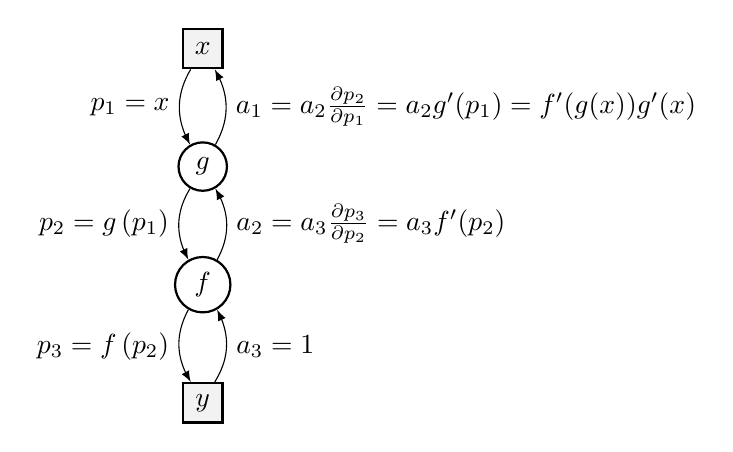
\begin{tikzpicture}[scale=1]
		\node (x) [value] at (0,0) {$x$};
		\node (g) [computation] at (0,-1.5) {$g$};
		\node (f) [computation] at (0,-3) {$f$};
		\node (y) [value] at (0,-4.5) {$y$};
		\draw [->, bend right] (x) to node[left] {$p_{1}=x$} (g);
		\draw [->, bend right] (g) to node[right] {$a_{1}=a_{2}\frac{\partial p_{2}}{\partial p_{1}}=a_{2}g^{\prime}(p_{1})=f^{\prime}(g(x))g^{\prime}(x)$} (x);
		\draw [->, bend right] (g) to node[left] {$p_{2}=g\left(p_{1}\right)$} (f);
		\draw [->, bend right] (f) to node[right] {$a_{2}=a_{3}\frac{\partial p_{3}}{\partial p_{2}}=a_{3}f^{\prime}(p_{2})$} (g);
		\draw [->, bend right] (f) to node[left] {$p_{3}=f\left(p_{2}\right)$} (y);
		\draw [->, bend right] (y) to node[right] {$a_{3}=1$} (f);
	\end{tikzpicture}
	\caption{Graph of reverse-mode evaluation of $f(g(x))$ }
	\label{fig:reverse_simple_ast}
\end{figure}

Here we again see the primal, normal program execution of the function on the left, and then the reverse pass accumulation of the adjoints on the right.
The resulting adjoint, $a_{1}$, is identical to the resulting forward-mode tangent $t_{3}$ from \autoref{fig:simple_ast}.
The difference is that in this case, all the intermediate values and the partial derivatives need to be stored, whereas in forward-mode, each step relies solely on the previous tangent and primal values in the graph.

The procedure becomes more complicated with less trivial, multi-arity functions.
Consider the function example from \autoref{fig:ast}, shown in \autoref{fig:reverse_ast} now in reverse-mode.

\begin{figure}[t]
	\centering
	\subfloat[Forward Sweep] {
		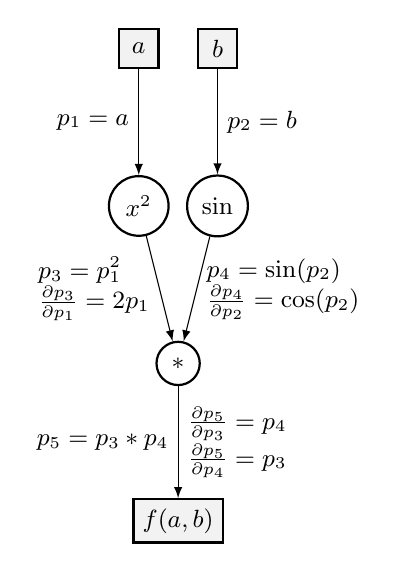
\begin{tikzpicture}[scale=1]
			\tikzstyle{every node}=[font=\small]
			\node (a) [value] at (0.5,0) {$a$};
			\node (b) [value] at (1.5,0) {$b$};
			\node (pow) [computation] at (0.5,-2) {$x^{2}$};
			\node (sin) [computation] at (1.5,-2) {$\sin$};
			\draw [->] (a) to node[align=left,left] {$p_{1}=a$} (pow);
			\draw [->] (b) to node[align=left,right] {$p_{2}=b$}(sin);
			\node (times) [computation] at (1,-4) {$*$};
			\draw [->] (pow) to node[align=left,left,xshift=0pt] {$p_3=p_1^2$ \\
				$\frac{\partial p_{3}}{\partial p_{1}} = 2p_{1}$
			} (times);
			\draw [->] (sin) to node[align=left,right,xshift=0pt,yshift=0pt] {$p_{4}=\sin(p_{2})$ \\
				$\frac{\partial p_{4}}{\partial p_{2}}=\cos(p_{2})$
			}(times);
			\node (f) [value] at (1,-6) {$f(a,b)$};
			\draw [->] (times) to node[left] {$p_{5}=p_{3}*p_{4}$}
			node[align=left,right] {$\frac{\partial p_{5}}{\partial p_{3}} = p_{4}$ \\ $\frac{\partial p_{5}}{\partial p_{4}} = p_{3}$}
			(f);
		\end{tikzpicture}
	}
    \quad
	\subfloat[Reverse Sweep] {
		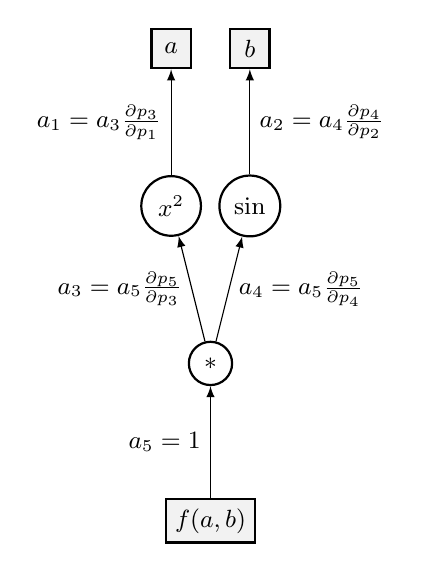
\begin{tikzpicture}[scale=1]
			\tikzstyle{every node}=[font=\small]
			\node (a) [value] at (0.5,0) {$a$};
			\node (b) [value] at (1.5,0) {$b$};
			\node (pow) [computation] at (0.5,-2) {$x^{2}$};
			\node (sin) [computation] at (1.5,-2) {$\sin$};
			\draw [->] (pow) to node[align=left,left] {$a_{1}=a_{3}\frac{\partial p_{3}}{\partial p_{1}}$} (a);
			\draw [->] (sin) to node[align=left,right, xshift=0pt] {$a_{2}=a_{4}\frac{\partial p_{4}}{\partial p_{2}}$}(b);
			\node (times) [computation] at (1,-4) {$*$};
			\draw [->] (times) to node[align=left,left,xshift=0pt] {$a_{3} = a_{5}\frac{\partial p_{5}}{\partial p_{3}}$} (pow);
			\draw [->] (times) to node[align=left,right,xshift=0pt] {$a_{4}=a_{5}\frac{\partial p_{5}}{\partial p_{4}}$} (sin);
			\node (f) [value] at (1,-6) {$f(a,b)$};
			\draw [->] (f) to node[left] {$a_{5}=1$} (times);
		\end{tikzpicture}
	}
	\caption{Graph of reverse-mode evaluation of $f(a,b)$ }
	\label{fig:reverse_ast}
\end{figure}

Again, in the forward sweep, we collect primal values as well as partial derivates.
Then, in the reverse-mode, we collect adjoints down every branch by multiplying the previous adjoint by the appropriate precomputed  partial derivates.
This offers several advantages, the first of which is that in one pass, we have computed the full gradient.
Additionally, we have done so with fewer operations than in the forward-mode.
Often, this is a more efficient way of computing the gradient.
However, the reverse sweep requires us to build the computation graph in memory and store intermediate values and partials, while forward-mode only requires the previous tangents and primals.
This is a classic example of a memory-time complexity tradeoff.
In general, for functions of the form $f: \R^{n} \rightarrow \R^{m}$ where $m \gg n$, forward-mode is preferred.
However, for general optimization problems, reverse-mode is typically higher performance, as it solves $f: \R^{n} \rightarrow \R$ for a scalar cost function.
Benchmarking to choose the right approach is required when the input and output dimensions have similar orders of magnitude.

Efficient implementations of these algorithms have become commonplace due to their usage in training large machine learning models.
For a more in-depth discussion on the field of AD and implementation details, see~\cite{baydinAutomaticDifferentiationMachine2017}.
\printbibliography[heading=subbibliography]
\end{refsection}

\chapter{Useful Results} \label{ch:eqns}
\begin{refsection}
\section{Interferometer Survey Speed and Sensitivity} \label{sec:survey_speed}

To derive the survey speed of a radio interferometer, we start with the radiometer equation:
\begin{equation}
    \sigma_T = \frac{T_\text{Sys}}{\sqrt{\Delta\nu\tau}}
\end{equation}
For system noise temperature $T_\text{Sys}$, bandwidth $\Delta\nu$, and integration time $\tau$, we can compute the RMS error (in Kelvin).
If we want to know the signal-to-noise ratio for an observation of a point source, we can define the ratio of the source's induced antenna temperature $T_a$ over this RMS noise level
\begin{equation}
    \text{SNR} = \frac{T_a}{\sigma_T} = \frac{T_a}{T_\text{Sys}}\sqrt{\Delta\nu\tau}
    \label{eq:radiometer_snr}
\end{equation}
Sources in the sky vary wildly in flux density, so to come up with a single metric, we can pick some arbitrary, minimum source flux density to set our SNR, $S_\nu$.
This point source flux density induces an antenna temperature via
\begin{equation}
    T_a = \frac{S_\nu A_e}{2k_B}
\end{equation}
where $A_e$ is the effective collecting area of the array and $k_B$ is Boltzmann's constant.
For reflector-based antennas, the effective aperture is equal to the reflector's physical area, scaled by some aperture efficiency, $\eta_a$, typically in the \num{0.7}-range.
We then multiply this by $N$ antennas to get the total effective collecting area for the entire array.
\begin{equation}
    A_e = \frac{N\eta_a\pi D^2}{4}
\end{equation}
Now, we can find the integration time required to achieve an SNR of unity.
\begin{equation}
    \tau = \frac{1}{\Delta\nu}\left[\frac{8k_B T_\text{Sys}}{S_\nu N\eta_a\pi D^2}\right]^2
    \label{eq:integration_time}
\end{equation}
As this is the time required to survey one portion of the sky, the last missing piece is how much of the sky we surveyed in this pointing.
Again, for reflectors, we could use the full-width half-maximum in steradians, or the beam solid angle, $\Omega_B$.
For high-gain reflectors (as are used in radio astronomy), these are almost identical.
For any antenna, the beam solid angle is defined as
\begin{equation}
    \Omega_B = \frac{\lambda^2}{A_e^\prime}
\end{equation}
where $A_e^\prime$ here is the effective aperture (of the primary beam, not the total array).
So, we can write
\begin{equation}
    \Omega_B = \frac{4\lambda^2}{\pi\eta_aD^2}
\end{equation}
Finally, we can define survey speed as the time required to survey a given beam solid angle to some fixed minimum point source flux density as
\begin{equation}
    \text{SS}~\text{(sr/s)} = \frac{\Omega_B}{\tau} = \eta_a\pi\Delta_\nu\left[\frac{\lambda S_\nu N D}{4k_B T_\text{Sys}}\right]^2
\end{equation}
If we take $S_\nu$ to be in Jy (\qty{1e-26}{\W/\Hz/\m^2}) and convert to deg$^2$ per hour, we can approximate this as
\begin{equation}
        \text{SS}~(\text{deg}^2/\text{hr}) \approx 1.217\eta_a\Delta_\nu\left[\frac{\lambda S_\nu N D}{T_\text{Sys}}\right]^2
\end{equation}
The important implications of this relation are the quadratic terms in $\lambda$, $N$, $D$, and $T_\text{Sys}$, as these are all design parameters.

In addition to survey speed, we can recast \autoref{eq:radiometer_snr} as a sensitivity metric.
In other words, we can find what flux density ($S_\nu$) we can measure at a $1\sigma_T$-level in some fixed integration time $\tau$.
\begin{equation}
    S_\nu~(\text{W}/\text{m}^2/\text{Hz}) = \frac{8k_BT_\text{Sys}}{\pi\eta_aD^2N\sqrt{\Delta_\nu\tau}}
\end{equation}
We can again simply this if we assume $\tau$ is one hour, our answer is in $\mu$Jy (\qty{1e-32}{\W/\Hz/\m^2}), and $\Delta_\nu$ is in GHz, we can write
\begin{equation}
    S_\nu~(\mu\text{Jy @ 1 hr}) \approx 1852\frac{T_\text{Sys}}{\eta_aD^2N\sqrt{\Delta_{\nu\text{(GHz)}}}}
\end{equation}

If we use some typical DSA-2000 numbers of $\Delta_\nu=$ \qty{1.3}{\GHz}, $D=$ \qty{5}{\m}, $N=$ \num{2000}, $\eta_a=$ \num{0.7}, $T_\text{Sys}=$ \qty{25}{\K}, at a center wavelength $\lambda$ of \qty{22}{\cm}, we find:
\begin{align}
    \text{SS}~(\text{deg}^2/\text{hr @ 2}\mu\text{Jy}) &= 31.3 \\
    S_\nu~(\mu\text{Jy @ 1 Hr}) &= 1.16
\end{align}

\section{Intermodulation Products} \label{sec:intermod}
Given a voltage transfer function of some nonlinear RF component
\begin{equation}
    v_\text{Out} = f(v_\text{In})
\end{equation}
we can find the Taylor (Maclaurin) series expansion of the nonlinear $f$ to give us
\begin{equation}
    v_\text{Out} = \sum_{n=0}^{\infty}\frac{f^{(n)}(0)}{n!}v_\text{In}^n = a_0 + a_1v_\text{In} + a_2v_\text{In}^2 + a_3v_\text{In}^3 \dots
    \label{eq:intermod_expansion}
\end{equation}
where the coefficients $a_0$, $a_1$, etc. are proportional to the $n$-th derivative of $f$.
Consider an input $v_\text{In}$ composed of a sum of two tones close in frequency:
\begin{equation}
    v_\text{In} = V_0(\cos{\omega_1t} + \cos{\omega_2t)}
\end{equation}
Plugging this into \autoref{eq:intermod_expansion}, we find
\begin{align}
    v_\text{Out} = a_0 &+ a_1V_0(\cos{\omega_1t} + \cos{\omega_2t)} \\ &+ a_2V_0^2(\cos{\omega_1t} + \cos{\omega_2t)}^2 \\&+ a_3V_0^3(\cos{\omega_1t} + \cos{\omega_2t)}^3 \dots
\end{align}
Using trigonometric identities, we can expand this to
\begin{align}
v_\text{Out} = a_0 &+ a_1V_0(\cos{\omega_1t + \cos{\omega_2t)}} \notag\\
    &+ \frac{a_2V_0^2}{2}(2\cos{(\omega_1+\omega_2)t} + 2\cos{(\omega_1-\omega_2)t}) \notag\\
    &+ \frac{a_2V_0^2}{2}(\cos{2\omega_1t} + \cos{2\omega_2t}  +1 ) \notag\\
    &+ \frac{a_3V_0^3}{4}(
    \cos{3\omega_1t} + 
    \cos{3\omega_2t} + 
    9\cos{\omega_1t} +
    9\cos{\omega_2t}
    ) \notag\\
    &+
    \frac{a_3V_0^3}{4}(
    3\cos{(\omega_1-2\omega_2)t} + 
    3\cos{(2\omega_1-\omega_2)t}) \notag\\
    &+ \frac{a_3V_0^3}{4}(
    3\cos{(\omega_1+2\omega_2)t} +
    3\cos{(2\omega_1+\omega_2)t}) \dots
\end{align}
Here, we can see that increasing powers from the series expansion leads to sum and difference frequencies of the form $n\omega_1 \pm m\omega_2$ for positive integers $m$ and $n$.
As the input voltage in the two tones increases, so do these so called ``intermodulation'' products.
If the input power is small, these products will be well beneath the noise floor.
However, as the power increases, the output power of the fundamental ($\cos{\omega_n t}$ increases linearly while the power in the intermodulation powers grow with the input voltage squared for the second-order terms and with the cube for the third-order terms.
If the amplifier did not saturate, eventually the power of these tones at the output would intersect.
The hypothetical power at which these intermodulation tones intersect are the $n$-th order intercept points.

\subsection{2nd Order Distortion}
The total power delivered at either fundamental into a \qty{1}{\ohm} load is
\begin{equation}
    P_{\omega_{1}} = \frac{1}{2}a_1^2V_0^2
\end{equation}
recalling that these voltage phasors are defined with peak magnitudes, and so power is defined as $1/2Re\{VI^*\}$.
The total power delivered at one of the 2nd order mixing terms ($\cos{\omega_1\pm\omega_2}$) is
\begin{equation}
    P_{\omega_1+\omega_2} = \frac{1}{2}a_2^2V_0^4
\end{equation}
The definition of the intercept point is when the powers at the fundamental and the intermodulation product are equal.
\begin{equation}
    \frac{1}{2}a_1^2V_{IP2}^2 = \frac{1}{2}a_2^2V_{IP2}^4
\end{equation}
Solving for $V_{IP2}$ yields
\begin{equation}
    V_{IP2} = \frac{a_1}{a_2}
\end{equation}
We define the output intercept point as the power at the fundamental which leads to this intersection
\begin{equation}
    \text{OIP2} = P_{\omega_1}|_{V_0=V_{IP2}} = \frac{1}{2}a_1^2V_{IP2}^2 = \frac{a_1^4}{2a_2^2}
\end{equation}
Finally, we can find that the power of the output intermodulation product can be rewritten in terms of the power of the fundamental and OIP2
\begin{equation}
    P_{\omega_1+\omega_2} = \frac{1}{2}a_2^2V_0^4 = \frac{\left(\frac{1}{2}a_1^2V_0^2\right)^2}{a_1^4(2a_2^2)^{-1}} = \frac{P_{\omega_{1}}^2}{\text{OIP2}}
    \label{eq:2nd_order_oip2_powers}
\end{equation}
or
\begin{align}
    \text{OIP2}~(W) &= \frac{P_{\omega_{1}}^2}{P_{\omega_1+\omega_2}} \\
    \text{OIP2}~(\text{dBm}) &= 2P_{\omega_{1}} - P_{\omega_1+\omega_2}
\end{align}

\subsection{Cascaded Distortion}
Shown in figure \fixme{fixme}, given two components with power gains $G_1$ and $G_2$ with output nth-order output intercept points $\text{OIP}n^\prime$ and $\text{OIP}n^{\prime\prime}$, we want to find the effect of combining their distortions.
As the tones are deterministic, the phase of the various intermodulation product impact the output.
As such, we need to work out the cascade in voltages.

Using the result from \autoref{eq:2nd_order_oip2_powers}, we can compute the output voltage of the 2nd order term as
\begin{equation}
    V_{\omega_1+\omega_2}^\prime = \sqrt{P_{\omega_1+\omega_2}^\prime Z_0} = P_{\omega_{1}}^\prime\sqrt{\frac{Z_0}{\text{OIP2}^\prime}}
\end{equation}
As the phase of these voltages is unknown, we can assume the worst-case of the distortion products adding in-phase.
Therefore, the total 2nd-order distortion voltage at the output of the second component is
\begin{equation}
    V_{\omega_1+\omega_2}^{\prime \prime} = P_{\omega_{1}}^\prime\sqrt{\frac{G_2Z_0}{\text{OIP2}^\prime}} + P_{\omega_{1}}^{\prime \prime}\sqrt{\frac{Z_0}{\text{OIP2}^{\prime \prime}}}
\end{equation}
As $P_{\omega_{1}}^{\prime \prime}=G_2P_{\omega_{1}}^{\prime}$, we have
\begin{align}
    V_{\omega_1+\omega_2}^{\prime \prime} &= \left(
    \frac{\sqrt{G_2}}{G_2\sqrt{\text{OIP2}^\prime}} + \frac{1}{\sqrt{\text{OIP2}^{\prime \prime}}}
    \right)P_{\omega_{1}}^{\prime \prime}\sqrt{Z_0} \notag\\
    & =
    \left(
    \frac{1}{\sqrt{G_2\text{OIP2}^\prime}} + \frac{1}{\sqrt{\text{OIP2}^{\prime \prime}}}
    \right)P_{\omega_{1}}^{\prime \prime}\sqrt{Z_0}
\end{align}
The total output distortion power is
\begin{equation}
    P_{\omega_1+\omega_2}^{\prime \prime} = \frac{\left(V_{\omega_1+\omega_2}^{\prime \prime}\right)^2}{Z_0}
    =    \left(
    \frac{1}{\sqrt{G_2\text{OIP2}^\prime}} + \frac{1}{\sqrt{\text{OIP2}^{\prime \prime}}}
    \right)^2(P_{\omega_{1}}^{\prime \prime})^2
    = \frac{(P_{\omega_{1}}^{\prime \prime})^2}{\text{OIP2}}
\end{equation}
Therefore the 2nd order intercept of the cascaded system with coherent products is
\begin{equation}
    \text{OIP2} = \left(
    \frac{1}{\sqrt{G_2\text{OIP2}^\prime}} + \frac{1}{\sqrt{\text{OIP2}^{\prime \prime}}}
    \right)^{-2}
\end{equation}
Although the worst case is useful for putting a bound on the distortion, in practical systems with many components, the phases between various stages may be randomly distributed.
In that case, we can treat the contributions as incoherent and directly sum the powers of the intermodulation products.
\begin{equation}
    P_{\omega_1+\omega_2}^{\prime \prime} = G_2\frac{(P_{\omega_1}^{\prime})^2}{\text{OIP2}^{\prime}}+ \frac{(P_{\omega_1}^{\prime \prime})^2}{\text{OIP2}^{\prime \prime}} = \left(
    \frac{1}{G_2\text{OIP2}^{\prime}} + \frac{1}{\text{OIP2}^{\prime \prime}}
    \right)(P_{\omega_1}^{\prime \prime})^2
\end{equation}
Again solving for the total cascaded 2nd order intercept, incoherently combined
\begin{equation}
    \text{OIP2} = \left(
    \frac{1}{G_2\text{OIP2}^{\prime}} + \frac{1}{\text{OIP2}^{\prime \prime}}
    \right)^{-1}
\end{equation}

The derivations for the 3rd order intercept can be found in~\cite{pozarMicrowaveEngineering2012}.
\printbibliography[heading=subbibliography]
\end{refsection}

\chapter{GReX Errata}
\begin{refsection}
\section{Telescope Calibration}\label{sec:Acalibration}
The factors of importance for determining the instrument sensitivity are three-fold: (1) the telescope response to an incoming signal as a function of angle, (2) the gain of the receiver, and (3) the system temperature of the instrument. 
Noise is added to an incoming signal during its propagation through the amplifiers and other electronics of the system. 
It is practical to begin by considering the specific intensity ($I_\nu$) of a signal, since it is a conserved quantity through empty space. 
However, the quantity that describes the spectral power of the source received at the detector is the flux density,
\begin{equation}
    S_\nu=\int_\Omega d\Omega\left[I_\nu(\theta,\phi)B(\theta)\cos\theta\right].\label{eq:flux_density}
\end{equation}
$B(\theta)$ describes the response of the receiver to incoming radiation and is equivalent to the normalized effective area $A_{e}(\theta)/A_0$, where $A_0=A_e(\theta=0)=A_{e,max}$. 
In this notation, $\theta=0$ points along the normal vector of the telescope receiver and $\phi$ describes the azimuthal angle about that normal vector.
The $\cos\theta$ term in the integral describes the effect of projecting the incoming spectral power across the detector at different inclination angles. 
The beam size of a telescope is relatively small in most cases, so $B(\theta)$ falls to zero rapidly and $\cos\theta\approx1$, but this approximation does not hold for the GReX instrument. 
Since the behavior of the $\cos\theta$ term describes the Flux Density seen at the detector, it is absorbed into the beam response function $B(\theta)$.
It is standard practice to express the specific intensity ($I_\nu$) of astrophysical signals in terms of their equivalent brightness temperature ($T_b$) using the Raleigh-Jeans approximation:
\begin{equation}
    I_\nu \approx \frac{2k_B T_b}{\lambda^2}. \label{eq:RJ}
\end{equation}
For a given distribution of brightness temperature on the sky ($T_b(\theta,\phi)$), the detected flux density is 
\begin{equation}
    S_\nu=\frac{2k_B}{\lambda^2}\int_\Omega d\Omega\left[T_b(\theta,\phi)B(\theta)\right].\label{eq:FDT}
\end{equation}
We can prescribe a constant effective temperature ($T_{eff}$) that gives the same flux density as for an arbitrary brightness distribution:
\begin{equation*}
    \int_\Omega d\Omega\left[T_b(\theta,\phi)B(\theta)\right]=T_{eff}\int_\Omega d\Omega\left[B(\theta)\right]=T_{eff}\Omega_B.
\end{equation*}
For a single-pixel instrument like GReX, this is equivalent to the antenna temperature contributed by the source. 
If the source does have a constant brightness temperature across the beam, then it is apparent that $T_{eff}$ accurately describes the source temperature. 
However, for sources covering a small patch of sky ($T_b(\theta,\phi)=T_b\Delta^\prime$, where$\Delta^\prime\sim\delta(\theta-\theta^\prime, \phi-\phi^\prime)$) centered at $(\theta^\prime,\phi^\prime)$ and with total solid angle $\Omega_\Delta$, the beam response and source brightness temperature are approximately constant and
\begin{equation*}
    T_{eff}\approx\frac{\int_\Omega T_b(\theta,\phi)B(\theta)\Delta^\prime d\Omega}{\Omega_B} =T_b B(\theta^\prime)\frac{\Omega_\Delta}{\Omega_B}.
\end{equation*}
Since the flux density is related to the effective temperature like
\begin{equation*}
    S_\nu=\frac{2k_B\Omega_B}{\lambda^2}T_{eff},
\end{equation*}
a source at a distance $\delta\theta$ from the center of the beam will have its flux density at the receiver reduced by a factor $B(\delta\theta)$ than if it were centered in the beam:
\begin{equation*}
    S_\nu(\delta\theta) \approx B(\delta\theta)S_\nu(0). \label{eq:FnuAstro}
\end{equation*}
While flux density is usually not used to describe extended sources with variable brightness temperature, we do use it for calibration of the instrument as described in \autoref{sec:beam_model} with measured and simulated values of the hydrogen I line brightness temperature from diffuse Galactic gas. 
As such, we include an expression for the antenna temperature for a well-known brightness distribution:
\begin{equation}
    T_{A}=\int_\Omega d\Omega \left[T_b(\theta,\phi)\hat{B}(\theta)\right],\label{eq:Teff}
\end{equation}
where $\hat{B}$ describes the normalized telescope response,
\begin{equation}
    \hat{B}(\theta)=\frac{B(\theta)}{\Omega_B}.\label{eq:Bnorm}
\end{equation}
The effective area of the telescope has the intrinsic property that
\begin{equation*}
\langle A_e\rangle_\Omega=\frac{\int_\Omega}{4\pi}=\frac{\lambda^2}{4\pi}.
\end{equation*}
Following from this, and $B(\theta)=A_e(\theta)/A_0$,
the maximum effective area is 
\begin{equation}
    A_0=\frac{\lambda^2}{\Omega_B}.\label{eq:Ae}
\end{equation}
The forward gain ($g_f$) relates the antenna temperature to the source flux density as
\begin{equation*}
S_\nu=g_f T_{eff} \to g_f=\frac{2k_B\Omega}{\lambda^2},\label{eq:FDFG}
\end{equation*}
equivalent with
\begin{equation}
    g_f=\frac{2k_B}{A_0}\label{eq:FG}
\end{equation}
Since the forward gain relates the observed temperature of a source by the instrument to the flux density of that source, it is a critical component for defining the sensitivity of the instrument. 

Due to the prevalence of describing observed signals in terms of $T_{A}$, it is convenient to describe all sources that contribute additive power to the signal within the system as a system temperature ($T_{sys}$), even though the noise is not necessarily thermal in nature. 
While there are many sources that contribute to $T_{sys}$, we focus on the thermal noise within the receiver electronics ($T_{rec}$) and the background temperature of the sky ($T_{sky}$). 
At any time, the total observed temperature by the system is
\begin{equation}
    T_{obs}=T_{eff}+T_{sys}=T_{eff}+T_{rec}+T_{sky}.
\end{equation}
However, GReX data is natively stored as linear intensities with arbitrary units ($I_{arb}$). 
The receiver gain ($G$, in $K/arb$) converts the linear intensities into Kelvin,
\begin{equation}
    T_{obs}=GI_{arb}.
\end{equation}
Since $T_{sky}$ is well characterized to account for atmospheric effects and background radiation, our sensitivity analysis needs to account for $G$ and $T_{sys}$ so that the effective source temperature can be isolated as
\begin{equation}
    T_{eff}=GI_{arb}-T_{sky}-T_{rec}.
\end{equation}
We determine $G$ and $T_{sys}$ by performing a Y-factor test with two known values for $T_{sky}$.
We first take measurements of the unobscured sky with a GReX terminal before collecting data again, this time with a slab of room-temperature radio-absorbent foam covering the receiver. 
Under the assumption that there are no significant astrophysical sources present in the data, we now have 
\begin{equation}
    I_1=\frac{T_{sky}+T_{rec}}{G},\\
    I_2=\frac{T_{hot}+T_{rec}}{G}.
\end{equation}
The Y-factor ($Y=I_2/I_1$) is then expanded according to the above equations and rearranged to give the following expression for the receiver temperature,
\begin{equation}
    T_{rec}=\frac{T_{hot}-YT_{sky}}{Y-1}.\label{eq:Trec}
\end{equation}
From this value, the receiver gain is trivially
\begin{equation}
    G=\frac{T_{hot}+T_{rec}}{I_2}=\frac{(T_{hot}-T_{sky})}{(I_2-I_1)}.\label{eq:gain}
\end{equation}
Ideally, this receiver gain is roughly constant over observing epochs, but changes in temperature and degradation of the electronics can cause slow changes in this value. 
Of course, any changes to the programmable gain in the FEM of a GReX terminal will require remeasuring the receiver gain. 
The more volatile value is the system temperature, which can change depending on environmental effect such as prevalence of RFI and accumulation of water in the feed, among other potential issues. 
As such, it is useful to measure $T_{sys}$ semi-regularly. 

Once $G$ and $T_{sys}$ are well characterized for the terminal, we compare the measured $T_{eff}$ of a source to its known flux density to determine the forward gain. 
We utilize all-sky maps of neutral galactic hydrogen to simulate the expected flux density as seen by the GReX terminal and compare this with the measured $T_{eff}$ of the HI line by the instrument to calibrate $g_f$ in \autoref{sec:beam_model}.
The conversion of temperature units into flux densities is commonly applied to the system temperature of an instrument to define its system equivalent flux density (SEFD),
\begin{equation}
    \text{SEFD}=S_{\nu,sys}=g_fT_{sys}.\label{eq:sefd}
\end{equation}
Since we are dealing with dynamic spectra that contain signals across multiple frequency channels, time samples, and polarizations, it is helpful to consider the power and temperature within the detector noise that limits the detectability of a signal. 
A signal spanning a bandwidth $\Delta\nu$ with total integration time $\tau$ that is seen in both polarizations of a dipole antenna will be present in $N=2\Delta\nu\tau$ total samples. 
The detectability of such a signal depends on the signal-to-noise ratio
\begin{equation}
    \text{SNR}=\frac{T_{src}}{T_{rms}},
\end{equation}
where $T_{rms}=\sigma_T/\sqrt{N}$ describes the root-mean-squared noise in the system temperature. 
Assuming that the thermal noise contributing to $T_{sys}$ is exponentially distributed such that $T_{sys}=\mu_T=\sigma_T$, then 
\begin{equation*}
T_{rms}=\frac{T_{sys}}{\sqrt{N}}.
\end{equation*}
We can then rewrite the signal-to-noise ratio as
\begin{equation*}
    \text{SNR}=\frac{T_{src}}{T_{sys}}\sqrt{N}
\end{equation*}
The SNR is a useful measure since this ratio of temperatures is equivalent to the corresponding ratios of native system intensity units and the ratios of Flux Density. 
Converting the above expression to flux densities gives
\begin{equation*}
    S_{\nu,src}=\text{SNR}\frac{\text{SEFD}}{\sqrt{N}}.
\end{equation*}
The flux density threshold for detection is then given by
\begin{equation*}
    S_{\nu,min}=\text{SNR}_{min}\cdot\text{NEFD},
\end{equation*}
where the NEFD (noise-equivalent flux density) is $\text{NEFD}=g_fT_{rms}=\text{SEFD}/{\sqrt{N}}$.

\section{HI Line Simulation}\label{sec:Asimulation}
The LAB data is an all-sky map of the brightness temperatures of neutral galactic hydrogen binned into discrete velocity channels. 
These scalar velocities represent the component of the motion of the neutral galactic hydrogen along the line of sight from the solar system to the gas within the local standard of rest (LSR) frame.
The original data format for the LAB survey had a velocity channel spacing of $\sim 1.031\text{ km/s}$ and a total velocity range of $-450\text{ km/s}$ to $+450\text{ km/s}$, but this data was conglomerated into wider bins with a spacing of $10\text{ km/s}$. 
This was done by averaging the brightness temperatures of the narrower bins into those respective larger bins.
Thus, the LAB all-sky map is stored in \textit{HEALPix}~\cite{gorskiHEALPixFrameworkHighResolution2005} file format with separate files for the difference wide velocity channels. 
Each \textit{HEALPix} velocity-channel file has data stored in two fields: the first is a \textit{TEMPERATURE} field, which gives the brightness temperature within the channel for each sky position pixel; the second is called the \textit{SIMULATION} field, which gives the number of original $\sim 1.031\text{ km/s}$ velocity channels that were used in calculating that brightness temperature. 
From the \textit{TEMPERATURE} field, we construct a map of brightness temperature, $T_{HI}(\ell_j, b_j,v_k)$, where $(\ell_j, b_j)$ describes the central position of the $j^{th}$ pixel in galactic coordinates and $v_k$ gives the $k^{th}$ velocity channel in the LSR frame. 
To construct an expected spectrum of HI from this map for a specific terminal and observing time, we need to: (1) account for the velocity, $\vec{v}_{obs}$, and central pointing, $(\ell,b)_{obs}$, of the terminal in the LSR frame at that time; (2) remove the velocity of the observer in LSR along the LoS to each pixel from the neutral hydrogen velocity in LSR to get the gas velocity in the terminal's frame; (3) compute the angular deviation ($\delta\theta)$ of each pixel from the central pointing of the terminal feed and use that to construct a simulated 2D Gaussian beam response $B(\delta\theta)$; (4) convert hydrogen velocity in the observer frame to HI line frequency ($f_{HI,0}=1420.40575\text{ MHz}$) and bin frequencies into observing channels; and (5) for each frequency channel, integrate the brightness temperature map over the $4\pi$ steradians of sky modulated by the telescope beam response function $(B(\delta\theta,f))$ to get the expected spectrum of brightness temperature of HI as seen from a GReX unit.

To compute the velocity of neutral hydrogen in the reference frame of the GReX terminal along the LoS to each LAB data pixel, we need to start with an expression for the overall gas velocity in the observer frame:
\begin{equation*}
    \vec{v}_H,obs(t) = \vec{v}_{H, LSR} - \vec{v}_{obs, LSR}(t).
\end{equation*}
Then, the velocity of gas along the LoS to the $j^{th}$ data pixel is
\begin{equation*}
    v_{H,obs,j}(t) = \hat{n}_j \cdot (\vec{v}_{H, LSR} - \vec{v}_{obs, LSR}(t)),
\end{equation*}
where $\hat{n}_j$ is the unit vector pointing along that LoS.
The scalar velocity channels of the LAB data are already the gas velocity along the LoS, so our final expression is
\begin{equation*}
    v_{H,j,k,obs}(t) = v_{H,k,LSR} - v_{obs,j,LSR}(t),
\end{equation*}
where $v_{obs,j,LSR}(t)=\hat{n}_j\cdot\vec{v}_{obs, LSR}(t)$ is the component of observer velocity along the $j^{th}$ LoS.
\textit{Astropy} handles the conversion of sky positions and velocities between different reference frames and coordinate systems to generate values for $v_{obs,j,LSR}$. 
We begin by defining an \textit{EarthLocation} object for the terminal in geodetic coordinates ($x_{obs,geo}(\text{lat},\text{lon})$), converting to a location in the barycentric celestial reference system at a specific time ($t$), which is then transformed directly into ICRS and then LSR coordinates ($x_{obs,LSR}(x_{obs,geo},t)$). 
\textit{Astropy} then computes the Cartesian differential of the \textit{EarthLocation} object to determine the the GReX terminal velocity within the LSR frame ($\vec{v}_{obs,LSR}(t)$) in (x,y,z) coordinates. 
The LoS unit vector $\hat{n}_j=\hat{n}(\ell_j,b_j)$ that points from the observer towards the galactic coordinates $\ell_j$ and $b_j$ is generated by converting an \textit{Astropy} \textit{SkyCoord} object at those galactic coordinates into (x,y,z) to remain consistent with $x_{obs,LSR}$ and $\vec{v}_{obs,LSR}(t)$. 
The terminal's velocity within the LSR frame along each LoS towards an individual LAB data pixel is then computed as the dot product
\begin{equation*}
    v_{obs,j,LSR}(t) =  \hat{n}_j\cdot\vec{v}_{obs,LSR}(t).
\end{equation*}
The frequency of the HI line as seen by the GReX terminal along the $j^{th}$ LoS and from the $k^{th}$ LAB data velocity channel are computed from this scalar gas velocity according to
\begin{equation*}
    f_{HI,j,k} = \gamma_{j,k}(1-\beta_{j,k})f_{HI,0},
\end{equation*}
where $\beta_{j,k}=v_{obs,j,LSR}/c$, $\gamma_{j,k}=1/\sqrt{1-\beta_{j,k}^2}$, where $f_{HI,0}$ is the lab-frame frequency of emission for neutral hydrogen gas. 
After applying these transformations, our map of brightness temperature is formatted as $T_{HI}(\ell_j,b_j,f_{j,k})$. 
To standardize the data, we consider a hypothetical observing frequency channelization scheme labeled as $f_i$ such that channel edges directly abut one another. 
The temperature map is then reconfigured such that
\begin{equation*}
    T_{HI}(\ell_j, b_j, f_i, t) = \sum_{k}T_{HI}(\ell_j,b_j,f_{j,k}(t))|f_{j,k}(t)\in f_i|,
\end{equation*}
and we now have an all-sky map of brightness temperature within each frequency channel at each observing epoch.

The actual brightness temperature seen by a GReX terminal is found by integrating the brightness temperature of your source over the normalized beam response function of the feed:
\begin{equation*}
    \widetilde{T}_{HI}(t,f) = \frac{\int_\Omega d\Omega \left[T_{HI}(\ell, b, f, t) B(\ell(t),b(t))\right]}{\int_\Omega d\Omega B(\ell(t),b(t))}.
\end{equation*}
In our case, we replace this integral with its numerical counterpart,
\begin{equation*}
    \widetilde{T}_{HI}(t,f_i) \approx \sum_j \Delta\Omega\left[T_{HI}(\ell_j, b_j, f_i, t) \hat{B}(\ell_j(t),b_j(t))\right],
\end{equation*}
which requires that we compute the normalized beam response function for a GReX terminal at each LAB pixel galactic coordinate as a function of time. 
We model the normalized beam response as a two-dimensional Gaussian,
\begin{equation*}
    \hat{B}(\theta,\theta_\text{FWHM})=\Omega_{B}^{-1}e^{-4\ln2[\theta/\theta_\text{FWHM}]^2},
\end{equation*}
with a full-width at half maximum of $\theta_\text{FWHM}$. 
It is important to note that the $\Omega_{beam}\propto f^{-2}$ relationship according to the radiometer equation means that the beam needs to be simulated for every frequency channel. 
We numerically integrate over simulated beams across a range of different $\theta_\text{FWHM}$and interpolate between the resulting $\Omega_B(\theta_\text{FWHM})$. 
We consider a characteristic beam width $\Omega_B(f_{HI,0})$, which can be scaled across the band according to the inverse squared frequency dependence. 
We assume that $\Omega_B\approx\Omega_B(f_{HI,0})$ in the $\sim2\text{MHz}$ of band used in this analysis. 
We parametrize the angle dependence of the beam response function into galactic coordinates such that $\theta\to\delta\theta(\ell_j,b_j)=\delta\theta_j$, where $\delta\theta$ describes the off-axial deviation of the $j^{th}$ data pixel coordinate from the beam central pointing $(\ell,b)_{obs}$. 
Thus,
\begin{equation*}
    \hat{B}(\theta,\theta_\text{FWHM})\to \hat{B}(\delta\theta_j, \theta_\text{FWHM}(f))=\Omega_{B}^{-1}e^{-4\ln2[\delta\theta_j/\theta_\text{FWHM}(f)]^2}
\end{equation*}
The normalizing factor $\Omega_B$ is found by numerically integrating the beam response over the full $4\pi$ steradians of sky at the \textit{HEALPix} data coordinates,
\begin{equation*}
    \Omega_{B}(\theta_\text{FWHM}(f)) \approx \left[\Delta\Omega\sum_j e^{-4\ln2\left(\frac{\delta\theta_j}{\theta_\text{FWHM}(f)}\right)^2}\right].
\end{equation*}
The central pointing of the GReX feed is needed to calculate $\delta\theta_j$.
We first define an \textit{AltAz} frame for the terminal at the appropriate \textit{EarthLocation} and time, $t$ which is then fed into a \textit{SkyCoord} object with the corresponding altitude and azimuth values for the feed (which should be $90^\circ$ and $0^\circ$, respectively). 
We then extract the galactic coordinates that correspond to this \textit{SkyCoord} object, which acts as the central pointing of the feed, $(\ell,b)_{obs}(t)$. 
The difference in angle ($\delta\theta$) between the $j^{th}$ data point and the terminal pointing in galactic coordinates is calculated according to 
\begin{align*}
    \cos{\delta\theta_j(t)} = &\cos{[90^\circ-b_{obs}(t)]}\cos{[90^\circ-b_j]} + \\&\sin{[90^\circ-b_{obs}(t)]}\sin{[90^\circ-b_j]}\cos{[\ell_j-\ell_{obs}(t)]}.
\end{align*}
We include a small-angle approximation for numerical stability, which gives the resulting angular distance as 
\begin{equation*}
    \delta\theta_{j}(t) = 
    \begin{cases}
        \sqrt{2[1-\cos\delta\theta_j(t)]},& |1-|\cos\delta\theta_j(t)||<10^{-6}\\
        \arccos{[\cos\delta\theta_j(t)]},& \text{else}
    \end{cases}.
\end{equation*}
Using this definition for $\delta\theta_j(t)$, we generate an all-sky map of the beam response at each \textit{HEALPix} data coordinate for all observing times and frequency channels,
\begin{equation*}
    B_{\theta_{\text{FWMH}, c},f_c}(\ell_j,b_j,f_i,t)=\exp{\left[-4\ln2\left(\frac{\delta\theta_j(t)}{\theta_\text{FWHM}(f_i)}\right)^2\right]},
\end{equation*}
and compute the normalizing factor as $\Omega_B(t,f_i)=\Delta\Omega\sum_jB_{\theta_{\text{FWHM},c},f_c}(\ell_j,b_j,f_i,t)$.
Substituting the expressions for $\theta_\text{FWHM}(f)$ and $\delta\theta_j(t)$ into the earlier expressions for $B$ and $\Omega_B$ yields the normalized beam response ($\hat{B}$) as a sky map at the \textit{HEALPix} galactic coordinates for each observing time and frequency channel.

We can now apply this set of simulated beam responses to the all-sky temperature map ($T_{HI}(\ell_j,b_j,f_i,t)$) and sum over the $j$ data coordinates to generate the expected observed spectrum of neutral galactic hydrogen in temperature units as seen from the GReX terminal at each observing time:
\begin{equation*}
    \widetilde{T}(t,f_i) = \frac{\Delta\Omega}{\Omega_B(t,f_i)}\sum_j \left[T_{HI}(\ell_j,b_j,f_i,t)B_{\theta_{\text{FWHM},c},f_c}(\ell_j,b_j,f_i,t)\right].
\end{equation*}
In \autoref{sec:beam_model}, we use the method described above to generate the expected spectra of the HI-line for terminals at OVRO and Cornell University. 
We find that integrating across the spectrum at each observation time and comparing the total HI-line intensity was sufficient for determining the size of the terminal beams. 

\printbibliography[heading=subbibliography]
\end{refsection}

\end{document}